\chapter{Desarrollo del TFG}
\label{ch:desarrollo}

%El simulador \acrshort{ROBIN} utiliza actualmente archivos Yaml. Concretamente, emplea dos archivos con este formato para la {\color{blue}entrada de datos} : uno para los datos de la oferta de los diferentes proveedores de servicios ferroviarios, y otro para los patrones de demanda esperados por los distintos tipos de usuarios. Dichos archivos se emplean en la configuración del simulador y, tras un análisis por parte de este, genera un archivo de datos en formato CSV que almacena los resultados de la simulación.

En este \acrshort{TFG} se pretende desarrollar un software modular que sirva para manejar los datos de los diferentes archivos que componen la configuración y los resultados del simulador \acrshort{ROBIN} mediante un conjunto de bases de datos. Este software maneja los datos de una forma más eficiente que la actual, mediante la utilización de bases de datos relacionales. Esto es debido a que no es necesario almacenar todo el contenido de los archivos de entrada de datos y resultados de forma independiente. El uso de estas bases de datos aprovecha la existencia de relaciones entre la información de los archivos, evitando la duplicidad de información gracias a la utilización de tablas relacionadas entre sí, y permitiendo acceder a toda la información del simulador.

Este capítulo está estructurado de la siguiente forma. Inicialmente se presenta un estudio de las Bases de Datos relacionales para que el lector pueda entender el funcionamiento de las mismas (Sección \ref{sec:estudioBasesDeDatos}). A continuación, se detalla cómo está estructurada la información en los archivos Yaml de \acrshort{ROBIN} (Sección \ref{sec:archivosEntradaSalida}). Una vez explicados estos archivos, en la Sección \ref{sec:diseñoImplementacionBasesDeDatos}, se expondrá el diseño e implementación de las Bases de Datos que contendrán la información de los archivos Yaml. Finalmente, se presentará el diseño y desarrollo del software elaborado en este \acrshort{TFG} (Sección \ref{sec:desarrolloSoftware}), junto con la interfaz gráfica diseñada.

\section{Estudio del funcionamiento de bases de datos relacionales}
\label{sec:estudioBasesDeDatos}

Para el almacenamiento de los datos, tanto de la configuración como de los resultados del simulador, se ha optado por emplear bases de datos relacionales, debido a que es una solución eficiente para el almacenamiento masivo de datos que están relacionados entre sí, como es el caso de \acrshort{ROBIN}. 

Una base de datos relacional está diseñada como un sistema estructurado donde se almacenan, organizan y gestionan datos en tablas interrelacionadas entre sí, de ahí que a este tipo de bases de datos se les denomine bases de datos relacionales. Estas bases de datos tienen una serie de características que facilitan el almacenamiento, tratamiento y consulta de la información, como por ejemplo, la organización de los datos en tablas, el empleo de comandos SQL para su manipulación y el uso de relaciones lógicas entre tablas, entre otras.

%Dichas bases de datos comparten ciertos aspectos entre sí, como la organización de los datos, el empleo de comandos SQL para interactuar con los datos almacenados y el empleo de relaciones lógicas entre tablas dentro de la base de datos, entre otras. 


Los datos se organizan en tablas, que se componen de filas y columnas, comúnmente denominadas registros y campos, respectivamente. Cada columna dentro de la tabla tiene asignado un tipo de datos específico, como números, texto, fechas, etc. A su vez, una de estas columnas debe ser una clave primaria que identifica inequívocamente al registro y que se puede emplear en la creación de relaciones con otras tablas de la base de datos. Además, algunas columnas pueden pertenecer a claves primarias de otras tablas, lo que se denomina como una clave externa. Estas claves externas sirven para definir las relaciones entre las tablas. Dichas relaciones vinculan las tablas dentro de la base de datos para que operen de forma conjunta.  

\begin{table}[H]
\centering
\begin{tabular}{r|c|c|c|}
\cline{2-4}
 & \cellcolor[HTML]{C0C0C0}ID\_CLIENTE (\textbf{Clave Primaria}) & \cellcolor[HTML]{C0C0C0}NOMBRE & \cellcolor[HTML]{C0C0C0}EMAIL \\ \hline
\multicolumn{1}{|r|}{1} & 1 & Juan Pérez    & juan.perez@email.com    \\ \hline
\multicolumn{1}{|r|}{2} & 2 & María López   & maria.lopez@email.com   \\ \hline
\multicolumn{1}{|r|}{3} & 3 & Carlos García & carlos.garcia@email.com \\ \hline
\end{tabular}
\caption{Tabla de ejemplo: CLIENTES}
\label{tab:ejemploTablaClientes}
\end{table}

\begin{table}[H]
\centering
\begin{tabular}{l|c|c|c|}
\cline{2-4}
 & \cellcolor[HTML]{C0C0C0}ID\_PEDIDO (\textbf{Clave Primaria}) & \cellcolor[HTML]{C0C0C0}FECHA & \cellcolor[HTML]{C0C0C0}ID\_CLIENTE (\textbf{Clave externa}) \\ \hline
\multicolumn{1}{|l|}{1} & 101 & 18/03/2025 & 1 \\ \hline
\multicolumn{1}{|l|}{2} & 102 & 19/03/2025 & 2 \\ \hline
\multicolumn{1}{|l|}{3} & 103 & 20/03/2025 & 1 \\ \hline
\multicolumn{1}{|l|}{4} & 104 & 21/03/2025 & 3 \\ \hline
\end{tabular}
\caption{Tabla de ejemplo: PEDIDOS}
\label{tab:ejemploTablaPedidos}
\end{table}

A modo de ejemplo, se mostrará una base de datos donde se tienen almacenados los datos de los clientes que posee una empresa (Tabla \ref{tab:ejemploTablaClientes}) y los pedidos realizados a dicha empresa (Tabla \ref{tab:ejemploTablaPedidos}). Los clientes y pedidos tienen la clave primaria ID\_CLIENTE e ID\_PEDIDO respectivamente. La tabla PEDIDOS utiliza como clave externa la clave primaria de CLIENTES para relacionar los pedidos con el cliente que los realizó. Por ejemplo, si se observa el pedido 101, se puede comprobar que lo hizo el cliente 1; es decir, Juan Pérez con email juan.perez@email.com, junto con el resto de sus datos. Con estas relaciones se evita la replicación de información en diferentes lugares. 

\begin{lstlisting}[language=SQL,
                   frame=none,
                   numbers=none,
                   basicstyle=\ttfamily\normalsize,
                   caption={Seleccion de pedidos del cliente 1},
                   label=src:ejemploPedidosClienteId1,
                   inputencoding=utf8]                   
-- Pedidos del cliente con id 1
SELECT *
FROM PEDIDOS
WHERE PEDIDOS.ID_CLIENTE = 1
\end{lstlisting}

Además, se dispone del lenguaje de consultas SQL que permite realizar consultas de alto nivel. En el ejemplo, si se desea comprobar qué pedidos ha realizado el cliente 1 se puede utilizar el comando del Listado~\ref{src:ejemploPedidosClienteId1} que selecciona los pedidos del cliente 1 dentro de la tabla PEDIDOS.

\begin{table}[H]
\centering
\begin{tabular}{l|c|c|c|}
\cline{2-4}
& \cellcolor[HTML]{C0C0C0}ID\_PEDIDO (\textbf{Clave Primaria}) & \cellcolor[HTML]{C0C0C0}FECHA & \cellcolor[HTML]{C0C0C0}ID\_CLIENTE (\textbf{Clave externa}) \\ \hline
\multicolumn{1}{|l|}{1} & 101                                                 & 18/03/2025                    & 1                                                   \\ \hline
\multicolumn{1}{|l|}{2} & 103                                                 & 20/03/2025                    & 1                                                   \\ \hline
\end{tabular}
\caption{Resultado de la sentencia del Listado~\ref{src:ejemploPedidosClienteId1}}
\label{tab:ejemploTablaSelectId1}
\end{table}

Utilizando la relación entre las tablas de clientes y de pedidos, se pueden cruzar los datos de ambas para, por ejemplo, mostrar en una misma respuesta los datos referentes al cliente junto con los datos del pedido. Esto se realiza utilizando la sentencia SQL mostrada en el Listado~\ref{src:ejemploPedidosClienteId1ConRef}. Esta sentencia devuelve la información relacionada con los pedidos realizados por el cliente 1 añadiendo el nombre y el email, información que se encuentra en la tabla \texttt{CLIENTES}. Para lograr esto, se emplea el comando \texttt{INNER JOIN} que relaciona \texttt{CLIENTES} con \texttt{PEDIDOS} mediante la condición \texttt{PEDIDOS.ID\_CLIENTE = CLIENTES.ID\_CLIENTE}, combinando los valores de ambas tablas para el cliente que posea el identificador 1 (\texttt{CLIENTES.ID\_CLIENTE = 1}). La salida de esta sentencia se encuentra en la Tabla \ref{tab:ejemploSelectTablaId1ConRef}.

%\newpage
\begin{lstlisting}[language=SQL,
                   frame=none,
                   numbers=none,
                   basicstyle=\ttfamily\normalsize,
                   caption={Seleccion de pedidos del cliente 1 con datos cruzados},
                   label=src:ejemploPedidosClienteId1ConRef,
                   inputencoding=utf8]                   
-- Pedidos del cliente con id 1 con datos del cliente
SELECT
    PEDIDOS.ID_PEDIDO,
    PEDIDOS.FECHA,        
    CLIENTES.NOMBRE,
    CLIENTES.EMAIL
FROM 
    CLIENTES

INNER JOIN
    PEDIDOS
ON 
    PEDIDOS.ID_CLIENTE = CLIENTES.ID_CLIENTE
    
WHERE 
    CLIENTES.ID_CLIENTE = 1
\end{lstlisting}

\begin{table}[H]
\centering
\begin{tabular}{r|c|c|c|c|}
\cline{2-5}
\multicolumn{1}{l|}{} &
  \cellcolor[HTML]{C0C0C0}\textbf{ID\_PEDIDO} &
  \cellcolor[HTML]{C0C0C0}\textbf{FECHA} &
  \cellcolor[HTML]{C0C0C0}\textbf{NOMBRE} &
  \cellcolor[HTML]{C0C0C0}\textbf{EMAIL} \\ \hline
\multicolumn{1}{|r|}{1} &
  101 &
  18/03/2025 &
  Juan Pérez &
  juan.perez@email.com \\ \hline
\multicolumn{1}{|r|}{2} &
  103 &
  20/03/2025 &
  Juan Pérez &
  juan.perez@email.com \\ \hline
\end{tabular}
\caption{Resultados de la sentencia del Listado~\ref{src:ejemploPedidosClienteId1ConRef}}
\label{tab:ejemploSelectTablaId1ConRef}
\end{table}

Como motor de base de datos se ha elegido SQLite3~\cite{SQLite3}, ya que es lo suficientemente potente para llevar a cabo este \acrshort{TFG}. SQLite3 es una biblioteca multiplataforma escrita en lenguaje C, que implementa un motor de base de datos \acrshort{SQL} pequeño, rápido, autónomo, altamente confiable y con todas las funciones de una base de datos \acrshort{SQL}. SQLite3 puede operar sin la necesidad de emplear un servidor que aloje la base de datos, dado que los datos se almacenan en archivos dentro del dispositivo que emplee los programas que utilicen SQLite3. Esto, además, brinda la posibilidad de mover estos archivos entre diferentes sistemas sin que suponga un problema, pudiéndose usar así, en cualquier dispositivo con soporte para SQLite3. Dichas algunas de las ventajas, ahora se expondrán algunos de los inconvenientes del empleo de SQLite3. SQLite3 no es ideal para aplicaciones con alta concurrencia; es decir, que múltiples usuarios estén accediendo o modificando la base de datos al mismo tiempo. Esto se debe al modelo de bloqueo que implementa. También presenta una limitación en el tamaño máximo del archivo que puede manejar: unos 140 \acrfull{TB}. A diferencia de otros sistemas de bases de datos SQL como MySQL o PostgreSQL, no posee funcionalidades avanzadas como roles definidos, usuarios, replicación o clustering. Estas desventajas no suponen un gran impedimento para el desarrollo de este \acrshort{TFG}, ya que no se espera que haya más de un usuario accediendo a la base de datos, ni que la base de datos supere este límite de almacenamiento, ni tampoco sea necesario el uso de funciones avanzadas para la consecución de este TFG.
\section{Archivos de entrada y salida del simulador ROBIN}
\label{sec:archivosEntradaSalida}

Actualmente, el simulador \acrshort{ROBIN} emplea dos archivos \acrshort{Yaml} para la entrada de datos y genera un archivo \acrshort{CSV} donde se reflejan los resultados de la simulación. \acrshort{Yaml} es un formato de serialización de datos diseñado para ser legible por humanos. A diferencia de otros lenguajes como \acrfull{HTML} o \acrfull{XML}, \acrshort{Yaml} se enfoca en la representación de datos de forma estructurada mediante indentación y asociaciones clave-valor (diccionarios). Esta simplicidad hace que \acrshort{Yaml} sea especialmente adecuado para definir estructuras de datos jerárquicas de forma clara y concisa.

%\acrfull{Yaml} es un formato de serialización de datos diseñado para ser legible, simple y fácilmente editable tanto por humanos como por máquinas. \acrshort{Yaml} se centra en la descripción de datos de forma estructurada y no en marcar contenido como otros lenguajes de marcado, como podrían ser \acrfull{HTML} o \acrfull{XML}.

Dentro de un archivo \acrshort{Yaml}, la clave raíz (o clave de primer nivel) es el elemento que aparece en el primer nivel de la jerarquía estructurada del documento. Cada clave raíz actúa como un contenedor principal de un bloque de información, del cual dependen las claves secundarias, listas o asociaciones anidadas que componen la estructura de datos. Un mismo archivo puede contener múltiples claves raíz. En el Listado~\ref{src:ejemploMultiplesClavesRaiz}, se muestra un ejemplo de un archivo \acrshort{Yaml} que emplea las claves raíz \texttt{oferta} y \texttt{demanda}, conteniendo también claves secundarias como \texttt{estaciones} y \texttt{operadores}.

\begin{lstlisting}[language=YAML,
                   frame=none,
                   numbers=none,
                   basicstyle=\ttfamily\normalsize,
                   caption={Ejemplo de archivo Yaml con múltiples claves raíz},
                   label=src:ejemploMultiplesClavesRaiz,
                   inputencoding=utf8]                   
oferta:
  estaciones: [ES1, ES2, ES3]
  operadores:
    - nombre: Renfe
      trenes: [S-114]

demanda:
  mercados:
    - id: 1
      nombre: ES1-ES3
      origen: ES1
      destino: ES3
  frecuencia:
    mercado: 1
    frecuencia: frecuente
    
\end{lstlisting}

%Los archivos \acrshort{Yaml} contienen texto plano donde la información contenida en estos se organiza de forma jerárquica utilizando la indentación para definir niveles de anidación, a diferencia de, por ejemplo, \acrshort{XML} que emplea etiquetas para la organización de los datos contenidos en los ficheros que lo emplean. También existe la posibilidad de añadir listas y asociaciones clave-valor (diccionarios). Al primer nivel jerárquico dentro del archivo \acrshort{Yaml} se le denomina clave raíz.

El primero de los archivos de entrada a \acrshort{ROBIN} almacena todos los datos relacionados con la oferta de servicios ferroviarios como, por ejemplo, el corredor que va a emplearse para realizar las simulaciones, las estaciones que aparecen en este corredor, los proveedores de servicios ferroviarios que ofrecen servicios en ese corredor, etc. La estructura de este archivo de configuración de la oferta se detalla en la Sección \ref{sec:EstructuraArchivoOferta}.

El segundo archivo de entrada a \acrshort{ROBIN} contiene los datos relacionados con la demanda de servicios como, por ejemplo, los patrones que modelizan el comportamiento de los usuarios de los servicios ferroviarios, los mercados empleados en la simulación, la demanda que se espera que tengan los mercados, etc. La estructura de este archivo de configuración de la demanda se detalla en la Sección \ref{sec:EstructuraArchivoDemanda}. 

Por otro lado, el archivo de resultados generado por el simulador \acrshort{ROBIN} contiene los resultados de la simulación, donde cada fila representa un viaje individual con todos los datos asociados a este. La estructura de este archivo de configuración de la demanda se detalla en la Sección \ref{sec:EstructuraArchivoResultados}.

%La estructura completa empleada en los archivos de configuración de la oferta puede consultarse en el Anexo~\ref{apx:estructuraYamlOferta}. \textbf{TEMA: TRAETE EL AÑEXO AQUÍ, NO ES MUY GRANDE Y ACLARA EN ESTE PUNTO. ADEMÁS, EXPLICA UN POCO SU ESTRUCTURA, CLAVES Y BLOQUES}

%La plantilla estructural en la que se basan los archivos de configuración de la demanda puede consultarse en el Anexo~\ref{apx:estructuraYamlDemanda}. \textbf{TEMA: LO MISMO, TRAETE EL AÑEXO AQUÍ Y EXPLICA UN POCO SU ESTRUCTURA, CLAVES Y BLOQUES}

%A continuación se explicará en detalle la estructura de cada uno de los ficheros empleados por \acrshort{ROBIN}.

Las tres siguientes subsecciones detallan la estructura de los dos archivos \acrshort{Yaml} de entrada y del \acrshort{CSV} de salida. Finalmente, comentar que la estructura de los archivos \acrshort{Yaml} se encuentra en el Anexo \ref{ch:yamlApendix}, en el que se pueden ver tanto la estructura de los archivos de configuración de la oferta como la de los archivos de configuración de la demanda. 


%\subsection{Plantilla estructural de los archivos de configuración de la oferta}\label{sec:PlantillaEstructuralOferta}

\subsection{Estructura de los archivos de configuración de la oferta}\label{sec:EstructuraArchivoOferta}

Los archivos de oferta tienen como propósito almacenar los datos referentes a la oferta ferroviaria. Para representar la oferta ferroviaria se consideran los siguientes elementos:
\begin{itemize}
    \item Estaciones: Las estaciones son los puntos de la red ferroviaria en las que los trenes paran para embarcar o desembarcar pasajeros y mercancías. Estas forman parte de un corredor ferroviario y pueden ser el inicio o el final de una o varias lineas de tren o una parada intermedia dentro de una línea.
    \item Asientos: Los asientos, en este caso, hacen referencia al tipo de billete que se encuentra disponible para su compra por usuarios de servicios ferroviarios. Estos pueden emplear asientos físicos con diferentes características, como el tamaño, si cuentan con respaldo reclinable, conexión para la carga de terminales moviles, etc. Además, estos billetes también tienen diferentes tipos de servicios asociados a ellos dependiendo del tipo de billete que se compre, como por ejemplo, reembolso parcial o total del billete en caso de incidencias con el servicio o la posibilidad de usar áreas de descanso reservadas a los poseedores de un cierto tipo de billete.
    \item Corredor ferroviario: El corredor es un conjunto de vías que conectan dos o más estaciones. Define la infraestructura técnica de la red (ancho de la vía, electrificación) y suele agrupar varias líneas de tren que circulan por el trazado del corredor. Puede haber múltiples líneas en un corredor.
    \item Líneas de tren: Las líneas de tren hacen referencia a las rutas comerciales que cubren el trayecto entre un origen y un destino pasando por una secuencia de estaciones en las que puede haber una parada programada. Estas suelen llevar un identificador asociado a ellas, horarios fijos, e incluso algunas pueden llegar a tener variaciones estacionales o de servicio.
    \item Material rodante: Agrupa los diferentes trenes y material rodante en general en función de la cantidad y tipos de asientos de los que disponga cada uno de los trenes.
    \item Proveedores de servicios ferroviarios: Un proveedor de servicios ferroviarios es una empresa que opera en las líneas y gestiona los trenes que tiene a su disposición. Se encargan de la venta de billetes, de la puesta en marcha de los trenes y su mantenimiento, etc. Pueden ser empresas dedicadas al transporte de viajeros, mercancías o ambas. Además, pueden ser empresas públicas o privadas.
    \item Franjas de tiempo de los servicios: Las franjas de tiempo de los servicios son periodos horarios en los que se encuentra el tren estacionado en las vías junto al andén.
    \item Servicios ferroviarios: Los servicios ferroviarios se corresponden con cada uno de los viajes programados de un tren sobre una linea concreta, con una hora de salida desde la estación de origen, un destino, paradas intermedias y diferentes condiciones de viaje ligadas al tipo de billete que se haya adquirido.
\end{itemize}

A continuación, se presentarán los siguientes ejemplos:
    \begin{itemize}
        \item Estaciones: Un ejemplo para una estación podría ser la estación Madrid Puerta de Atocha - Almudena Grandes ubicada en la ciudad de Madrid o la estación Joaquín Sorolla ubicada en la ciudad de Valencia.
        \item Asientos: Como ejemplo para un tipo de billete podrían ser los que emplea Renfe en la fecha actual de realización de este \acrshort{TFG}, los cuales pueden ser: Básico, Elige, Elige confort y Prémium. Cada uno de estos tiene diferentes tipos de asientos físicos: los billetes Básico y Elige tienen un asiento estándar, mientras que Elige confort y Prémium tienen un asiento confort, el cual es más amplio y cuenta con reposa brazos individuales para cada asiento. Además, cada uno de los billetes cuenta con una serie de servicios asociados, como la posibilidad de obtener un cambio de billete gratuito, en el caso del billete Elige, o la posibilidad de realizar cambios de billete y titular gratuitos de manera ilimitada para el caso de los billetes Prémium.
        \item Corredor ferroviario: En el caso del corredor ferroviario, un ejemplo podría ser el Corredor Noreste, el cual recorre la Península Ibérica desde Madrid hasta la frontera con Francia. 
        \item Líneas de tren: Una línea que podría servir como ejemplo es la línea AVE Madrid-Barcelona. Se trata de una línea de alta velocidad que se abarca las estaciones comprendidas entre las ciudades de Madrid y Barcelona.
        \item Proveedores de servicios ferroviarios: Ejemplos de empresas proveedoras de servicios ferroviarios publicas serían Renfe Viajeros, destinada al transporte de pasajeros, o Renfe Mercancías, destinada al transporte de mercancías y ejemplos de empresas privadas podrían ser Ouigo o Iryo, en el transporte de pasajeros o CEFSA (Compañía Europea Ferroviaria) para el transporte de mercancías.
        \item Material rodante: Un ejemplo de un modelo de tren podría ser el modelo S-114 de Renfe. El S-114 es un tren de alta velocidad, diseñado para trayectos de media distancia, el cual consta de 237 plazas.
        \item Franjas de tiempo de los servicios: Un ejemplo para franja de tiempo seria la que siguiera un tren cuyo servicio empieza a las 6:32 de la mañana y sale de la estación a las 6:42 de la mañana. Dicho esto, la franja horaria que tendría sería 6:32-6:42.
        \item Servicios ferroviarios: Un ejemplo de servicio ferroviario sería el AVE 03206, que realiza un trayecto directo con origen en estación de Madrid Puerta de Atocha, y como destino tiene la de Barcelona Sants, en un día determinado, con las capacidades y precios que el operador haya establecido.
    \end{itemize}


En base a esto, los archivos de oferta se componen de 8 claves raíz para recoger esta información. Estas claves raíz son: \texttt{stations}, \texttt{seat}, \texttt{corridor}, \texttt{line}, \texttt{rollingStock}, \texttt{trainServiceProvider}, \texttt{timeSlots} y \texttt{service} (Listado \ref{apx:estructuraYamlOferta}). Cada una define un bloque concreto de los datos de configuración vinculados a la oferta ferroviaria.

En las siguientes secciones se detalla la estructura de cada uno de estos 8 bloques identificados por su clave raíz.

\subsubsection{Estaciones}

La clave raíz \texttt{stations} alberga la información de todas las estaciones que forman parte del corredor ferroviario empleado en la simulación. Cada estación se representa como un elemento dentro de la lista asociada a esta clave raíz, incluyendo los datos necesarios para su identificación y localización. 

\begin{lstlisting}[language=YAML,
                   frame=none,
                   numbers=none,
                   basicstyle=\ttfamily\normalsize,
                   caption={Estructura de la clave raíz \texttt{stations}},
                   label=src:estructuraStations,
                   inputencoding=utf8]
# Lista con los datos de las estaciones:
stations:
  - id: <Identificador de la estación>
    name: <Nombre de la estación>
    city: <Ciudad en la que se encuentra la estación>
    short_name: <Nombre corto de la estación>
    coordinates:
      latitude: <Latitud a la que se encuentra la estación>
      longitude: <Longitud a la que se encuentra la estación>   
\end{lstlisting}

En el Listado~\ref{src:estructuraStations}, se muestra la estructura de la clave raíz \texttt{stations}. Esta contiene una lista con los datos de las diferentes estaciones, donde cada elemento de esta lista es un diccionario al que se accede con las siguientes claves: \texttt{id}, \texttt{name}, \texttt{city}, \texttt{short\_name} y \texttt{coordinates}. La estructura clave-valor de cada elemento de la lista asociada a \texttt{stations} es la siguiente:

\begin{itemize}
    \item \texttt{id}: Esta clave accede al identificador único para una estación en concreto. Por ejemplo, para el caso de la estación de Atocha sería el número "60000".
    \item \texttt{name}: Utilizada para acceder al nombre de la estación. Por ejemplo, para el caso de Atocha, el nombre sería "MADRID PTA. ATOCHA - ALMUDENA GRANDES".
    \item \texttt{city}: Permite el acceso a la ciudad en la que se encuentra la estación. 
    \item \texttt{short\_name}: Cada estación cuenta con un nombre corto al que se accede con esta clave. Por ejemplo, a Atocha, se le asigna el nombre corto de "MADRI".
    \item \texttt{coordinates}: Las coordenadas de la estación se localizan mediante esta clave. Las coordenadas están almacenadas en un diccionario con las claves \texttt{latitude} y \texttt{longitude}, que reciben los valores de latitud y longitud respectivamente.
\end{itemize}

El Listado~\ref{src:ejemploEstructuraStations} muestra un caso de uso de un ejemplo real de la estructura con datos presentados anteriormente y que define las estaciones de Atocha y de Joaquín Sorolla.

\begin{lstlisting}[language=YAML,
                   frame=none,
                   numbers=none,
                   basicstyle=\ttfamily\normalsize,
                   caption={Ejemplo con datos reales de la estructura de \texttt{stations}},
                   label=src:ejemploEstructuraStations,
                   inputencoding=utf8]
stations:
  - id: '60000'
    name: MADRID PTA. ATOCHA - ALMUDENA GRANDES
    city: MADRID
    short_name: MADRI
    coordinates:
      latitude: 40.406442
      longitude: -3.690886
  - id: '03216'
    name: VALENCIA JOAQUÍN SOROLLA
    city: VALENCIA
    short_name: VALEN
    coordinates:
      latitude: 39.459051
      longitude: -0.382923
\end{lstlisting}

\subsubsection{Asientos}

La clave raíz \texttt{seat} contiene la información de los diferentes tipos de asientos ofertados por los proveedores de servicios ferroviarios. Cada tipo de asiento se representa mediante un elemento de la lista asociada a \texttt{seat}, donde se encuentra la información necesaria para definir cada tipo de asiento. 

\begin{lstlisting}[language=YAML,
                   frame=none,
                   numbers=none,
                   basicstyle=\ttfamily\normalsize,
                   caption={Estructura de la clave raíz \texttt{seat}},
                   label=src:estructuraSeat,
                   inputencoding=utf8]
#Lista con los asientos ofertados
seat:
- id: <Identificador del asiento>
  name: <Nombre del identificador>
  hard_type: <Tipo de asiento físico>
  soft_type: <Tipo de asiento según los servicios incluidos> 
\end{lstlisting}

En el Listado~\ref{src:estructuraSeat} se encuentra la plantilla que sigue \texttt{seat}. La estructura clave-valor de cada elemento dentro de la lista dependiente de \texttt{seat} es la siguiente:

\begin{itemize}
    \item \texttt{id}: Esta clave accede al identificador único que recibe cada tipo de asiento.
    \item \texttt{name}: En esta clave se guarda el nombre del tipo de asiento. Los nombres de los tipos de asiento actualmente son: Básica, Básico, Elige, Elige Confort y Prémium.
    \item \texttt{hard\_type}: Esta clave contiene el tipo físico del asiento. Los tipos de asiento físico disponibles son: 1 (asiento básico) y 2 (asiento más grande y con reposa brazos individual).
    \item \texttt{soft\_type}: En esta clave se almacena el tipo de asiento según los servicios asociados a este. Los tipos de servicios son actualmente: 1, 2, 3 y 4.
\end{itemize}

En el Listado~\ref{src:ejemploEstructuraSeat} se muestra un ejemplo de cómo se definiría un tipo de asiento. En este ejemplo se define un asiento básico que recibe el identificador "1", y con los tipos físico y de servicios definidos como "1". 

\begin{lstlisting}[language=YAML,
                   frame=none,
                   numbers=none,
                   basicstyle=\ttfamily\normalsize,
                   caption={Ejemplo con datos reales de la estructura de \texttt{seat}},
                   label=src:ejemploEstructuraSeat,
                   inputencoding=utf8]
seat:
  - id: '1'
    name: Básica
    hard_type: 1
    soft_type: 1
  - id: '5'
    name: Prémium
    hard_type: 2
    soft_type: 4
\end{lstlisting}

\subsubsection{Corredores}

La clave raíz \texttt{corridor} contiene los datos de los corredores ferroviarios que se van a emplear en la simulación. Cada corredor se define mediante un identificador, un nombre y una estructura de datos que define los diferentes ramales del corredor.

\begin{lstlisting}[language=YAML,
                   frame=none,
                   numbers=none,
                   basicstyle=\ttfamily\normalsize,
                   caption={Estructura de la clave raíz \texttt{corridor}},
                   label=src:estructuraCorridor,
                   inputencoding=utf8]
#Lista con la información de los corredores ferroviarios
corridor:
- id: <Identificador del corredor>
  name: <Nombre del corredor>
  
  #Lista de diccionarios que define el corredor
  stations:
  - org: <Estación de origen>
    des: # Si hay más estaciones, esto es un diccionario
    - org: <Estación de origen>
      des: [] # Para indicar el final del corredor 
              # se usa una lista vacia
\end{lstlisting}

El Listado~\ref{src:estructuraCorridor} contiene la plantilla estructural que sigue \texttt{corridor} para construir un corredor. La estructura clave-valor de cada corredor dentro de \texttt{corridor} es:

\begin{itemize}
    \item \texttt{id}: Esta clave almacena el identificador único que recibe el corredor ferroviario.
    \item \texttt{name}: Esta clave contiene el nombre que recibe el corredor ferroviario.
    \item \texttt{stations}: En esta clave se definen los diferentes ramales que posee el corredor mediante el uso de diccionarios. Estos diccionarios se agrupan formando cadenas de tramos entre estaciones donde cada tramo se representa mediante un diccionario con 2 campos, uno para la estación de origen denominado \texttt{org}, que alberga el identificador de la estación de origen, y otro para la estación de destino denominado \texttt{des}, en el que se almacena una lista que contiene los tramos posteriores. Para indicar la finalización de un ramal, la lista almacenada en \texttt{des} estará vacía. Empleando esta estructura recursiva se puede modelar el orden secuencial de las estaciones que componen el corredor. Además, esta estructura permite representar bifurcaciones en los ramales si en la lista dentro de \texttt{des} se incluyeran múltiples tramos definidos por diccionarios diferentes. 
\end{itemize}

En el Listado~\ref{src:ejemploEstructuraCorridor} se muestra un ejemplo de cómo se definiría un corredor. En este ejemplo, el corredor definido no está completo, debido al tamaño que requeriría el mostrar el corredor español completo, por lo que se ha optado por mostrar únicamente el ramal que parte desde la estación de Madrid-Chamartín-Clara Campoamor (con el identificador 17000), en Madrid y va hasta las estaciones de Castelló (con el identificador 65300), en Castellón de la Plana y de Murcia (con el identificador 61200), en Murcia. La bifurcación se produce en la estación de Cuenca Fernando Zóbel (con identificador 03208), situada en Cuenca y de ahí se bifurca. Una de las estaciones de la bifurcación es la de Requena Utiel (con identificador 03213), situada en Requena y cuyo ramal termina en la estación de Castelló. La otra estación de la bifurcación es la de Albacete-Los Llanos (con identificador 60600), situada en Albacete y su ramal termina en la estación de Murcia.

\begin{lstlisting}[language=YAML,
                   frame=none,
                   numbers=none,
                   basicstyle=\ttfamily\normalsize,
                   caption={Ejemplo con datos reales de la estructura de \texttt{corridor}},
                   label=src:ejemploEstructuraCorridor,
                   inputencoding=utf8]
corridor:
- id: '1'
  name: Spanish Corridor
  stations:
  - org: '17000'
    des:
    - org: 03208
      des:
      - org: '03213'
        des:
        - org: '03216'
          des:
          - org: '65200'
            des:
            - org: '65300'
              des: []
      - org: '60600'
        des:
        - org: 03309
          des:
          - org: '60911'
            des:
            - org: '03410'
              des:
              - org: '62002'
                des:
                - org: '61200'
                  des: []
\end{lstlisting}

\subsubsection{Línea}

La clave raíz \texttt{line} alberga las diferentes líneas de tren empleadas en la simulación. Cada línea viene definida por un identificador único, el nombre que recibe, el identificador del corredor por el que discurre y la lista de paradas que se realizan durante el trayecto.


\begin{lstlisting}[language=YAML,
                   frame=none,
                   numbers=none,
                   basicstyle=\ttfamily\normalsize,
                   caption={Estructura de la clave raíz \texttt{line}},
                   label=src:estructuraLine,
                   inputencoding=utf8]
#Lista con los datos de las líneas
line:
- id: <Identificador de la línea>
  name: <Nombre de la línea>
  corridor: <Corredor al que pertenece la línea>
  stops: # Lista con las paradas de la línea
    - station: <Identificador de la estación de llegada>
      arrival_time: <Tiempo relativo de llegada a la estación>
      departure_time: <Tiempo relativo de salida de la estación>
\end{lstlisting}

En el Listado~\ref{src:estructuraLine} se muestra la plantilla estructural que sigue \texttt{line} en el archivo \acrshort{Yaml} para definir cada línea. La estructura clave-valor de cada elemento dentro de la lista dependiente de \texttt{line} está compuesta por las siguientes claves:

\begin{itemize}
    \item \texttt{id}: Almacena el identificador único que recibe cada línea.
    \item \texttt{name}: Contiene el nombre de la línea.
    \item \texttt{corridor}: En esta clave se guarda el corredor sobre el que discurre la línea.
    \item \texttt{stops}: Contiene una lista de diccionarios, en los que cada diccionario almacena una parada en la línea. La estructura de los diccionarios es la siguiente:
    \begin{itemize}
        \item \texttt{station}: Contiene el valor del identificador de la estación en la que se efectúa la parada.
        \item \texttt{arrival\_time}: Almacena el tiempo relativo de la llegada a la estación. Este tiempo se expresa en minutos y cuenta desde la salida de la primera estación. 
        \item \texttt{departure\_time}: Guarda el tiempo relativo de la salida de la estación. Este tiempo, al igual que en el caso de \texttt{arrival\_time}, se expresa en minutos y cuenta a partir del instante de salida desde la primera estación. 
    \end{itemize}
\end{itemize}

En el Listado~\ref{src:ejemploEstructuraLine} se muestra un ejemplo de cómo se definiría una línea empleando la estructura de la plantilla para \texttt{line}. En esta línea aparece el trayecto entre la estación de Valencia Joaquín Sorolla (con identificador 03216), ubicada en Valencia, y la estación Madrid-Chamartín-Clara Campoamor (con el identificador 17000), en Madrid, con una duración de 126 minutos, o lo que es lo mismo, 2 horas y 6 minutos.

\begin{lstlisting}[language=YAML,
                   frame=none,
                   numbers=none,
                   basicstyle=\ttfamily\normalsize,
                   caption={Ejemplo con datos reales de la estructura de \texttt{line}},
                   label=src:ejemploEstructuraLine,
                   inputencoding=utf8]
line:
- id: '05065'
  name: Line 05065
  corridor: '1'
  stops:
  - station: '03216'
    arrival_time: 0
    departure_time: 0
  - station: '03213'
    arrival_time: 25
    departure_time: 27
  - station: 03208
    arrival_time: 61
    departure_time: 63
  - station: '17000'
    arrival_time: 126
    departure_time: 126
\end{lstlisting}

\subsubsection{Material rodante -  \texttt{rollingStock}}

La clave raíz \texttt{rollingStock} almacena los diferentes trenes disponibles. Cada tren se define con un identificador, el nombre que tiene el modelo de tren y una lista con diccionarios que definen la cantidad de asientos por tipo físico que tiene el tren.


\begin{lstlisting}[language=YAML,
                   frame=none,
                   numbers=none,
                   basicstyle=\ttfamily\normalsize,
                   caption={Estructura de la clave raíz \texttt{rollingStock}},
                   label=src:estructuraRollingStock,
                   inputencoding=utf8]
#Lista con los trenes en servicio
rollingStock:
- id: <Identificador del tren>
  name: <Nombre del tren>
  seats: # Lista con los tipos de asientos físicos que tiene el tren
  - hard_type: <Tipo de asiento físico>
    quantity: <Cantidad del tipo de asiento>
\end{lstlisting}

En el Listado~\ref{src:estructuraRollingStock} se encuentra la plantilla estructural que sigue \texttt{rollingStock} para definir cada tren o instancia de material rodante en general. La estructura clave-valor de cada elemento dentro de la lista asociada a \texttt{rollingStock} es:

\begin{itemize}
    \item \texttt{id}: Esta clave almacena el identificador único que recibe cada tren.
    \item \texttt{name}: En esta clave se guarda el nombre del modelo de tren.
    \item \texttt{seats}: Esta clave contiene una lista de diccionarios, donde cada uno de los diccionarios se compone de las siguientes claves:
        \begin{itemize}
            \item \texttt{hard\_type}: Identificador del tipo de asiento físico.
            \item \texttt{quantity}: Cantidad que posee el tren del tipo de asiento físico definido en \texttt{hard\_type}.   
        \end{itemize}    
\end{itemize}

El Listado~\ref{src:ejemploEstructuraRollingStock} muestra un ejemplo de cómo se definiría un modelo de tren. En este ejemplo se ha creado una entrada para el modelo de nombre "S-114", cuyo identificador es el "1" y que posee 250 asientos del tipo físico 1 y 50 asientos del tipo físico 2.

\begin{lstlisting}[language=YAML,
                   frame=none,
                   numbers=none,
                   basicstyle=\ttfamily\normalsize,
                   caption={Ejemplo con datos reales de la estructura de \texttt{rollingStock}},
                   label=src:ejemploEstructuraRollingStock,
                   inputencoding=utf8]
rollingStock:
- id: '1'
  name: S-114
  seats:
  - hard_type: 1
    quantity: 250
  - hard_type: 2
    quantity: 50
\end{lstlisting}

\subsubsection{Proveedores de Servicio}

La clave raíz \texttt{trainServiceProvider} almacena los datos de los diferentes proveedores de servicios ferroviarios. Cada proveedor de servicios ferroviarios se define mediante un identificador único, el nombre del proveedor y una lista con el material rodante que posee.

\begin{lstlisting}[language=YAML,
                   frame=none,
                   numbers=none,
                   basicstyle=\ttfamily\normalsize,
                   caption={Estructura de la clave raíz \texttt{trainServiceProvider}},
                   label=src:estructuraTSP,
                   inputencoding=utf8]
#Lista con los proveedores de servicios ferroviarios
trainServiceProvider:
- id: <Identificador del proveedor>
  name: <Nombre del proveedor>
  
  #Lista de los trenes que posee el proveedor de servicios ferroviarios
  rolling_stock:
  - <Identificador del tren 1>
  - <Identificador del tren n>
\end{lstlisting}

En el Listado~\ref{src:estructuraTSP} se encuentra la estructura que sigue \texttt{trainServiceProvider}. La estructura clave-valor de cada elemento dentro de \texttt{trainServiceProvider} es:

\begin{itemize}
    \item \texttt{id}: Identificador único que recibe el proveedor de servicios ferroviarios.
    \item \texttt{name}: Nombre del proveedor de servicios ferroviarios.
    \item \texttt{rolling\_stock}: Lista con el material rodante del que posee el proveedor.
\end{itemize}

El Listado~\ref{src:ejemploEstructuraTSP} muestra un ejemplo de cómo se definiría un proveedor de servicios ferroviarios basándose en la plantilla estructural del Listado~\ref{src:estructuraTSP}. En el ejemplo se define el proveedor con un identificador de valor "1", cuyo nombre es "Renfe" y posee un tren con identificador "1", que corresponde al modelo S-114.

\begin{lstlisting}[language=YAML,
                   frame=none,
                   numbers=none,
                   basicstyle=\ttfamily\normalsize,
                   caption={Ejemplo con datos reales de la estructura de \texttt{trainServiceProvider}},
                   label=src:ejemploEstructuraTSP,
                   inputencoding=utf8]
trainServiceProvider:
- id: '1'
  name: Renfe
  rolling_stock:
  - '1'
\end{lstlisting}

\subsubsection{Franjas horarias -  \texttt{timeSlot}}

La clave raíz \texttt{timeSlot} contiene una lista de franjas horarias, que se emplearán posteriormente en la definición de los servicios ofertados. Cada franja de tiempo se construye con un identificador único para cada franja, una hora de inicio y una de finalización. 

\begin{lstlisting}[language=YAML,
                   frame=none,
                   numbers=none,
                   basicstyle=\ttfamily\normalsize,
                   caption={Estructura de la clave raíz \texttt{timeSlot}},
                   label=src:estructuraTimeSlot,
                   inputencoding=utf8]
#Lista con todas las franjas horarias
timeSlot:
- id: <Identificador de la franja horaria>
  start: <Hora de inicio de la franja>
  end: <Hora de finalización de la franja>
\end{lstlisting}

A continuación, en el Listado~\ref{src:estructuraTimeSlot} se encuentra la plantilla estructural que sigue \texttt{timeSlot}. La estructura clave-valor de cada franja de tiempo dentro de la lista asociada a \texttt{timeSlot} es:

\begin{itemize}
    \item \texttt{id}: Identificador único de cada franja de tiempo.
    \item \texttt{start}: Hora de comienzo de la franja de tiempo.
    \item \texttt{end}: Hora de finalización de la franja de tiempo.
\end{itemize}

En el Listado~\ref{src:ejemploEstructuraTimeSlot} se observa un ejemplo de cómo se definiría una franja de tiempo. En este ejemplo, el identificador tomaría el valor "39210", iniciando la franja a las "6:32:00" y finalizando a las "6:42:00".

\begin{lstlisting}[language=YAML,
                   frame=none,
                   numbers=none,
                   basicstyle=\ttfamily\normalsize,
                   caption={Ejemplo con datos reales de la estructura de \texttt{timeSlot}},
                   label=src:ejemploEstructuraTimeSlot,
                   inputencoding=utf8]
timeSlot:
- id: '39210'
  start: '6:32:00'
  end: '6:42:00'
\end{lstlisting}

\subsubsection{Servicio}

La clave raíz \texttt{service} contiene los datos de los diferentes servicios ofertados por los proveedores de servicios ferroviarios. Cada una de las entradas corresponde a un servicio, el cual se define mediante un identificador único, la fecha en la que se produce el servicio, la línea a la que pertenece, el proveedor que se encarga del servicio, el material rodante empleado, los diferentes trayectos efectuados en el servicio con los precios de los diferentes tipos de asientos y las restricciones que presente el servicio, siendo la restricción de capacidad la única existente actualmente.

\begin{lstlisting}[language=YAML,
                   frame=none,
                   numbers=none,
                   basicstyle=\ttfamily\normalsize,
                   caption={Estructura de la clave raíz \texttt{service}},
                   label=src:estructuraService,
                   inputencoding=utf8]
#Lista con la información de los servicios
service:
- id: <Identificador del servicio>
  date: <Fecha en la que se da el servicio>
  line: <Linea a la que pertenece el servicio>
  train_service_provider: <Proveedor encargado del servicio>
  time_slot: <Franja horaria de inicio del servicio>
  rolling_stock: <Tren que va a cumplir el servicio>
  
  #Lista con la información de los trayectos entre estaciones del servicio
  origin_destination_tuples:
  - origin: <Estación de origen>
    destination: <Estación de destino>
    
    #Lista con el precio de cada asiento
    seats:
    - seat: <Identificador del asiento>
      price: <Precio del asiento para el trayecto>
  capacity_constraints: <Restricción de capacidad, null en caso de no existir>
\end{lstlisting}

El Listado~\ref{src:estructuraService} muestra la plantilla estructural que sigue \texttt{service} para cada uno de los servicios. La estructura clave-valor de cada elemento dentro de la lista dependiente de \texttt{service} es:

\begin{itemize}
    \item \texttt{id}: Identificador único del servicio ofertado.
    \item \texttt{date}: Fecha en la que se va a dar el servicio.
    \item \texttt{line}: Línea a la que pertenece el servicio.
    \item \texttt{train\_service\_provider}: Proveedor de servicios ferroviarios que ofrece el servicio.
    \item \texttt{time\_slot}: Franja de tiempo en la que comienza el servicio.
    \item \texttt{rolling\_stock}: Tren empleado para el servicio.
    \item \texttt{origin\_destination\_tuples}: Lista que contiene la información de los trayectos que se realizan en el servicio. Cada elemento de la lista es un diccionario que tiene las siguientes claves:
        \begin{itemize}
            \item \texttt{origin}: Estación de origen del trayecto.
            \item \texttt{destination}: Estación de destino del trayecto.
            \item \texttt{seats}: Lista con los datos del precio de los asientos por tipo. Cada diccionario se define con las claves \texttt{seat}, en la que aparece el identificador del tipo de asiento, y \texttt{price}, que almacena el precio, en euros, para el tipo de asiento definido en la clave \texttt{seat} del mismo diccionario.
        \end{itemize}
    \item \texttt{capacity\_constraints}: Restricción de capacidad para ese servicio; es decir, cuántos asientos han de quedar restringidos (no disponibles para la venta) para evitar que se llene el tren en la primera estación.
\end{itemize}

En el Listado~\ref{src:ejemploEstructuraService} se muestra un ejemplo de cómo se definiría un servicio. En el ejemplo aparece el servicio con el identificador "05065\_02-06-2025-06.32", que se efectuará el día 2 de junio del 2025. Este servicio pertenece a la línea "05065", lo ofrece el proveedor con el identificador "1" y el tren que se va a emplear es el modelo con el identificador "1". Cuenta con un único trayecto entre las estaciones "03216" (Valencia Joaquín Sorolla) y "17000" (Madrid-Chamartín-Clara Campoamor) y, para este trayecto, cuenta con un único tipo de asiento, el que posee el identificador "1" y un precio de 45 euros.

\begin{lstlisting}[language=YAML,
                   frame=none,
                   numbers=none,
                   basicstyle=\ttfamily\normalsize,
                   caption={Ejemplo con datos reales de la estructura de \texttt{service}},
                   label=src:ejemploEstructuraService,
                   inputencoding=utf8]
service:
- id: 05065_02-06-2025-06.32
  date: '2025-06-02'
  line: '05065'
  train_service_provider: '1'
  time_slot: '39210'
  rolling_stock: '1'
  origin_destination_tuples:
  - origin: '03216'
    destination: '17000'
    seats:
    - seat: '1'
      price: 45.0
  capacity_constraints: null
\end{lstlisting}

%\subsection{Plantilla estructural de los archivos de configuración de la demanda}\label{sec:PlantillaEstructuralDemanda}


\subsection{Estructura de los archivos de configuración de la demanda}\label{sec:EstructuraArchivoDemanda}

Los archivos de demanda recopilan la información referente a la modelización de la demanda de servicios ferroviarios. Esta información viene dada por:
\begin{itemize}
    \item Mercado: Definen los flujos de pasajeros en los diferentes trayectos que se van a analizar.
    \item Modelo de patrón de usuario: Define el comportamiento de los diferentes usuarios de los servicios ferroviarios. Cada uno de los patrones contiene una serie de características que modelan las decisiones que tomarán los usuarios, como qué tipo de billete comprarán, con cuanta antelación lo harán o la posibilidad de que el viaje se cancele, entre otros. \acrshort{ROBIN} utiliza modelos difusos para conseguir este modelado de comportamiento.
    \item Modelos de patrón de demanda: Definen el volumen de pasajeros que cada uno de los mercados tendrá en función de una serie de parámetros. Estos parámetros pueden ser la demanda potencial o la distribución de los diferentes tipos de usuarios modelados.
    \item Día de la simulación: Corresponde con el día que se pretende simular. Éste debe coincidir con la fecha de los servicios ofertados para que los pasajeros puedan disponer de una oferta acorde a sus necesidades de día de viaje.
\end{itemize}

A continuación se detallan ejemplos de cada uno de los conceptos anteriores:
    \begin{itemize}
        \item Mercado: el mercado Madrid - Zaragoza, en el que se definirían los diferentes trayectos posibles entre estas dos ciudades.
        \item Modelo de patrón de usuario: Un hombre de negocios, que podría preferir que las estaciones de origen y destino se encuentren lo más cerca posible de su destino, que el tren sea puntual y que las horas de salida no estén comprendidas entre las 9 de la mañana y las 12 de la noche. También preferirá que su billete sea el billete más prémium disponible. 
        \item Modelos de patrón de demanda: Para el mercado Madrid - Zaragoza se define la distribución de los diferentes modelos de patrón de usuario para ese mercado y la demanda potencial esperada.
        \item Día de la simulación: El día 2 de julio del 2025 en el que sale el servicio AVE 03206 de la estación Madrid Puerta de Atocha - Almudena Grandes, por lo que el día de la simulación corresponde con la fecha de salida de la estación. 
    \end{itemize}


En base a lo anterior, los archivos de demanda se componen de 4 claves raíz: \texttt{market}, \texttt{userPattern}, \texttt{demandPattern} y \texttt{day}. Cada una representa un bloque de datos para la configuración de los patrones de demanda y los patrones de usuario empleados en las simulaciones.

En los siguientes apartados se detalla la estructura de cada uno de los bloques definidos por las claves raíz mencionadas en el párrafo anterior.

\subsubsection{Mercado}

En la clave raíz \texttt{market} se encuentran los datos sobre los diferentes mercados que se emplearán posteriormente para definir los patrones de demanda que se han de seguir a la hora de realizar la simulación. Los diferentes mercados se representan mediante un identificador único, el nombre de la estación de salida, las coordenadas de la estación de salida, el nombre de la estación de llegada y sus coordenadas.

\begin{lstlisting}[language=YAML,
                   frame=none,
                   numbers=none,
                   basicstyle=\ttfamily\normalsize,
                   caption={Estructura de la clave raíz \texttt{market}},
                   label=src:estructuraMarket,
                   inputencoding=utf8]
#Lista de mercados para la simulación
market:
  - id: <Identificador del mercado>
    departure_station: <Nombre de la estación de salida>
    departure_station_coords: <Coordenadas de la estación de salida>
    arrival_station: <Nombre de la estación de llegada>
    arrival_station_coords: <Coordenadas de la estación de llegada>
\end{lstlisting}

A continuación, en el Listado~\ref{src:estructuraMarket} se muestra la plantilla estructural que sigue \texttt{market}. La estructura clave-valor de cada elemento dentro de la lista dependiente de \texttt{market} es:

\begin{itemize}
    \item \texttt{id}: Identificador único que posee el mercado.
    \item \texttt{departure\_station}: Nombre de la estación de salida.
    \item \texttt{departure\_stations\_coords}: Coordenadas de la estación de salida.
    \item \texttt{arrival\_station}: Nombre de la estación de llegada.
    \item \texttt{arrival\_station\_coords}: Coordenadas de la estación de llegada.
\end{itemize}

El Listado~\ref{src:ejemploEstructuraMarket} muestra un ejemplo de cómo se definiría un mercado. En este ejemplo se define un mercado que recibe el identificador "1", con origen en Madrid y destino a Zaragoza.

\begin{lstlisting}[language=YAML,
                   frame=none,
                   numbers=none,
                   basicstyle=\ttfamily\normalsize,
                   caption={Ejemplo con datos reales de la estructura de \texttt{market}},
                   label=src:ejemploEstructuraMarket,
                   inputencoding=utf8]
market:
  - id: 1
    departure_station: 'Madrid'
    departure_station_coords: [40.416775, -3.703790]
    arrival_station: 'Zaragoza'
    arrival_station_coords: [41.648822, -0.889085]
\end{lstlisting}

\subsubsection{Patrón de usuario}

La clave raíz \texttt{userPattern} alberga los diferentes patrones de usuarios que se emplearán en \acrshort{ROBIN} para realizar las simulaciones. Cada patrón de usuario está definido por un identificador, el nombre para el patrón de usuario, una lista de reglas difusas utilizadas para definir la lógica difusa que se empleará en la simulación, una lista de variables, las cuales pueden ser categóricas o difusas, una serie de funciones que modelan parámetros para el patrón, la franja horaria en la que el usuario no va a empezar el trayecto, la utilidad de cada tipo de asiento para ese usuario, los proveedores de servicios ferroviarios que prefiere, la probabilidad de que el usuario cancele el billete y, por último, un umbral de utilidad para ese patrón de usuario.

A modo de curiosidad, simplemente indicar que la lógica difusa es un sistema que permite manejar información imprecisa o ambigua. A diferencia de la lógica clásica, donde las afirmaciones únicamente pueden ser verdaderas o falsas, la lógica difusa asigna un grado de pertenencia que varía entre 0 y 1 a cada afirmación. Esto permite modelar conceptos que en la vida real no tienen límites nítidos como, por ejemplo, cómodo, barato o rápido. Gracias a ello, resulta especialmente útil para representar decisiones humanas en entornos complejos. Dentro de \acrshort{ROBIN} se utiliza para modelar los perfiles de pasajero. Esta componente va más allá de los objetivos de este \acrshort{TFG}, solamente indicar que en las bases de datos diseñadas se han modelado los conceptos relacionados con la lógica difusa que aparecen en los archivos \acrshort{Yaml}. Para el interés del lector se ha realizado un breve resumen de los conceptos utilizados en este \acrshort{TFG} (Anexo~\ref{ch:fuzzyApendix}). 

\begin{lstlisting}[language=YAML,
                   frame=none,
                   numbers=none,
                   basicstyle=\ttfamily\normalsize,
                   caption={Estructura de la clave raíz \texttt{userPattern}},
                   label=src:estructuraUserPattern,
                   inputencoding=utf8]
#Lista con los patrones de usuario    
userPattern:
  - id: <Identificador del patrón de usuario>
    name: <Nombre del patron de usuario>
    
    #Lista de reglas difusas
    rules:
      R0: <Regla difusa número 0>
      Rn: <Regla difusa número n>
      
    #Lista de variables lingüísticas  
    variables:
        #Variable tipo "fuzzy"
      - name: <Nombre de la variable>
        type: fuzzy
        support: <Dominio de la variable lingüística>
        sets: [Conjunto_1, Conjunto_2, Conjunto_n]
        Conjunto_1: <Valores que definen el Conjunto_1>
        Conjunto_n: <Valores que definen el Conjunto_n>

      - name: <Nombre de la variable>
        type: categorical
        labels: [Etiqueta_1,Etiqueta_2,Etiqueta_n]
    arrival_time: <Función para generar la distribución del tiempo de llegada>
    arrival_time_kwargs: # Lista con los argumentos de la función de arrival_time
      arg_1: <Valor del argumento 1> 
      arg_n: <Valor del argumento n>
    purchase_day: <Función que genera los días de antelación de la compra del billete>
    purchase_day_kwargs: # Argumentos para la función purchase_day
      arg_1: <Valor del argumento 1> 
      arg_n: <Valor del argumento n>
    forbidden_departure_hours: # Franja horaria en la que el usuario prefiere no empezar el viaje
      start: <Hora de inicio de la franja>
      end: <Hora de finalización de la franja>
    
    #Lista de diccionarios para representar la utilidad de cada asiento
    #para el patrón de usuario
    seats:
      - id: 1
        utility: <Valor de utilidad para el asiento con id = 1>
      - id: n
        utility: <Valor de utilidad para el asiento con id = n>
    
    #Lista de diccionarios para representar la utilidad de cada proveedor
    #de servicios ferroviarios para el patrón de usuario
    train_service_providers:
      - id: 1
        utility: <Valor de utilidad para el proveedor con id = 1>
      - id: 2
        utility: <Valor de utilidad para el proveedor con id = 2>
      - id: n
        utility: <Valor de utilidad para el proveedor con id = n>
       
    early_stop: <Probabilidad de que el usuario compre un billete útil sin realizar una búsqueda exhaustiva>
    utility_threshold: <Umbral de utilidad para el patron de usuario>
    error: <Función para generar la distribución del error>
    error_kwargs:
      arg_1: <Valor del argumento 1> 
      arg_n: <Valor del argumento n>

\end{lstlisting}

En el Listado~\ref{src:estructuraUserPattern} se encuentra la estructura que sigue \texttt{userPattern} para definir cada patrón de usuario. La estructura clave-valor de cada elemento dentro de la lista asociada a \texttt{userPattern} es:

\begin{itemize}
    \item \texttt{id}: Identificador que recibe el patrón de usuario.
    \item \texttt{name}: Nombre que se le da al patrón de usuario.
    \item \texttt{rules}: Conjunto de reglas difusas que se emplearán en las simulaciones. Están definidas mediante una clave que comienza con una letra "R" seguida del número de la regla.
    \item \texttt{variables}: Conjunto de variables que se utilizan en la simulación. Pueden ser variables difusas o variables categóricas. Las variables difusas se definen con la siguiente estructura:
    \begin{itemize}
        \item \texttt{name}: Nombre que posee la variable difusa.
        \item \texttt{type}: Tipo de la variable, en este caso al ser una variable difusa, el tipo será "fuzzy".
        \item \texttt{support}: Dominio en el que se mueven los conjuntos que definen la variable difusa.
        \item \texttt{sets}: Lista con los nombres de los conjuntos que definen la variable difusa. Cada uno de ellos se especifica debajo de la clave \texttt{sets}, empleando como clave el nombre del conjunto y como valor una lista de 4 elementos con los que se define la pertenencia. Empleando esta estructura, se pueden generar conjuntos triangulares (cuando coinciden los puntos centrales) y trapezoidales.
    \end{itemize}
    En caso de que la variable sea del tipo categórico, tendría esta otra estructura:
    \begin{itemize}
        \item \texttt{name}: Nombre que tiene la variable.
        \item \texttt{type}: Tipo de la variable, en este caso, "categorical".
        \item \texttt{labels}: Lista con las etiquetas que definen la variable.
    \end{itemize}
    \item \texttt{arrival\_time}: Función que se utiliza para generar la distribución del tiempo de llegada.
    \item \texttt{arrival\_time\_kwargs}: Argumentos que emplea la función definida en \texttt{arrival\_time}.
    \item \texttt{purchase\_day}: Función encargada de generar con cuántos días de antelación comprará el usuario el billete.
    \item \texttt{purchase\_day\_kwargs}: Argumentos utilizados por la función definida en \texttt{purchase\_day}.
    \item \texttt{forbidden\_departure\_hours}: Franja horaria en la que el usuario prefiere no iniciar el viaje. Se emplean las claves \texttt{start} y \texttt{end} para definir la hora de inicio y finalización de la franja horaria, respectivamente.
    \item \texttt{seats}: Lista de diccionarios donde se define la utilidad que tiene cada tipo de asiento para el usuario. Cada diccionario se crea con las claves \texttt{id} y \texttt{utility}, para indicar el identificador del tipo de asiento y la utilidad para el usuario que tiene.
    \item \texttt{train\_service\_providers}: Lista de diccionarios que establece la utilidad de cada proveedor de servicios ferroviarios para el usuario. Cada diccionario presente en la lista se define mediante las claves \texttt{id} y \texttt{utility} e indican el identificador del proveedor y la utilidad que tiene este para el usuario, respectivamente.
    \item \texttt{early\_stop}: Probabilidad de que el usuario adquiera un billete que le resulta útil sin realizar una búsqueda exhaustiva; es decir, sin buscar el mejor billete posible.
    \item \texttt{utility\_threshold}: Umbral de utilidad que tiene el patrón de usuario.
    \item \texttt{error}: Función que se usa para calcular la distribución del error.
    \item \texttt{error\_kwargs}: Argumentos que aplica la función de la clave \texttt{error} para funcionar.
\end{itemize}

El Listado~\ref{src:ejemploEstructuraUserPattern} recoge un ejemplo en el que se ha definido un patrón de usuario basándose en la estructura presentada en el Listado~\ref{src:estructuraUserPattern}. Se puede observar que las reglas poseen más variables de las que se encuentran definidas. Estas variables se han removido debido al tamaño que ocupan. Las variables que faltan son: \texttt{destination}, \texttt{departure\_time},\texttt{arrival\_time}, \texttt{price} y \texttt{seat}. Este ejemplo se ha extraído del archivo "demand\_data.yml" el cual se encuentra en el repositorio de GitHub. Se puede acceder a este archivo mediante el siguiente \href{https://github.com/Sergioba99/TFG-Gestor_De_Bases_de_Datos/blob/master/Archivos%20Yaml%20y%20CSV/Originales/Demanda/demand_data.yml}{enlace}\footnote{\textbf{Enlace a "demand\_data.yml":} \url{https://github.com/Sergioba99/TFG-Gestor\_De\_Bases\_de\_Datos/blob/master/Archivos\%20Yaml\%20y\%20CSV/Originales/Demanda/demand\_data.yml}}.

\begin{lstlisting}[language=YAML,
                   frame=none,
                   numbers=none,
                   basicstyle=\ttfamily\normalsize,
                   caption={Ejemplo con datos reales de la estructura de \texttt{userPattern}},
                   label=src:ejemploEstructuraUserPattern,
                   inputencoding=utf8]
userPattern:
  - id: 1
    name: Business
    rules:
      R0: IF (seat is Premium) THEN 20.0
      R1: IF (tsp is RU1) | (tsp is RU2) THEN 20.0
      R2: IF (origin is very_near) & (destination is very_near) & (departure_time is in_time) & (arrival_time is in_time) THEN 60.0
    variables:
      - name: origin
        type: fuzzy
        support: [0, 100]
        sets: [very_near, mid_range, far, far_away]
        very_near: [0, 0, 10, 20]
        mid_range: [10, 20, 50, 60]
        far: [50, 60, 70, 80]
        far_away:  [70, 80, 100, 100]

      - name: tsp
        type: categorical
        labels: [RU1, RU2, RU3, RU4]
    arrival_time: norm
    arrival_time_kwargs:
      loc: 8
      scale: 1
    purchase_day: randint
    purchase_day_kwargs:
      low: 2
      high: 7
    forbidden_departure_hours:
      start: 9
      end: 24
    seats:
      - id: 1
        utility: 10
      - id: 2
        utility: 15
      - id: 3
        utility: 20
    train_service_providers:
      - id: 1
        utility: 2
    early_stop: 0.3
    utility_threshold: 50
    error: norm
    error_kwargs:
      loc: 2
      scale: 1
\end{lstlisting}

\subsubsection{Patrón de demanda}

La clave raíz \texttt{demandPattern} almacena los diferentes patrones de demanda que se emplearán en las simulaciones. Cada uno contiene: un identificador, un nombre y la lista de mercados a los que afecta el patrón de demanda con su demanda potencial y la distribución de usuarios esperada.

\begin{lstlisting}[language=YAML,
                   frame=none,
                   numbers=none,
                   basicstyle=\ttfamily\normalsize,
                   caption={Estructura de la clave raíz \texttt{demandPattern}},
                   label=src:estructuraDemandPattern,
                   inputencoding=utf8]
#Lista de patrones de demanda    
demandPattern:
  - id: <Identificador del patrón de demanda>
    name: <Nombre del patrón de demanda>
    markets: # Lista de mercados a los que afecta el patrón de demanda

      - market: <Identificador del mercado>
        potential_demand: <Función para calcular la posible demanda>
        potential_demand_kwargs: # Argumentos para la función de potential_demand
            arg_1: <Valor del argumento 1> 
            arg_n: <Valor del argumento n>
            
        #Lista con la distribución de los patrones de usuario para el
        #patrón de demanda actual        
        user_pattern_distribution:
          - id: <Identificador del patrón de usuario 1>
            percentage: <Porcentaje del tipo de usuario esperado>
\end{lstlisting}

El Listado~\ref{src:estructuraDemandPattern} presenta la plantilla estructural en la que está basada \texttt{demandPattern}. La estructura clave-valor de cada elemento dentro de la lista dependiente de \texttt{demandPattern} es:

\begin{itemize}
    \item \texttt{id}: Identificador único del patrón de demanda.
    \item \texttt{name}: Nombre que se le da al patrón de demanda.
    \item \texttt{markets}: Lista de diccionarios donde se refleja la demanda potencial y la posible distribución de los patrones de usuario. Los diccionarios de esta lista tienen la siguiente estructura:
    \begin{itemize}
        \item \texttt{market}: Identificador del mercado del que se van a definir la demanda potencial y la distribución de los patrones de usuario.
        \item \texttt{potential\_demand}: Función empleada para calcular la demanda potencial del mercado.
        \item \texttt{potential\_demand\_kwargs}: Argumentos empleados en la función definida en la clave \texttt{potential\_demand}.
        \item \texttt{user\_pattern\_distribution}: Lista de diccionarios donde se refleja la distribución de los patrones de usuario en el mercado. Cada diccionario contiene la clave. \texttt{id}, y la clave \texttt{percentage}, que indica el porcentaje de usuarios de ese tipo esperado para el mercado.
    \end{itemize}
\end{itemize}

En el Listado~\ref{src:ejemploEstructuraDemandPattern} se muestra un ejemplo de cómo se define un patrón de demanda. En este ejemplo, se modela el patrón de demanda con un identificador de valor "1", con el nombre de "Monday-Thursday" y afecta al mercado con el identificador "1".

\begin{lstlisting}[language=YAML,
                   frame=none,
                   numbers=none,
                   basicstyle=\ttfamily\normalsize,
                   caption={Ejemplo con datos reales de la estructura de \texttt{demandPattern}},
                   label=src:ejemploEstructuraDemandPattern,
                   inputencoding=utf8]
# Demand Pattern
demandPattern:
  - id: 1
    name: Monday-Thursday
    markets:
      # Madrid - Zaragoza
      - market: 1
        potential_demand: randint
        potential_demand_kwargs:
          low: 1000
          high: 1800
        user_pattern_distribution:
          - id: 1 # Business
            percentage: 0.2
          - id: 2 # Student
            percentage: 0.25
          - id: 3 # Tourist
            percentage: 0.35
          - id: 4 # EventTourist
            percentage: 0.1
          - id: 5 # Adventurer
            percentage: 0.1
\end{lstlisting}

\subsubsection{Día}

La clave raíz \texttt{day} alberga los datos correspondientes al día simulado. Este se define mediante un identificador, la fecha y el patrón de demanda empleado en la simulación.

\begin{lstlisting}[language=YAML,
                   frame=none,
                   numbers=none,
                   basicstyle=\ttfamily\normalsize,
                   caption={Estructura de la clave raíz \texttt{day}},
                   label=src:estructuraDay,
                   inputencoding=utf8]
day:
  - id: <Identificador del día>
    date: <Fecha de la simulación>
    demandPattern: <Patrón de demanda empleado para el día simulado>
\end{lstlisting}

En el Listado~\ref{src:estructuraDay} se presenta la estructura seguida para la creación de \texttt{day}. La estructura clave-valor de \texttt{day} es:

\begin{itemize}
    \item \texttt{id}: Identificador del día.
    \item \texttt{date}: Fecha del día simulado.
    \item \texttt{demandPattern}: Patrón de demanda asociado al día simulado.
\end{itemize}

El Listado~\ref{src:ejemploEstructuraSeat} muestra un ejemplo de cómo se definiría un día dentro del archivo de configuración de la demanda. Este día tomaría el valor "1" como identificador, la fecha sería el 25 de junio del año 2024 y su patrón de demanda sería el que tiene asignado el identificador con valor "1".

\begin{lstlisting}[language=YAML,
                   frame=none,
                   numbers=none,
                   basicstyle=\ttfamily\normalsize,
                   caption={Ejemplo con datos reales de la estructura de \texttt{day}},
                   label=src:ejemploEstructuraDay,
                   inputencoding=utf8]
day:
  - id: 1
    date: 2024-06-25
    demandPattern: 1 
\end{lstlisting}

\subsection{Estructura de los archivos de resultados}\label{sec:EstructuraArchivoResultados}

Los archivos donde se almacenan los resultados de la simulación son archivos \acrshort{CSV}. Los resultados de la simulación para cada pasajero se almacenan en una fila del archivo \acrshort{CSV} que incluye las siguientes columnas:

\begin{itemize}
    \item id: Identificador único que se le da a cada pasajero.
    \item user\_pattern: Patrón de usuario para el que se ha obtenido el resultado de la fila.
    \item departure\_station: Estación donde se inicia del viaje.
    \item arrival\_station: Estación donde finaliza el trayecto.
    \item arrival\_day: Día de llegada a la estación de destino.
    \item arrival\_time: Hora de llegada al destino.
    \item purchase\_day: Día en el que se compró el billete.
    \item service: Identificador del servicio adquirido por el pasajero.
    \item service\_departure\_time: Hora de salida prevista para el servicio. 
    \item service\_arrival\_time: Hora de llegada prevista para el servicio.
    \item seat: Asiento elegido por el usuario.
    \item price: Precio al que se ha comprado el billete.
    \item utility: Utilidad, en porcentaje, del billete que adquiere el pasajero.
    \item best\_service: Servicio que mejor se adapta a las exigencias del pasajero, y que podría ser diferente al que finalmente adquiere (debido, por ejemplo, a que éste ya estuviera agotado).
    \item best\_seat: Asiento que mejor se adapta a los requerimientos del pasajero.
    \item best\_utility: utilidad del mejor billete para el pasajero simulado.
\end{itemize}

La Tabla \ref{tab:ejemploTablaResultados} muestra un ejemplo de los valores de una fila del archivo de resultados.
% Please add the following required packages to your document preamble:
% \usepackage[table,xcdraw]{xcolor}
% Beamer presentation requires \usepackage{colortbl} instead of \usepackage[table,xcdraw]{xcolor}
\begin{table}[]
\centering
\begin{tabular}{|
>{\columncolor[HTML]{EFEFEF}}l |l|
>{\columncolor[HTML]{EFEFEF}}l |l|}
\hline
id                       & 42         & user\_pattern          & Tourist                 \\ \hline
departure\_station       & 60000      & arrival\_station       & 04040                   \\ \hline
arrival\_day             & 2023-09-06 & arrival\_time          & 9.7311                  \\ \hline
purchase\_day            & 14         & service                & 03203\_06-09-2023-20.40 \\ \hline
service\_departure\_time & 20.6666    & service\_arrival\_time & 23.9166                 \\ \hline
seat                     & Básico     & price                  & 36.8                    \\ \hline
utility                  & 51.1333    & best\_service          & 03203\_06-09-2023-20.40 \\ \hline
best\_seat               & Básico     & best\_utility          & 51.1.333                \\ \hline
\end{tabular}
\caption{Tabla con datos reales de un archivo de resultados}
\label{tab:ejemploTablaResultados}
\end{table}

\input{tex/desarrollo/Diseño DB}
\section{Desarrollo del software}
\label{sec:desarrolloSoftware}

El software desarrollado en este \acrshort{TFG} se ha realizado empleando el lenguaje de programación Python~\cite{Python} en su versión 3.13, apoyándose en los paquetes Tkinter~\cite{Tkinter} para hacer la interfaz, sqlite3~\cite{Python_SQLite3} para realizar el manejo de las bases de datos, PyYaml~\cite{PyYaml} para leer los archivos de configuración de la oferta y la demanda, y por último, csv~\cite{Python_CSV} para leer los archivos de resultados que salen del simulador. Para la realización de los scripts \textit{.py} se ha utilizado el programa PyCharm Community Edition~\cite{PyCharm}.

\subsection{Estructura funcional del software}

El programa se ha dividido en módulos para facilitar su desarrollo y su legibilidad. La Figura \ref{fig:DiagramaModulosPrograma} muestra los módulos del programa, junto con la conexión y funciones de estos. Cada bloque del diagrama representa un módulo encargado de una serie de tareas específicas, como por ejemplo, el bloque "Lectura de YAML" corresponde al módulo que se encarga de la lectura y procesamiento de los datos dentro de los archivos \acrshort{Yaml}. Las flechas representan la relación funcional existente entre los distintos módulos. Por ejemplo, el módulo de lectura de \acrshort{Yaml}, mencionado antes, extrae y procesa los datos para que el módulo de introducción de datos, haciendo uso de las funciones del módulo de manejo de las bases de datos y de los datos procesados por el módulo de lectura de \acrshort{Yaml}, inserte esos datos dentro de la base de datos correspondiente.

\begin{figure}[H]
\centering
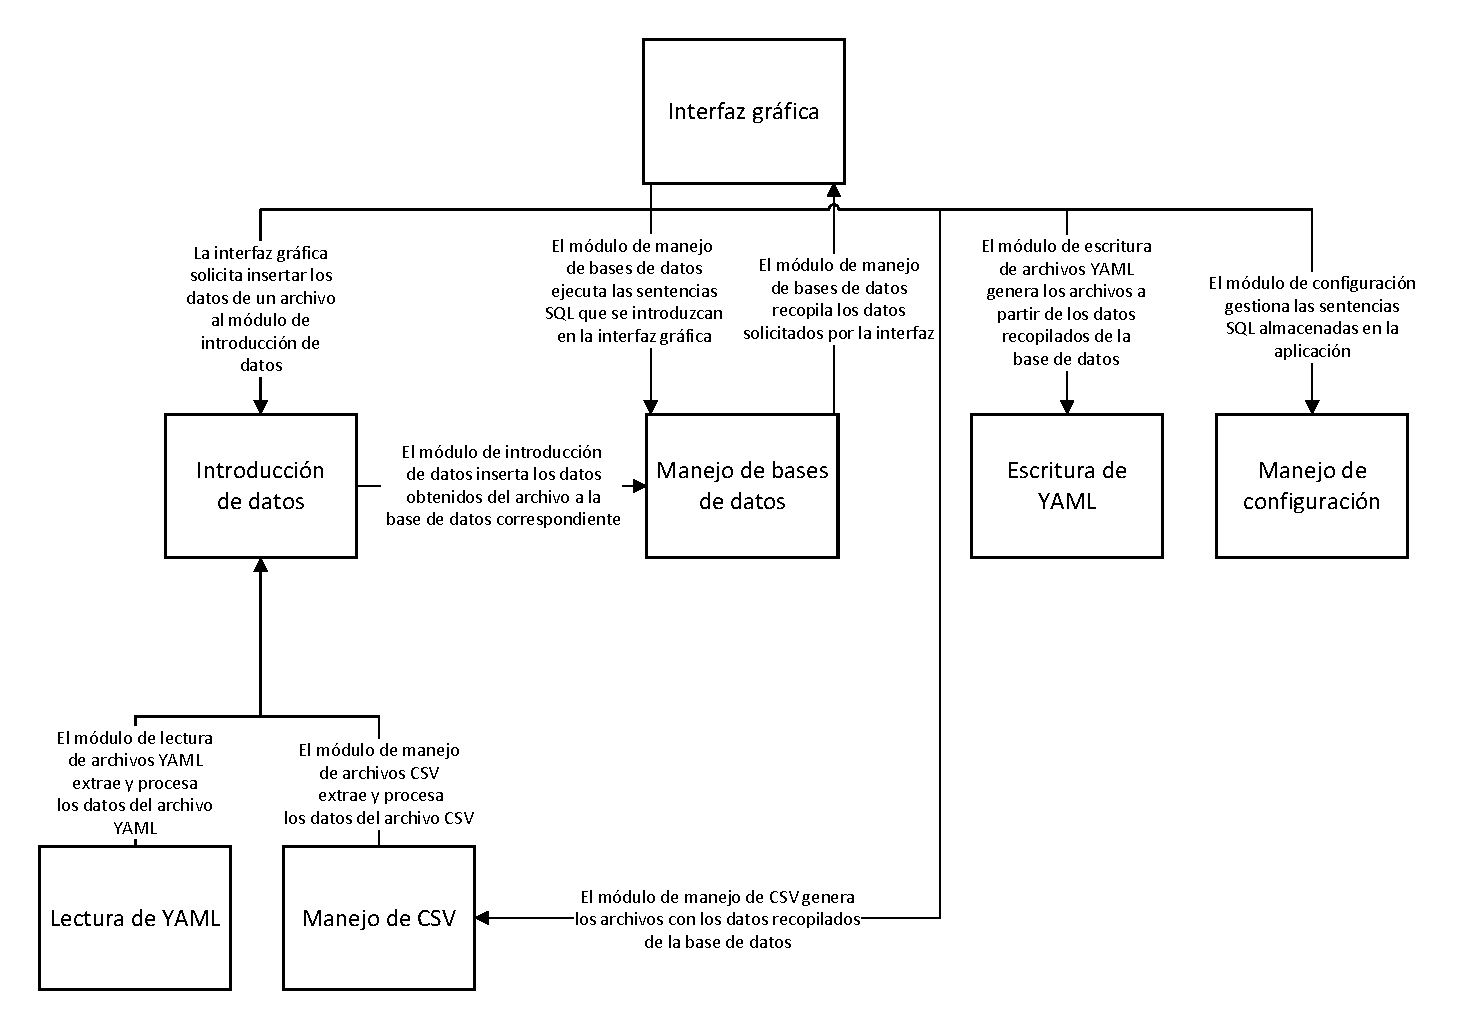
\includegraphics[width=1\textwidth]{fig/Diagramas/Modulos de programa.pdf}
\caption{Diagrama que muestra las relaciones entre los módulos en los que se ha dividido el programa}
\label{fig:DiagramaModulosPrograma}
\end{figure}

A continuación se detalla la función de cada uno de los módulos, así como el archivo Python que contiene el código asociado al mismo:
\begin{itemize}
    \item \texttt{Interfaz Gráfica (UI.py)}: Es el programa principal que maneja la interfaz y todos los demás procesos que hacen funcionar la aplicación.
    \item \texttt{Lectura de Yaml (yamlParser.py)}: Módulo encargado de la lectura  de los datos contenidos en los archivos Yaml de la configuración de la oferta y la demanda.
    \item \texttt{Escritura de Yaml (yamlWriter.py)}: Módulo encargado de la escritura de los archivos Yaml exportados desde las bases de datos.
    \item \texttt{Manejo de bases de datos (SQLHandler.py)}: Módulo encargado de toda la comunicación con las bases de datos.
    \item \texttt{Introducción de datos (dataLoger.py)}: Módulo encargado de introducir los datos empleando los módulos \texttt{yamlParser.py}, \texttt{csvHandler.py} y \texttt{SQLHandler.py} en la base de datos correspondiente. 
    \item \texttt{Manejo de CSV (csvHandler.py)}: Módulo encargado de leer y formatear los datos obtenidos de la simulación para introducirlos en la base de datos de los resultados.
    \item \texttt{Configuración (configManager.py)}: Módulo encargado de gestionar la configuración de la aplicación.
\end{itemize}

Todos los módulos mencionados y de los que se va a hablar en las siguientes secciones, se encuentran en la carpeta \href{https://github.com/Sergioba99/TFG-Gestor_De_Bases_de_Datos/tree/master/Modules}{Modules}\footnote{\url{https://github.com/Sergioba99/TFG-Gestor\_De\_Bases\_de\_Datos/tree/master/Modules}} dentro del repositorio de GitHub. A continuación, se detalla el funcionamiento de cada uno de ellos.

\subsubsection{Módulo de lectura de Yaml}

El módulo \texttt{yamlParser.py} está diseñado para extraer los datos de los archivos Yaml, para después introducirlos en la base de datos empleando el módulo \texttt{dataLoger.py}, que a su vez emplea el módulo \texttt{SQLHandler.py} para introducir la información extraída a la base de datos.

Los archivos \acrshort{Yaml} de entrada de datos de la oferta de los que han de extraerse la información siguen una estructura como la que se ha explicado en la Sección~\ref{sec:archivosEntradaSalida}. La plantilla estructural que siguen estos archivos puede verse en el anexo~\ref{apx:estructuraYamlOferta}. A continuación, se muestra un archivo de ejemplo (Listado~\ref{src:ejemploYamlConfigOferta}) que sigue la estructura de los archivos \acrshort{Yaml} de la configuración de la oferta (Anexo~\ref{apx:estructuraYamlOferta}).

\begin{lstlisting}[language=YAML,
                   frame=none,
                   numbers=none,
                   basicstyle=\ttfamily\normalsize,
                   caption={Ejemplo de archivo Yaml de entrada de datos de la oferta},
                   label=src:ejemploYamlConfigOferta,
                   inputencoding=utf8]                   
stations:
- id: '00001'
  name: Ejemplo1
  city: Ciudad1
  short_name: EJ1
  coordinates:
    latitude: 1.00000000
    longitude: 1.00000000

- id: '00002'
  name: Ejemplo2
  city: Ciudad2
  short_name: EJ2
  coordinates:
    latitude: 2.00000000
    longitude: 2.00000000

seat:
- id: '0'
  name: asientoEjemplo
  hard_type: 0
  soft_type: 0
  
corridor:
- id: '0'
  name: corredorEjemplo
  stations:
  - org: '00001'
    des:
    - org: '00002'
      des: []

line:
- id: '00001'
  name: Line 00001
  corridor: '0'
  stops:
    - station: '00001'
      arrival_time: 0
      departure_time: 0
    - station: '00002'
      arrival_time: 55
      departure_time: 56

rollingStock:
- id: '0'
  name: TrenEjemplo
  seats:
  - hard_type: 0
    quantity: 2

trainServiceProvider:
- id: '0'
  name: ProveedorEjemplo
  rolling_stock:
  - '0'
  
timeSlot:
- id: '00001'
  start: '00:00:00'
  end: '00:10:00'

service:
- id: 00001_06-09-2023-00.00
  date: '2023-09-06'
  line: '00001'
  train_service_provider: '0'
  time_slot: '00001'
  rolling_stock: '0'
  origin_destination_tuples:
  - origin: '00001'
    destination: '00002'
    seats:
    - seat: '0'
      price: 0
  capacity_constraints: null
\end{lstlisting}

En el archivo de ejemplo, se puede ver que hay 8 claves raíz, que son:
\begin{itemize}
    \item \texttt{stations}: En esta clave raíz se encuentran los datos de todas las estaciones que se vayan a emplear en las simulaciones de los servicios descritos en este archivo.
    \item \texttt{seat}: Aquí se almacenan los datos de los diferentes tipos de asiento, como su nombre, el tipo de asiento físico y los beneficios asociados a este.
    \item \texttt{corridor}: Información sobre los corredores ferroviarios que serán utilizados en la simulación.
    \item \texttt{line}: Datos sobre las diferentes lineas que se empleen en las simulaciones.
    \item \texttt{rollingStock}: Caracteristicas sobre los diferentes trenes que van a circular por los corredores para satisfacer los servicios definidos para la simulación.
    \item \texttt{trainServiceProvider}: Información sobre los diferentes proveedores de servicios ferroviarios, que van a prestar servicios en la simulación.
    \item \texttt{timeSlot}: Aquí se encuentran los diferentes intervalos de tiempo en los que los trenes se encuentran estacionados en el anden.
    \item \texttt{service}: Información sobre los diferentes servicios que van a ofrecerse a lo largo del día.
\end{itemize}

Para obtener los datos de este archivo, como se ha comentado previamente, se ha empleado la librería PyYaml. Esta librería transforma los datos contenidos en el archivo \acrshort{Yaml} a tipos de variables existentes en Python (diccionarios, listas, etc.). El siguiente diccionario es un ejemplo de la salida que tendría el archivo \acrshort{Yaml} de ejemplo anterior (Listado~\ref{src:ejemploYamlConfigOferta}) para la clave de \texttt{stations}:

\begin{lstlisting}[language=Python,
                   style=python,
                   frame=none,
                   numbers=none,
                   basicstyle=\ttfamily\normalsize,
                   caption={Diccionario de salida de \texttt{stations}},
                   label=src:diccOutputStations,
                   inputencoding=utf8]                   
{
    "stations": [
        {
            "id": "00001",
            "name": "Ejemplo1",
            "city": "Ciudad1",
            "short_name": "EJ1",
            "coordinates": {
                "latitude": 1.00000000,
                "longitude": 1.00000000
            }
        },
        {
            "id": "00002",
            "name": "Ejemplo2",
            "city": "Ciudad2",
            "short_name": "EJ2",
            "coordinates": {
                "latitude": 2.00000000,
                "longitude": 2.00000000
            }
        }
    ]
}
\end{lstlisting}

%Una vez obtenido el diccionario que contiene todos los datos del archivo \acrshort{Yaml}, bastará con ir accediendo a los diferentes datos mediante las claves e índices que se relacionan con los datos. Por ejemplo, si se quisiera extraer el nombre de la primera estación, se accedería de la siguiente forma: \texttt{datosDeOferta["stations"][0].get("name")}. Esto nos devolvería el valor del nombre de la primera estación, en este caso, "Ejemplo1".

Para poder acceder a los datos de los diferentes archivos que el usuario quiera introducir a la base de datos, primero se ha de abrir el archivo específico mediante el uso de la función \texttt{loadSupplyFile} (Listado~\ref{src:functionLoadSupplyFile}), en caso de que sea un archivo de configuración de oferta, y \texttt{loadDemandFile}, en caso de que el archivo de configuración sea para la demanda.
Estas dos funciones se encuentran dentro de la clase \texttt{Parser} en el módulo \texttt{yamlParser.py}.

 El comportamiento de la función \texttt{loadSupplyFile} (Listado~\ref{src:functionLoadSupplyFile}) se muestra en el diagrama de flujo de la Figura~\ref{fig:DiagramaFlujoLoadSupplyFile}. Su proceso es el siguiente:
\begin{enumerate}
    \item \textit{Selección de archivo}: Abre una ventana de selección de archivo usando la función de Tkinter \texttt{filedialog.askopenfilename} que devuelve la ruta completa al archivo seleccionado por el usuario.
    \item \textit{Comprobación ruta}: Después, se comprueba que esta ruta no esté vacía para, posteriormente, asignarla como valor de la variable de la clase \texttt{Parser}: \texttt{self.supplyFilePath}. Si la ruta está vacía o contiene el valor \texttt{None}, la función interrumpe su ejecución y lanza el error personalizado \texttt{SupplyFileNotFound} que hace que la función devuelva un valor de -2.
    \item \textit{Comprobación errores}: En caso de que ocurra otro error distinto al mencionado durante la ejecución, se devuelve el valor -1.
    \item \textit{Carga de archivo}: En caso de que ningún error suceda, se extrae el nombre del archivo de la ruta y se almacena en la variable \texttt{self.supplyFileName} y se ejecuta la función \texttt{self.getRawDataFromSupply} que carga los datos de todo el archivo \acrshort{Yaml} a la variable \texttt{self.supplyData}. 
\end{enumerate}

\begin{figure}[H]
\centering
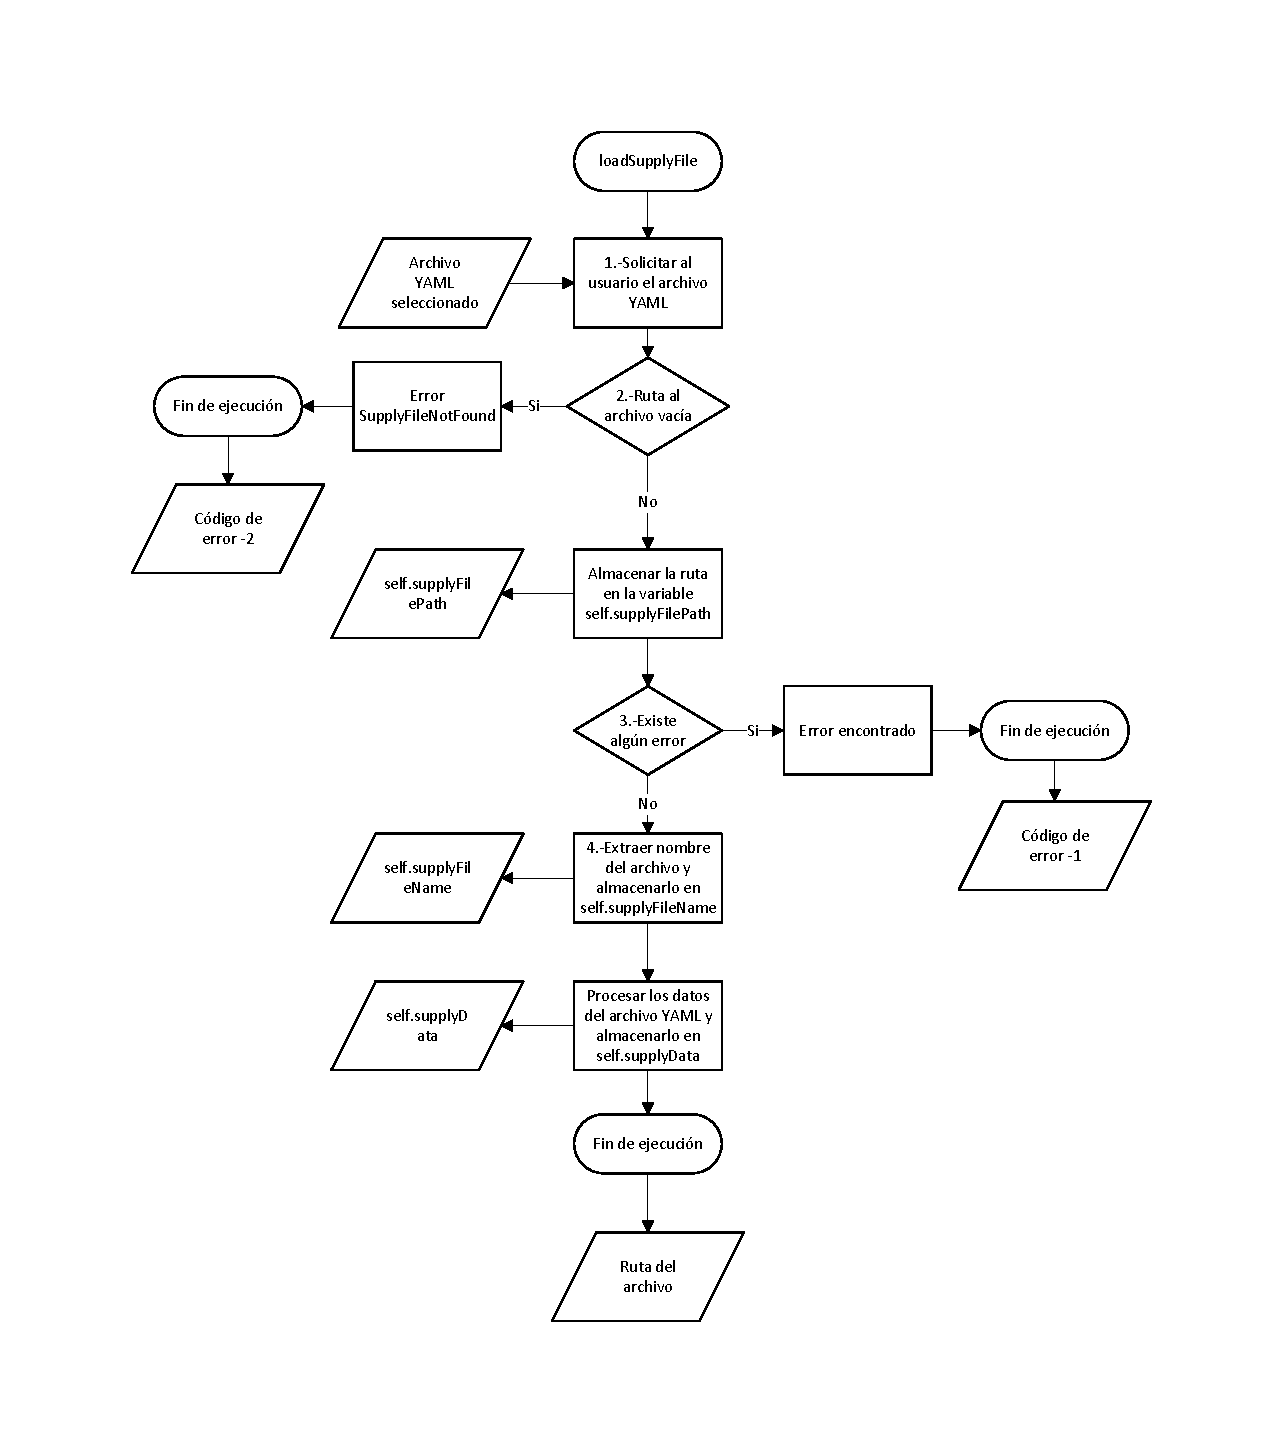
\includegraphics[width=.92\textwidth]{fig/Diagramas de flujo/loadSupplyFile.pdf}
\caption{Diagrama de flujo que muestra el proceso de lectura de un archivo \acrshort{Yaml} mediante \texttt{loadSupplyFile}.}
\label{fig:DiagramaFlujoLoadSupplyFile}
\end{figure}

\begin{lstlisting}[language=Python,
                   style=python,
                   frame=none,
                   numbers=none,
                   basicstyle=\ttfamily\normalsize,
                   caption={Función \texttt{loadSupplyFile}},
                   label=src:functionLoadSupplyFile,
                   inputencoding=utf8]                   
def loadSupplyFile(self):
    try:
        f = filedialog.askopenfilename(
            title="Seleccionar archivo de oferta", initialdir=self.defaultInputDataFolder,
            filetypes=[("Archivos YAML", "*.yml"), ("Todos los archivos", "*.*")], defaultextension=".yml")
        if f != "":
            self.supplyFilePath = f.replace("/", "/")
        else:
            self.supplyFilePath = ""
            self.supplyFileName = ""
        if self.supplyFilePath is None or self.supplyFilePath == '':
            #print("Archivo de oferta no seleccionado")
            raise SupplyFileNotFound

        self.supplyFileName = self.supplyFilePath.split("/")[-1].split(".")[0]
        self.getRawDataFromSupply()
        return f

    except SupplyFileNotFound:
        return -2

    except Exception as e:
        print(e)
        return -1
\end{lstlisting}

%Una vez obtenidos todos los datos almacenados del archivo de configuración de la oferta, se extraen los datos de las diferentes claves raíz. Siguiendo con el ejemplo de la clave raíz \texttt{stations}, para extraer los datos de las estaciones se emplea la función \texttt{getStationsData} (Listado~\ref{src:functionGetStationsData}). Esta función genera y devuelve una lista de listas con todos los datos de la clave raíz \texttt{stations}.

Una vez obtenidos todos los datos almacenados del archivo de configuración de la oferta, se extraen los datos de las diferentes claves raíz. Continuando con el ejemplo de la clave raíz \texttt{stations}, para la extracción de los datos de las diferentes estaciones que aparecen en el archivo de entrada de datos de la oferta, se emplea la función \texttt{getStationsData} (Listado~\ref{src:functionGetStationsData}), cuyo comportamiento se refleja en el diagrama de flujo de la Figura~\ref{fig:DiagramaFlujoGetStationsData}. El proceso que sigue la función \texttt{getStationsData} es el siguiente:
\begin{enumerate}
    \item \textit{Obtención de datos:} Se obtienen los datos de todas las estaciones del archivo de entrada de datos de la oferta que se ha cargado previamente. Estos datos están almacenados como una lista de diccionarios.
    \item \textit{Procesado de datos:} Se construye una lista de listas, a partir de los datos de las estaciones, donde cada sublista contiene el identificador de la estación, el nombre, la ciudad en la que está ubicada, el nombre corto que tenga asignado y, por último, un diccionario con las coordenadas donde se encuentra emplazada la estación, en ese orden. 
    \item \textit{Datos de retorno:} Por último, se devuelve la lista de listas construida.
\end{enumerate}

\begin{figure}[htbp]
\centering
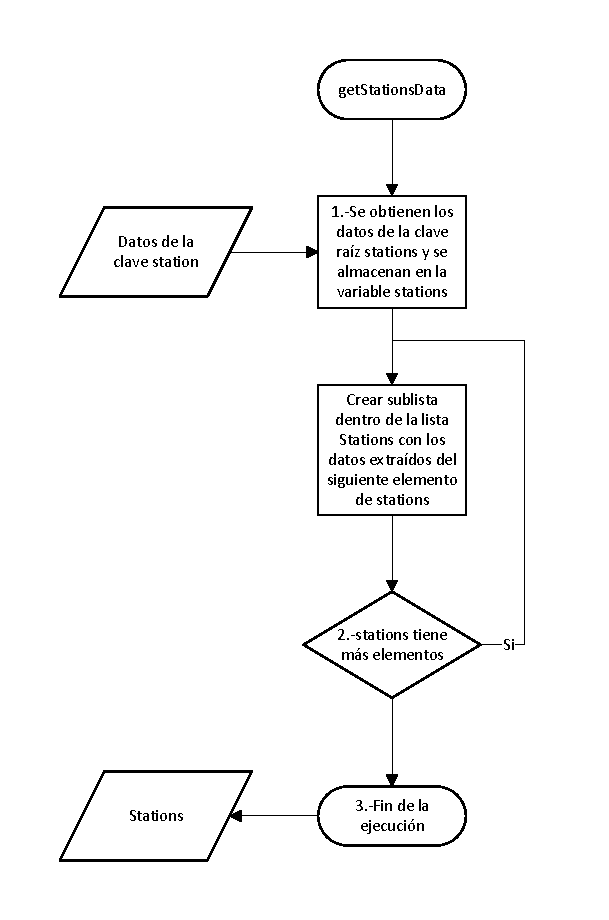
\includegraphics[width=.5\textwidth]{fig/Diagramas de flujo/getStationsData.pdf}
\caption{Diagrama de flujo del proceso de extracción y procesado de los datos de la clave raíz \texttt{stations} con \texttt{getStationsData}.}
\label{fig:DiagramaFlujoGetStationsData}
\end{figure}

\begin{lstlisting}[language=Python,
                   style=python,
                   frame=none,
                   numbers=none,
                   basicstyle=\ttfamily\normalsize,
                   caption={Función \texttt{getStationsData}},
                   label=src:functionGetStationsData,
                   inputencoding=utf8]                   
def getStationsData(self):
    """
    Funcion que devuelve todos los campos de stations en la posicion index ordenados en una lista como en el archivo Yaml.\n
    Salida: [<id>,<name>,<city>,<shortName>,{"latitude":>lat>,"longitude":<lon>}]
    :return: Devuelve el value de stations en la posicion index.
    """
    Stations = []
    try:
        if self.supplyData is None: raise EmptySupplyData
        stations = self.getStations()
        Stations = [[
                    data.get("id"),
                    data.get("name"),
                    data.get("city"),
                    data.get("short_name"),
                    json.dumps(data.get("coordinates"))]
                    for data in stations
                    ]
        return Stations
    except IndexError:
        print("Se ha sobrepasado el índice máximo")
        return "indexError"
    except Exception as e:
        print(e)
        return -1
\end{lstlisting}

Para el resto de claves raíz, las diferentes funciones que extraen sus datos funcionan de manera similar. La diferencia entre las funciones que extraen datos de las claves raíz son las claves que se emplean para recuperar los datos de los diccionarios donde se encuentra la información, salvo unas excepciones que necesitan emplear funciones auxiliares para el acondicionamiento de los datos.

Como se ha mencionado, existen funciones que deben emplear una función auxiliar para adecuar los datos a la estructura de la base de datos o darles un formato que, mediante un procesado simple, permita la inserción de los datos en la tabla correspondiente dentro de la base de datos. Estas funciones son: \texttt{getCorridorData}, \texttt{getLineData}, \texttt{getRollingStockData} y \texttt{getServiceData}. 

Para el caso de la función \texttt{getCorridorData}, que extrae los datos de los corredores ferroviarios bajo la clave raíz \texttt{corridor}, los datos que tienen una estructura que no permite insertarlos directamente a la base de datos son las diferentes estaciones que componen el corredor. Como se puede apreciar en el ejemplo del archivo de configuración de la oferta (Listado~\ref{src:ejemploYamlConfigOferta}), su estructura se compone de un diccionario donde la clave \texttt{org} contiene el identificador de la estación de origen, mientras que la clave \texttt{des} contiene otro diccionario con la misma estructura; es decir una nueva clave \texttt{org}, con el identificador de la estación de origen y una clave \texttt{des}. La clave \texttt{des} puede contener sucesivamente otro diccionario con la misma estructura, hasta que la estación referenciada en \texttt{org} sea la última del corredor, en cuyo caso aparece una lista vacía; es decir, \texttt{[]}.

%La función auxiliar encargada de dar un formato válido a las estaciones que componen el corredor es \texttt{extractStationsFromCorridor} (Listado~\ref{src:functionExtractStationsFromCorridor}). Esta función extrae todas las estaciones que componen el corredor de los datos contenidos en la clave \texttt{stations} dentro de la clave raíz \texttt{corridor} y las agrupa en una lista, en caso de que el corredor no tuviera nada más que un ramal, donde el primer elemento es la estación desde la que parte el corredor y el último elemento sería la estación donde finaliza el corredor o en una lista de listas, en caso de que este corredor tenga ramificaciones, donde cada lista tendrá como primer elemento la primera estación del ramal y como elemento final la última estación del ramal. 

La función auxiliar encargada de extraer los ramales del corredor y darles un formato válido para su posterior inserción a la base de datos es \texttt{extractStationsFromCorridor} (Listado~\ref{src:functionExtractStationsFromCorridor}). Esta función genera una lista de listas donde cada sublista es un ramal del corredor. Estas sublistas contienen los identificadores de las estaciones de los ramales ordenados de manera que el primer elemento de cada una de las sublistas sea la estación donde comienza el ramal y el último elemento corresponde con la estación donde termina. El comportamiento de esta función aparece reflejado en el diagrama de flujo de la Figura~\ref{fig:diagramaFlujoExtractStationsFromCorridor}. El proceso de funcionamiento es:
    \begin{enumerate}
        \item \textit{Comprobar variable \texttt{stations}:} Se comprueba que la variable \texttt{stations} que se pasa como parámetro no tenga el valor \texttt{None}. Si esto ocurre, se le asigna una lista vacía a esta variable, y en caso contrario, se mantiene igual.
        
        \item \textit{Copia de datos:} Se copian los datos de la variable pasada como parámetro \texttt{stationsData} a otra variable denominada \texttt{data}.
        
        \item \textit{Comprobar tipo de \texttt{data}:} Se comprueba si la variable data es una lista o un diccionario. Dependiendo del tipo, se distinguen tres comportamientos:
        
            \begin{enumerate}
                \item \textit{\texttt{data} es una lista:} Si la variable \texttt{data} es una lista, se itera por los diccionario dentro de la lista de tal manera que, se agrega el valor asociado a la clave \texttt{org} a la lista \texttt{newStations}. Se genera una lista nueva denominada \texttt{l2} y se le da el valor asociado a la clave \texttt{des}.
                    \begin{itemize}
                        \item Si \texttt{l2} esta vacía, significa que se ha llegado al final de un ramal, por lo que la lista \texttt{newStations} se agrega a la lista de listas \texttt{allStations}. Tras esto, el programa finaliza y se devuelve el valor de \texttt{allStations} que contiene todos los ramales que existen en el corredor.
                        
                        \item  En caso contrario, se comprueba el tipo de \texttt{l2}, si no es una lista o un diccionario, se agrega la lista \texttt{newStations} a \texttt{allStations}. Después, el programa finaliza y se devuelve el valor de \texttt{allStations} que contiene todos los ramales que existen en el corredor.
                        
                        \item Si por el contrario, \texttt{l2} es un diccionario o una lista, se llama a la función \texttt{extractStationsFromCorridor} pasando como parámetros la variable \texttt{l2}, como el parámetro \texttt{stationsData}, y \texttt{newStations}, como el parámetro \texttt{stations} y el valor que se devuelva de la ejecución se añade a \texttt{allStations}.
                    \end{itemize}
                Este proceso se repite para cada uno de los diccionarios dentro de la lista dentro de \texttt{data}.
                
                \item \textit{\texttt{data} es un diccionario:} Si la variable \texttt{data} es un diccionario, se extrae el valor asociado a la clave \texttt{org} y se añade a \texttt{newStations}. Después, se agrega a \texttt{l2} el valor de la clave \texttt{des}. 
                    \begin{itemize}
                        \item Si \texttt{l2} esta vacía, se agrega el valor de \texttt{newStations} a \texttt{allStations}, se devuelve el valor de \texttt{allStations} y se finaliza la ejecución de la función. 
                        
                        \item Si por el contrario, \texttt{l2}, no esta vacía y se trata de una lista o un diccionario, se llama a la función \texttt{extractStationsFromCorridor} pasando como parámetros la variable \texttt{l2}, como el parámetro \texttt{stationsData}, y \texttt{newStations}, como el parámetro \texttt{stations} y el valor que se retorne de la ejecución se añade a \texttt{allStations}.
                        
                        \item  Si \texttt{l2} no es una lista ni un diccionario, se añade el valor de \texttt{newStations} a \texttt{allStations}, se devuelve \texttt{allStations} y se finaliza la ejecución.
                    \end{itemize}
                    
                \item \textit{\texttt{data} no es ni lista ni diccionario:} Si \texttt{data} no es ni una lista ni un diccionario, se agrega el valor de \texttt{newStations} a \texttt{allStations}, se devuelve el valor de \texttt{allStations} y se finaliza la ejecución de la función.
            \end{enumerate}
    \end{enumerate}

\begin{figure}[hbpt]
\centering
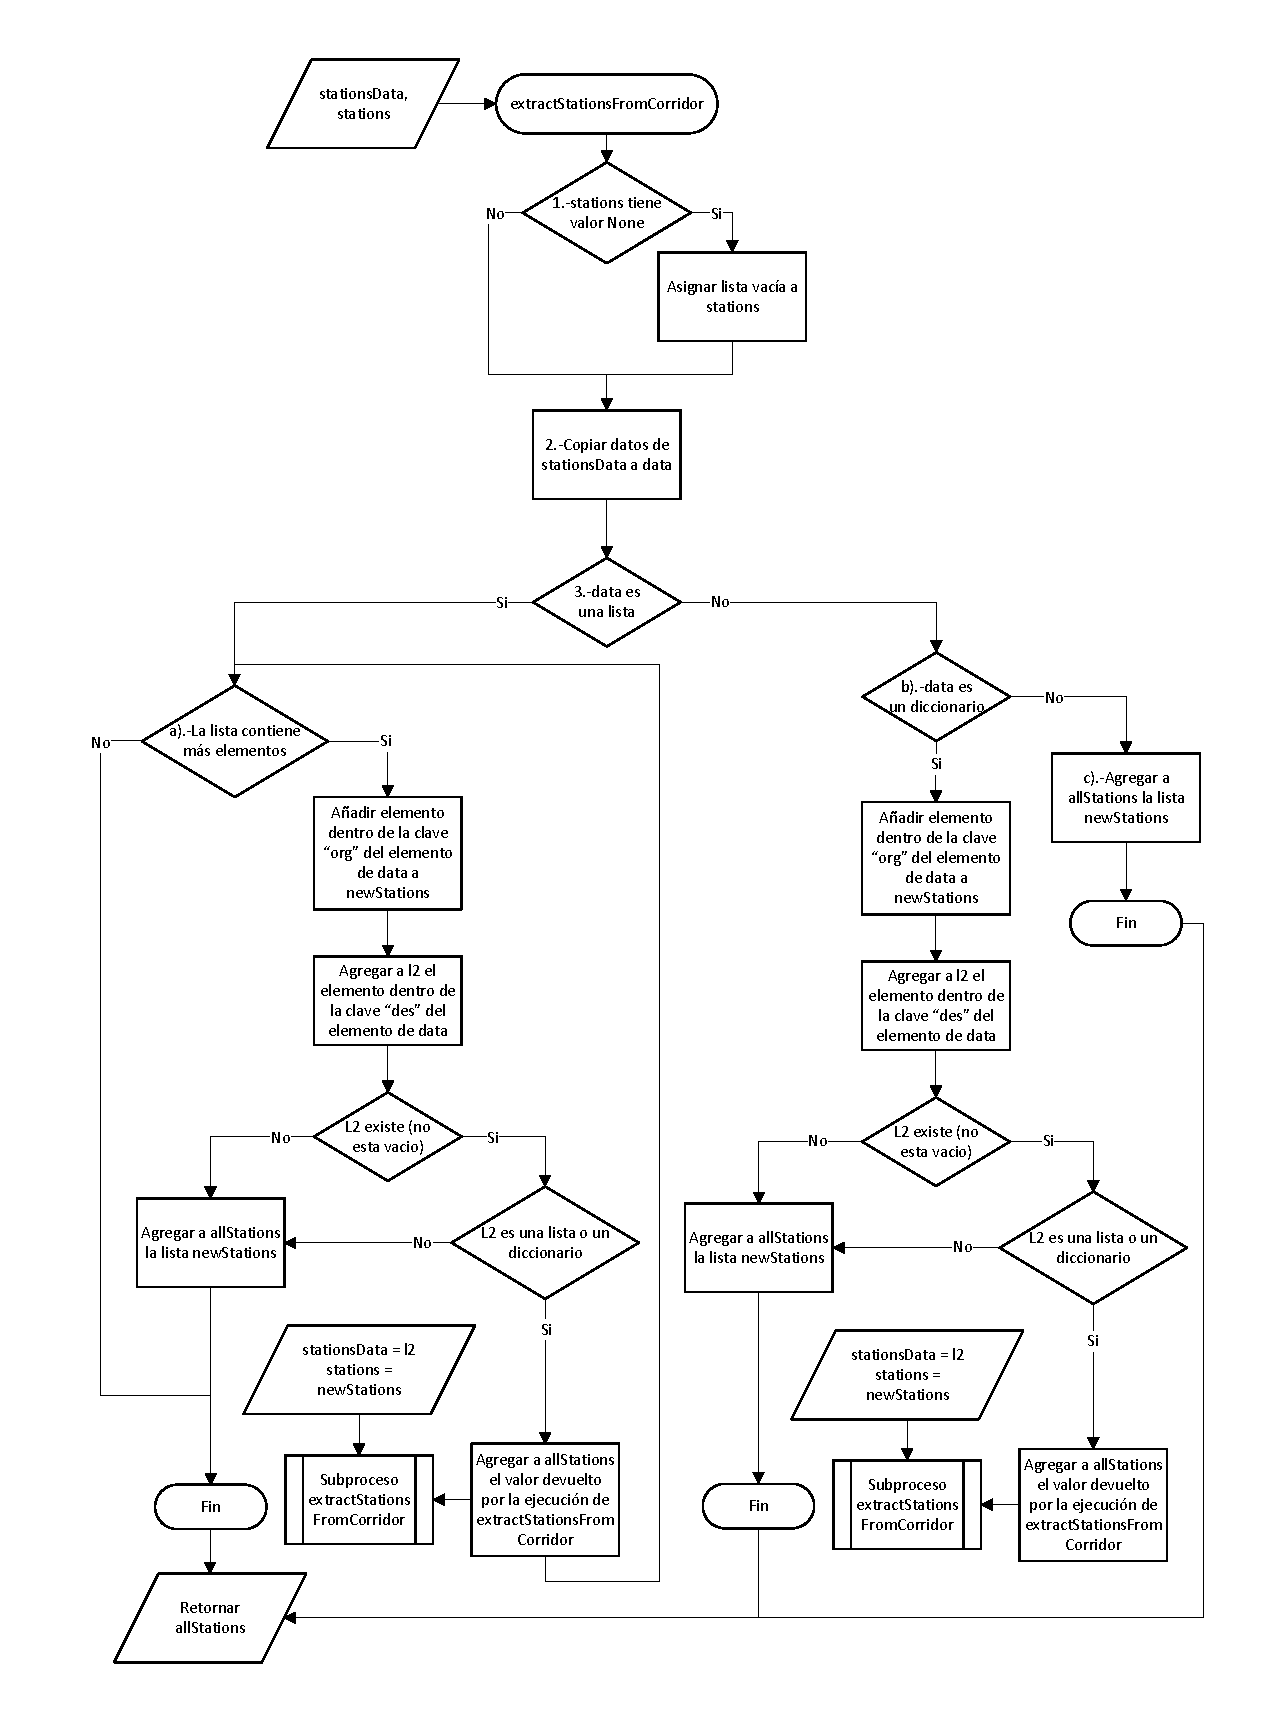
\includegraphics[width=1\textwidth]{fig/Diagramas de flujo/extractStationsFromCorridor.pdf}
\caption{Diagrama de flujo de la función \texttt{extractStationsFromCorridor} }
\label{fig:diagramaFlujoExtractStationsFromCorridor}
\end{figure}

\begin{lstlisting}[language=Python,
                   style=python,
                   frame=none,
                   numbers=none,
                   basicstyle=\ttfamily\normalsize,
                   caption={Función \texttt{extractStationsFromCorridor}},
                   label=src:functionExtractStationsFromCorridor,
                   inputencoding=utf8]                   
        def extractStationsFromCorridor(self, stationsData: list, stations=None):
        """
        Extrae los ramales del corredor. Esta función devuelve una lista
        ordenada con todos los ramales. Cada ramal será una lista ordenada
        siendo el primer elemento la estación de inicio del ramal y el último
        elemento será la última estación del ramal.
        :param stationsData: Lista en las que están contenidos los IDs de
        todas las estaciones por las que va a pasar el
        corredor
        :param stations: Ruta actual acumulada (se utiliza internamente al
        llamar recursivamente).
        :return: Devuelve una lista de listas con todos los ramales del 
        corredor.
        """
        if stations is None:
            stations = []

        # Se hace una copia de stationsData para evitar modificar el original
        data = deepcopy(stationsData)
        allStations = []

        if isinstance(data, list):
            # Se recorre cada elemento de la lista (cada elemento representa
            # un inicio o ramal)
            for item in data:
                newStations = stations.copy()
                newStations.append(item.get("org"))
                l2 = item.get("des")
                if l2:
                    # Si existen destinos, se llama recursivamente (ya sea
                    # que l2 sea lista o diccionario)
                    if isinstance(l2, (list, dict)):
                        allStations.extend(
                            self.extractStationsFromCorridor(l2, newStations))
                    else:
                        allStations.append(newStations)
                else:
                    # No hay más destinos: se agrega la ruta completa
                    allStations.append(newStations)
        elif isinstance(data, dict):
            # Caso en el que data es un único diccionario
            newStations = stations.copy()
            newStations.append(data.get("org"))
            l2 = data.get("des")
            if l2:
                if isinstance(l2, (list, dict)):
                    allStations.extend(
                        self.extractStationsFromCorridor(l2, newStations))
                else:
                    allStations.append(newStations)
            else:
                allStations.append(newStations)
        else:
            # En caso de que data no tenga el formato esperado, se devuelve la
            # ruta actual
            allStations.append(stations)

        return allStations
\end{lstlisting}

Otra de las funciones auxiliares que dan un formato válido a los datos para su inserción a la base de datos, sería la función \texttt{extractStopsFromLine} (Listado~\ref{src:functionExtractStopsFromLine}). Esta función se encarga de extraer la información de las diferentes paradas que se realizan a lo largo de una línea de tren. Esta información está conformada por el identificador de la estación en la que el tren ha de parar, el tiempo de llegada a esa estación y el tiempo de salida de esa estación. La función devuelve una lista de listas, donde cada sublista contiene los datos ya mencionados para que de esta manera, puedan ser introducidos a la tabla \texttt{STOPS} de la base de datos (Figura~\ref{fig:dbSupplySTOPS}).

\begin{lstlisting}[language=Python,
                   style=python,
                   frame=none,
                   numbers=none,
                   basicstyle=\ttfamily\normalsize,
                   caption={Función \texttt{extractStopsFromLine}},
                   label=src:functionExtractStopsFromLine,
                   inputencoding=utf8]                   

def extractStopsFromLine(stopsData: list):
    """
    Esta funcion extrae todas las paradas con sus tiempos de llegada y salida de una linea.
    Devuelve una lista de listas donde cada lista se compone de la parada, tiempo de llegada y tiepo de salida,
    por lo que respeta el orden del archivo Yaml.
    :param stopsData: Lista de diccionarios con los datos de todas las paradas en la linea.
    :return: lista de listas con los datos de todas las paradas de la linea.
    """
    stops = []
    data = deepcopy(stopsData)
    while data:
        stops.append([str(data[0].get("station")), data[0].get("arrival_time"), data[0].get("departure_time")])
        data.pop(0)
    return stops
\end{lstlisting}

La función auxiliar \texttt{extractSeatsFromRollingStock} (Listado~\ref{src:functionExtractSeatsFromRollingStock}) tiene como cometido generar un diccionario donde cada una de las claves del diccionario son los diferentes tipos de asientos físicos del tren. Cada una de estas claves toma como valor el número de asientos del tipo almacenado como clave que posee el tren. Por ejemplo, si un tren tiene 200 asientos del tipo 1 y 50 asientos del tipo 2, el diccionario resultante de ejecutar esta función será: \texttt{\{"1":200,"2":50\}} 

\begin{lstlisting}[language=Python,
                   style=python,
                   frame=none,
                   numbers=none,
                   basicstyle=\ttfamily\normalsize,
                   caption={Función \texttt{extractSeatsFromRollingStock}},
                   label=src:functionExtractSeatsFromRollingStock,
                   inputencoding=utf8]                   

def extractSeatsFromRollingStock(seatsData: list):
    """
    Esta funcion extrae los datos de los asientos de uno de los trenes de rollingStock pasado como parametro.
    Devuelve un diccionario que emplea como key el hard_type y como value para esa key el numero de asientos de
    ese tipo de los que dispone dicho tren.
    :param seatsData: Datos extraidos de seats en rollingStock.
    :return: Devuelve un diccionario con los tipos de asiento y la cantidad de estos.
    """
    seats = {}
    data = deepcopy(seatsData)
    while data:
        seats.update({str(data[0].get("hard_type")): data[0].get("quantity")})
        data.pop(0)
    return seats
\end{lstlisting}

Por último, la función auxiliar \texttt{extractSeatsPriceFromServiceOdt} (Listado~\ref{src:functionExtractSeatsPriceFromServiceOdt}) se encarga de extraer los datos de los orígenes, destinos y precios por asiento que están asociados a la clave \texttt{origin\_destination\_tuples} de un servicio. Estos datos se almacenan en una lista de listas, donde cada lista tiene como primer elemento la estación de origen, seguida de la estación de destino y, por último, un diccionario donde la clave es el tipo de asiento, definido previamente en la clave raíz \texttt{seat}, a la que se le asigna como valor el precio que recibe ese tipo de asiento para ese trayecto entre la estación de origen y la estación de destino.

\begin{lstlisting}[language=Python,
                   style=python,
                   frame=none,
                   numbers=none,
                   basicstyle=\ttfamily\normalsize,
                   caption={Función \texttt{extractSeatsPriceFromServiceOdt}},
                   label=src:functionExtractSeatsPriceFromServiceOdt,
                   inputencoding=utf8]                   

def extractSeatsPriceFromServiceOdt(odtData: list):
    data = deepcopy(odtData)
    outputData = []
    while data:
        price = {}
        seats = data[0].get("seats")
        odt = data[0]
        while seats:
            price.update({str(seats[0].get("seat")): seats[0].get("price")})
            seats.pop(0)
        output = [odt.get("origin"), odt.get("destination"), deepcopy(price)]
        outputData.append(output)
        data.pop(0)
    return outputData
\end{lstlisting}

%Para el archivo de demanda, el procedimiento es similar, primero se carga el archivo de demanda usando la función \texttt{loadDemandFile}, que funciona como la función \texttt{loadSupplyFile} (Listado~\ref{src:functionLoadSupplyFile}), pero en este caso selecciona un archivo de configuración de la demanda. Esta función asigna como valor de la variable \texttt{self.demandFilePath} la ruta hasta el archivo seleccionado, extrae el nombre del archivo y lo almacena en la variable \texttt{self.demandFileName} y, por último, carga los datos empleando la función \texttt{self.getRawDataFromDemand} y los guarda en la variable \texttt{self.demandData}. 

Para cargar el archivo de entrada de datos de la demanda, el procedimiento es similar al empleado por la función \texttt{loadSupplyFile} (Listado~\ref{src:functionLoadSupplyFile}). La función encargada de esta tarea es \texttt{loadDemandFile} y su comportamiento aparece reflejado en el diagrama de flujo de la Figura~\ref{fig:DiagramaFlujoLoadDemandFile}. El procedimiento que sigue la función es el siguiente:
\begin{enumerate}
    \item \textit{Selección de archivo:} Abre una ventana de selección de archivo usando una función de Tkinter denominada \texttt{filedialog.askopenfilename}, que devuelve la ruta completa al archivo seleccionado.
    \item \textit{Comprobación de ruta:} Después, se comprueba que la ruta no este vacía para asignarla como valor de la variable \texttt{self.demandFilePath}. En caso de que la ruta esté vacía o contenga el valor \texttt{None}, la función interrumpe su ejecución normal lanzando el error personalizado \texttt{DemandFileNotFound}, para acto seguido, devolver el valor -2.
    \item \textit{Comprobación de errores:} En caso de que ocurra otro error diferente al mencionado durante la ejecución, se detiene la ejecución normal de la función se devuelve el valor -1.
    \item \textit{Carga de archivo:} Si ningún error sucede, se extrae el nombre del archivo de la ruta y se almacena en la variable \texttt{self.demandFileName} y se ejecuta la función \texttt{getRawDataFromDemand} que carga los datos de todo el archivo \acrshort{Yaml} a la variable \texttt{self.demandData}.
\end{enumerate}


\begin{figure}[htbp]
\centering
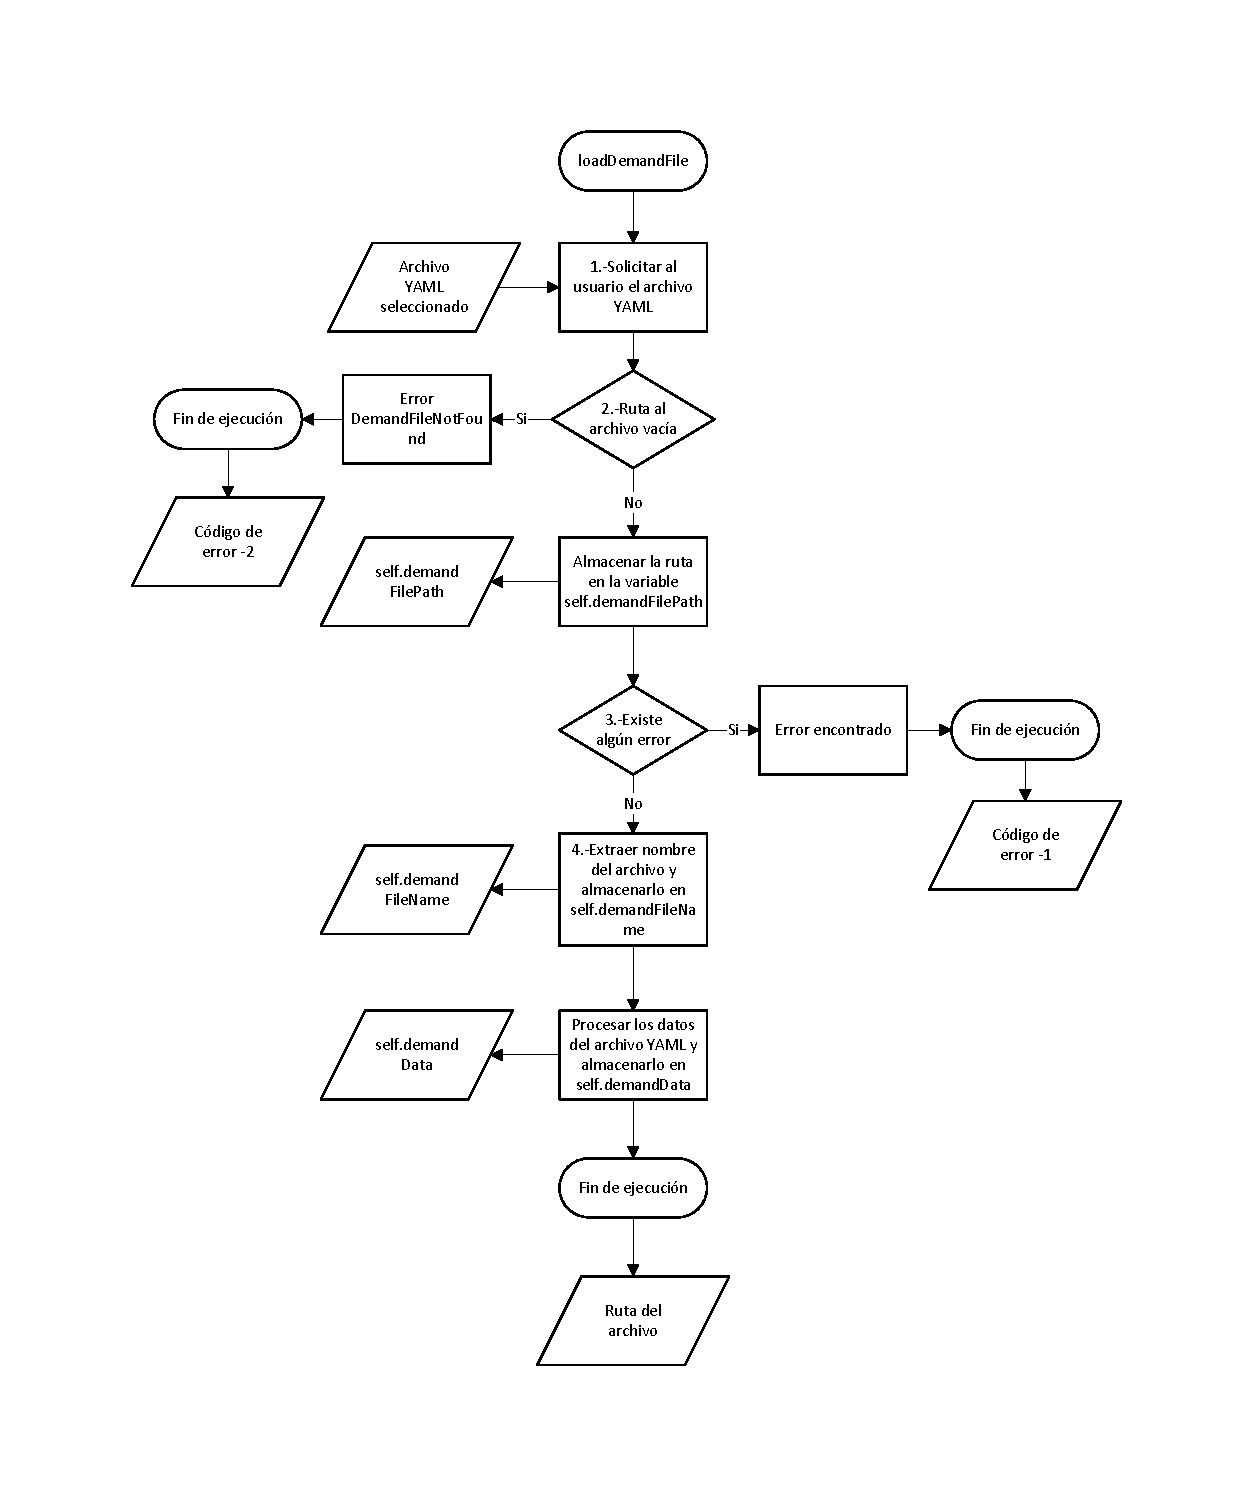
\includegraphics[width=.92\textwidth]{fig/Diagramas de flujo/loadDemandFile.pdf}
\caption{Diagrama de flujo que muestra el proceso de lectura de un archivo \acrshort{Yaml} mediante \texttt{loadDemandFile}.}
\label{fig:DiagramaFlujoLoadDemandFile}
\end{figure}

Al igual que ocurre con los archivos de la oferta, las funciones que extraen los datos del archivo de la demanda son muy similares entre sí, todas obtienen los datos asociados a las claves raíz empleando las claves bajo la clave raíz. Un ejemplo de una función de la demanda es la función \texttt{getMarktetData} (Listado~\ref{src:functionGetMarketData})que devuelve los datos extraídos de la clave raíz \texttt{market} del archivo de configuración de la demanda.

Pero al igual que ocurría con algunas de las funciones destinadas a obtener los datos de los archivos de configuración de la oferta, algunas de las funciones destinadas a obtener los datos del archivo de la demanda necesitan apoyarse en funciones auxiliares para reformar los datos y hacerlos coincidir con lo que espera la base de datos. Estas funciones auxiliares son las siguientes: \texttt{extractMarketsFromDemmandPattern}, \texttt{extractUserPatternDistributionFromMarkets}, \texttt{extractSeatsFromUserPattern}, \texttt{extractTrainServiceProvidersFromUserPattern} y \parbox{\linewidth}{\texttt{reformatVariableSets}}

\begin{lstlisting}[language=Python,
                   style=python,
                   frame=none,
                   numbers=none,
                   basicstyle=\ttfamily\normalsize,
                   caption={Función \texttt{getMarktetData}},
                   label=src:functionGetMarketData,
                   inputencoding=utf8]                   

def getMarketData(self):
    """
    Funcion que devuelve todos los campos de market en la posicion index ordenados en una lista como en el archivo Yaml.\n
    Salida: [<id>,<departure_station>,<[<departure_station_coords>]>,
    <arrival_station>,<timeSlot>,<[<arrival_station_coords>]>]
    :return: Devuelve el value de market en la posicion index.
    """
    Market = []
    try:
        if self.demandData is None: raise EmptyDemandData
        market = self.getMarket()
        Market = [
                    [
                        market[index].get("id"),
                        market[index].get(
                            "departure_station"),
                        json.dumps(market[index].get(
                            "departure_station_coords")),
                        market[index].get(
                            "arrival_station"),
                        json.dumps(market[index].get(
                            "arrival_station_coords"))]

                    for index in range(0,len(market))
                ]

        return Market
    except Exception as e:
        print(e)
        return -1
\end{lstlisting}

La función \texttt{extractMarketsFromDemmandPattern} (Listado~\ref{src:functionExtractMarketsFromDemmandPattern}) extrae los mercados potenciales de la clave \texttt{markets} dentro de la clave raíz \texttt{demandPattern} y los introduce en una lista de listas donde cada lista tiene como primer elemento el identificador que recibe el mercado, seguido de la función que va a utilizar el simulador para calcular la demanda potencial, los parámetros de dicha función y la distribución de los patrones que siguen los usuarios. Este último elemento, a su vez, usa la función auxiliar \texttt{extractUserPatternDistributionFromMarkets} (Listado~\ref{src:functionExtractUserPatternDistributionFromMarkets}) para reformular la distribución de los patrones de usuario.

Estos patrones de usuario, tras usar la función \texttt{extractUserPatternDistributionFromMarkets}, se reformulan en una lista de diccionarios, donde la clave de cada diccionario es el identificador del patrón de usuario, mientras que el valor asociado a esta clave es el porcentaje de usuarios de ese patrón en concreto.

\begin{lstlisting}[language=Python,
                   style=python,
                   frame=none,
                   numbers=none,
                   basicstyle=\ttfamily\normalsize,
                   caption={Función \texttt{extractMarketsFromDemmandPattern}},
                   label=src:functionExtractMarketsFromDemmandPattern,
                   inputencoding=utf8]                   
def extractMarketsFromDemmandPattern(self,marketsData):
    markets = []
    data = deepcopy(marketsData)
    while data:
        markets.append([data[0].get("market"),
                        data[0].get("potential_demand"),
                        json.dumps(data[0].get("potential_demand_kwargs")),
                        self.extractUserPatternDistributionFromMarkets(data[0].get("user_pattern_distribution"))])
        data.pop(0)
    return markets
\end{lstlisting}

\begin{lstlisting}[language=Python,
                   style=python,
                   frame=none,
                   numbers=none,
                   basicstyle=\ttfamily\normalsize,
                   caption={Función \texttt{extractUserPatternDistributionFromMarkets}},
                   label=src:functionExtractUserPatternDistributionFromMarkets,
                   inputencoding=utf8]                   
def extractUserPatternDistributionFromMarkets(UpdData):
    percentage = {}
    data = deepcopy(UpdData)
    while data:
        percentage.update({str(data[0].get("id")): data[0].get("percentage")})
        data.pop(0)
    return percentage
\end{lstlisting}

Las funciones auxiliares \texttt{extractSeatsFromUserPattern} y \texttt{extractTrainServiceProvidersFromUserPattern} funcionan de manera similar a la función \texttt{extractUserPatternDistributionFromMarkets}, forman una lista de diccionarios, donde la clave de cada diccionario es el identificador que recibe el asiento, si la función es \texttt{extractSeatsFromUserPattern} o el identificador que recibe el proveedor de servicios ferroviarios, en caso de que la función sea  \texttt{extractTrainServiceProvidersFromUserPattern} y, como valor referenciado por dicha clave, se toma o bien el valor de utilidad del asiento, si la función es \texttt{extractSeatsFromUserPattern} o bien el valor de utilidad del proveedor de servicios ferroviarios si la función es \texttt{extractTrainServiceProvidersFromUserPattern}.

Por último, la función auxiliar \texttt{reformatVariableSets} es la encargada de reformular los campos de \texttt{variables} en una lista de diccionarios donde cada diccionario tiene almacenada una variable. Cada diccionario contiene unos datos en función del tipo de variable. Si la variable es del tipo "fuzzy", este diccionario contiene el nombre, el tipo, en este caso "fuzzy", el dominio de la variable lingüística y, por último, los conjuntos difusos. Si la variable es "categorical", el diccionario contiene el nombre, el tipo, en este caso "categorical" y la lista de etiquetas de la variable.

\begin{lstlisting}[language=Python,
                   style=python,
                   frame=none,
                   numbers=none,
                   basicstyle=\ttfamily\normalsize,
                   caption={Función \texttt{reformatVariableSets}},
                   label=src:functionReformatVariableSets,
                   inputencoding=utf8]                   
def reformatVariableSets(variableData:dict):
    outputData = []
    for varData in variableData:
        if "labels" in varData.keys(): outputData.append(varData)
        else:
            data = deepcopy(varData)
            variables = {"name":data.get("name"),"type":data.get("type"),"support":data.get("support")}
            setsData = data.get("sets")
            sets = {}
            while setsData:
                sets.update({str(setsData[0]):data.get(setsData[0])})
                setsData.pop(0)
            variables.update({"sets":sets})
            outputData.append(variables)
    return outputData
\end{lstlisting}



\subsubsection{Módulo de escritura de Yaml}

El módulo \texttt{yamlWriter.py} está diseñado para reconstruir los archivos \acrshort{Yaml} empleando los datos provenientes de las bases de datos. Estos archivos reconstruidos se guardan en la ubicación que el usuario designe mediante una ventana de selección de carpeta. La ubicación que abre la ventana de selección de carpeta, por defecto, se encuentra ubicada en el directorio de trabajo de la aplicación, normalmente, es la misma carpeta que el ejecutable, dentro de la carpeta "outputData". Esta carpeta se genera la primera vez que se ejecuta el programa o cuando la carpeta no existe dentro del directorio de trabajo.

La función \texttt{saveFile} de la clase \texttt{Writer} del módulo se emplea para generar archivos \acrshort{Yaml} a partir de los datos que se van a insertar en él y del nombre que va a recibir el archivo, ambos pasados como parámetros a la función. El comportamiento de la función puede observarse en el diagrama de flujo de la Figura~\ref{fig:DiagramaFlujoSaveFile}. El proceso seguido por la función es:
\begin{enumerate}
    \item \textit{Seleccionar ubicación de guardado:} Abre una ventana de selección de carpeta empleando la función de Tkinter \texttt{filedialog.askdirectory}, que devuelve la ruta a la carpeta seleccionada.
    \item \textit{Comprobar ruta:} Se comprueba que la ruta no esté vacía. Si la ruta se encuentra vacía, la función detiene su ejecución.
    \item \textit{Generar archivo:} Se genera un archivo en blanco con el nombre que se ha introducido antes como parámetro.
    \item \textit{Insertar datos:} Se insertan los datos pasados como parámetro en el archivo recién creado.
\end{enumerate}

\begin{figure}[htbp]
\centering
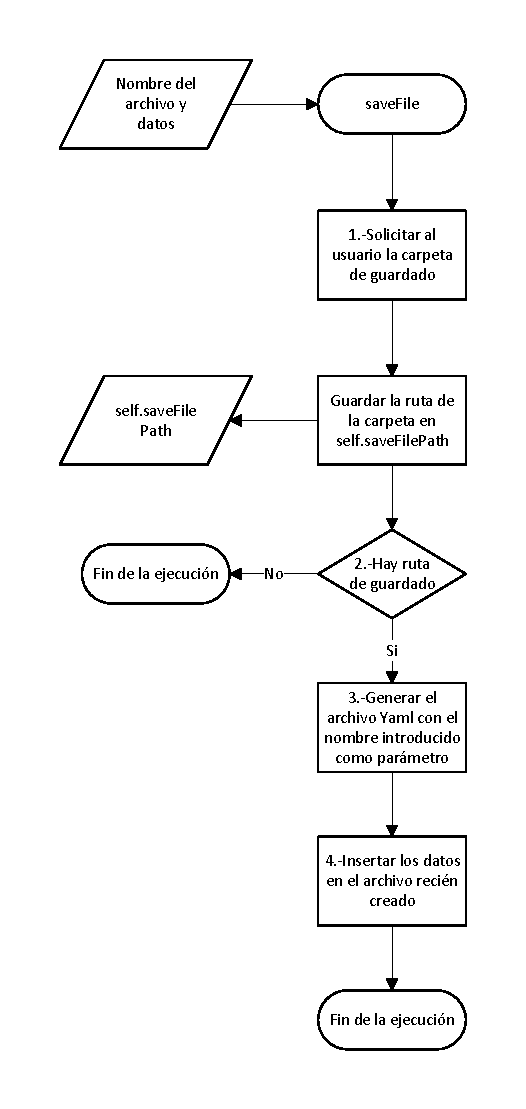
\includegraphics[width=.47\textwidth]{fig/Diagramas de flujo/saveFile.pdf}
\caption{Diagrama de flujo que muestra el proceso de guardado de un archivo \acrshort{Yaml} mediante \texttt{saveFile}.}
\label{fig:DiagramaFlujoSaveFile}
\end{figure}

%Para guardar los archivos se emplea la función \texttt{saveFile} de la clase \texttt{Writer} del módulo. Esta función necesita que se le pasen como parámetros el nombre que va a recibir el archivo y los datos que van a ser escritos en él. La función pide al usuario que seleccione la carpeta donde ha de guardar el archivo que va a ser generado. Tras seleccionar la carpeta, la ruta a esta se almacena en la variable \texttt{self.saveFilePath}. Después, se comprueba que dicha ruta no esté vacía, debido a que el usuario haya cancelado la acción o haya cerrado la ventana de selección de la carpeta. Si no hay ningún problema, se procede a crear el archivo \acrshort{Yaml}, con el nombre que se ha pasado como argumento, en la ruta especificada y, una vez creado, se introducen los datos que se han pasado como parámetro al archivo recién creado. Este comportamiento se puede ver en el diagrama de la Figura~\ref{fig:DiagramaFlujoSaveFile}.

\subsubsection{Módulo de manejo de CSV}

\texttt{CsvHandler.py} es el módulo encargado de leer los archivos \acrshort{CSV} que arroja el simulador con los resultados de las simulaciones realizadas y generar los archivos \acrshort{CSV} con la información de la base de datos. Este módulo se compone de dos clases: \texttt{csvReader} y \texttt{csvWriter}

La clase \texttt{csvReader} contiene las funciones necesarias para obtener los datos de los resultados de los archivos \acrshort{CSV}. Para obtener dichos datos, se usa la función \texttt{loadCsvFile} (Listado~\ref{src:functionLoadCsvFile}). El comportamiento de esta función se encuentra representado en el diagrama de flujo de la Figura~\ref{fig:DiagramaFlujoLoadCsvFile}. Su proceso es el siguiente:
\begin{enumerate}
    \item \textit{Selección del archivo:} Se utiliza una ventana de selección de archivo para obtener la ruta del archivo seleccionado por el usuario. Esta ventana se genera con la función \texttt{filedialog.askopenfilename} de Tkinter.
    \item \textit{Comprobación de ruta:} Se comprueba que la ruta obtenida no este vacía para asignarla como valor de la variable \texttt{self.csvFilePath}. Si la ruta está vacía, o posee el valor \texttt{None}, la función detiene su ejecución, lanza el error personalizado \texttt{CsvFileNotFound} y devuelve el valor -2.
    \item \textit{Comprobación de errores:} Si llega a darse un error durante la ejecución diferente al mencionado, se detiene la ejecución de la función y se devuelve el valor -1.
    \item \textit{Carga de archivo:} En caso de que no se haya producido ningún error, se extrae el nombre del archivo de la ruta almacenada y se almacena en la variable \texttt{self.csvFileName}. Después, se ejecuta la función \texttt{getRawDataFromCsv}, que carga los datos a la variable \texttt{self.csvData}.
\end{enumerate}

%Esta función requiere que el usuario seleccione el archivo que quiere introducir en la base de datos. Una vez seleccionado, se comprueba que la ruta al archivo se ha cargado bien. Si dicha ruta existe, se guarda dicha ruta en la variable \texttt{self.csvFilePath} y de esta ruta se extrae el nombre del archivo para almacenarlo en la variable \texttt{self.csvFileName}. Después, se ejecuta la función \texttt{getRawDataFromCsv} para obtener la información del archivo. 

\begin{figure}[H]
\centering
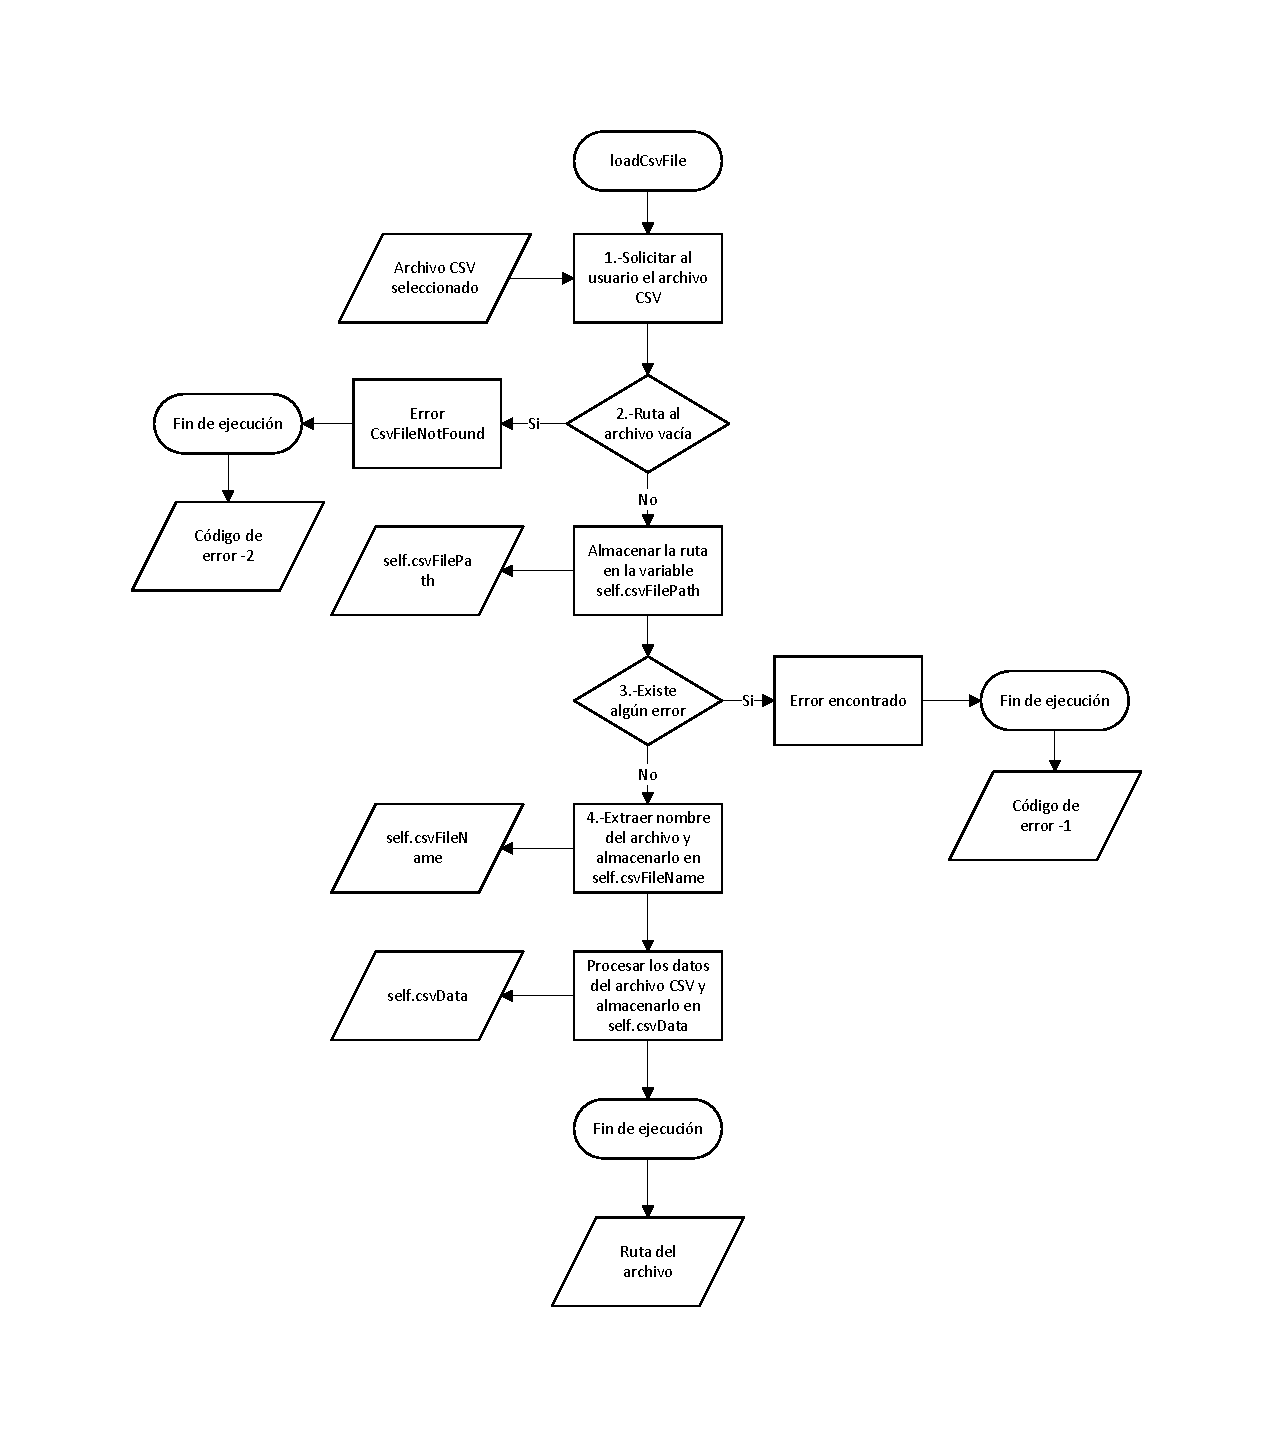
\includegraphics[width=.92\textwidth]{fig/Diagramas de flujo/loadCsvFile.pdf}
\caption{Diagrama de flujo que muestra el proceso de lectura de un archivo \acrshort{CSV} mediante \texttt{loadCsvFile}.}
\label{fig:DiagramaFlujoLoadCsvFile}
\end{figure}

\begin{lstlisting}[language=Python,
                   style=python,
                   frame=none,
                   numbers=none,
                   basicstyle=\ttfamily\normalsize,
                   caption={Función \texttt{loadCsvFile}},
                   label=src:functionLoadCsvFile,
                   inputencoding=utf8]                   
def loadCsvFile(self):
    try:
        f = filedialog.askopenfilename(title="Seleccionar archivo de resultados",
                                       initialdir=self.defaultInputDataFolder,
                                       filetypes=[("Archivos CSV", "*.csv"), ("Todos los archivos", "*.*")],
                                       defaultextension=".csv")

        if f != "":
            self.csvFilePath = f.replace("/", "/")
        if self.csvFilePath is None or self.csvFilePath == '':
            print("Archivo de oferta no seleccionado")
            raise CsvFileNotFound

        self.csvFileName = self.csvFilePath.split("/")[-1].split(".")[0]
        self.getRawDataFromCsv()
        return f

    except CsvFileNotFound:
        return -2

    except Exception as e:
        print(e)
        return -1
\end{lstlisting}

La función \texttt{getRawDataFromCsv} (Listado~\ref{src:functionGetRawDataFromCsv}) primero determina qué delimitador emplea el archivo \acrshort{CSV} para separar la información. Aunque lo habitual es que los archivos \acrshort{CSV} empleen la coma para separar los datos, también se puede emplear el punto y coma como separador. Haciendo esta comprobación, se evitan futuros errores a la hora de leer la información del archivo. Una vez hecho esto, se procede a la lectura de los datos contenidos en el archivo y se almacenan en la variable \texttt{self.csvData}

\begin{lstlisting}[language=Python,
                   style=python,
                   frame=none,
                   numbers=none,
                   basicstyle=\ttfamily\normalsize,
                   caption={Función \texttt{getRawDataFromCsv}},
                   label=src:functionGetRawDataFromCsv,
                   inputencoding=utf8]                   
def getRawDataFromCsv(self):
    try:
        with open(self.csvFilePath,mode="r", encoding='utf-8') as file:
            sample = file.read(100)
            sniffer = csv.Sniffer()
            delimiter = sniffer.sniff(sample).delimiter
            file.seek(0)
            for row in self.csvReader(file, delimiter=delimiter):
                self.csvData.append((row.get("id"),
                                     row.get("user_pattern"),
                                     row.get("departure_station"),
                                     row.get("arrival_station"),
                                     row.get("arrival_day"),
                                     row.get("arrival_time"),
                                     row.get("purchase_day"),
                                     row.get("service"),
                                     row.get("service_departure_time"),
                                     row.get("service_arrival_time"),
                                     row.get("seat"),
                                     row.get("price"),
                                     row.get("utility"),
                                     row.get("best_service"),
                                     row.get("best_seat"),
                                     row.get("best_utility")))
        print(self.csvData[:][0])
        print(self.csvData)
    except Exception as e:
        print(e)
        return -1
\end{lstlisting}

La clase \texttt{csvWriter} es la encargada de la escritura de los archivos \acrshort{CSV} que contienen los datos provenientes de la base de datos. Estos archivos pueden ser los archivos de resultados almacenados en la base de datos o archivos generados a partir de una sentencia \acrshort{SQL} ejecutada por el usuario en el programa en una de las bases de datos. Esta clase toma como parámetros el nombre del archivo a crear, los datos que componen ese archivo y los nombres de las columnas dentro del archivo \acrshort{CSV}. Si los nombres de las columnas no se pasan a la función como argumentos, se usan los nombres de las columnas que aparecen en el archivo \acrshort{CSV} de los resultados del simulador. Estos parámetros son almacenados en variables de la clase para que se puedan usar en cualquier función perteneciente a la clase. 

Al igual que en el módulo \texttt{yamlWriter}, los archivos \acrshort{CSV} que se generen se almacenan en una carpeta que el usuario escoja a través de un selector de carpeta. La carpeta que se selecciona, por defecto, es la carpeta "outputData" que se encuentra ubicada en el directorio de trabajo de la aplicación. Esta carpeta se genera siempre que se inicie el programa y esta no exista en el directorio de trabajo.

%Para escribir estos archivos \acrshort{CSV} se emplea la función \texttt{saveFile} (Listado~\ref{src:functionCsvSaveFile}) dentro de la clase \texttt{csvWriter}. Una vez que se ejecuta la función, esta pide al usuario que seleccione la carpeta para guardar el archivo. Después, genera un archivo \acrshort{CSV} vacío para comenzar a escribir en él la información. Primero se escriben los nombres de las columnas en la primera fila del archivo y, acto seguido, se escriben las demás filas con los datos que se han pasado como parámetro al constructor de la clase \texttt{csvWriter} anteriormente.

Para generar estos archivos \acrshort{CSV} se emplea la función \texttt{saveFile} de la clase \texttt{Writer} del módulo. Esta función requiere que se pasen como parámetros el nombre que va a recibir el archivo y los datos que se van a insertar en él. El comportamiento de la función puede observarse en el diagrama de flujo de la Figura~\ref{fig:DiagramaFlujoSaveFileCsv}. El proceso seguido por la función es:
\begin{enumerate}
    \item \textit{Seleccionar ubicación de guardado:} Mediante una ventana de selección de carpeta generada por la función de Tkinter \texttt{filedialog.askdirectory}, se obtiene la ruta a la carpeta seleccionada por el usuario.
    \item \textit{Comprobar ruta:} Se comprueba que la ruta no esté vacía. Si la ruta se encuentra vacía, la función detiene su ejecución.
    \item \textit{Generar archivo:} Una vez comrpobado que la ruta no se encuentra vacía, se genera un archivo en blanco con el nombre que se ha introducido antes como parámetro en la ubicación seleccionada.
    \item \textit{Insertar datos:} Se insertan los datos que se han pasado previamente como parámetro de la función, en el archivo recién creado.
\end{enumerate}

\begin{figure}[H]
\centering
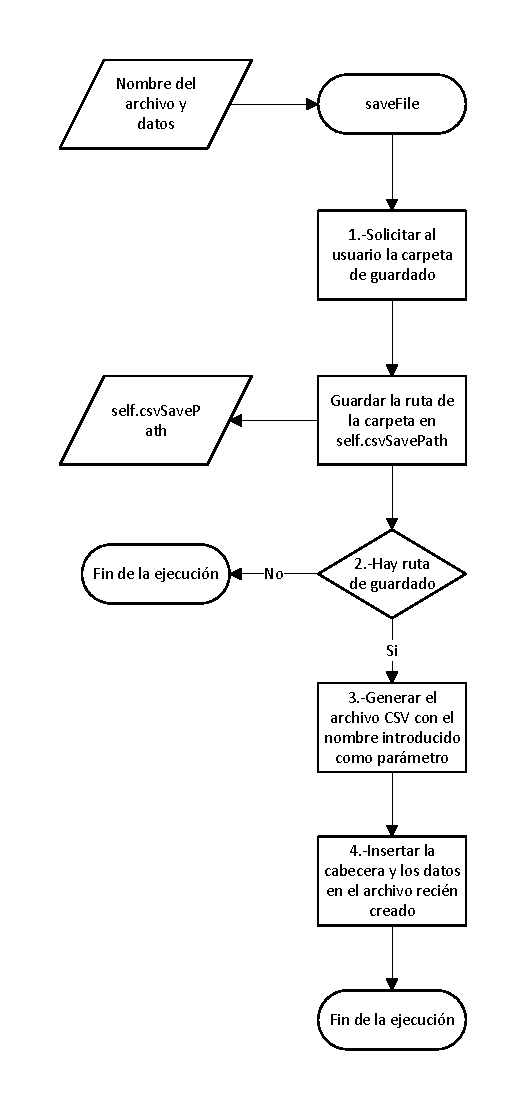
\includegraphics[width=.42\textwidth]{fig/Diagramas de flujo/saveFile-CSV.pdf}
\caption{Diagrama de flujo que muestra el proceso de generación de un archivo \acrshort{CSV} mediante \texttt{saveFile}.}
\label{fig:DiagramaFlujoSaveFileCsv}
\end{figure}

\begin{lstlisting}[language=Python,
                   style=python,
                   frame=none,
                   numbers=none,
                   basicstyle=\ttfamily\normalsize,
                   caption={Función \texttt{saveFile}},
                   label=src:functionCsvSaveFile,
                   inputencoding=utf8]                   
    def saveFile(self):
        try:
            self.getSavePath()
            # print(self.saveFilePath)
            if self.csvSavePath != "":
                with open(self.csvSavePath, 'w', encoding='utf-8') as file:
                    writer = self.csvWriter(file,delimiter=",",lineterminator="\n")
                    writer.writerow(self.columnsName)
                    writer.writerows(self.csvData)
        except Exception as e:
            print("Error: " + str(e))
        finally: del self
\end{lstlisting}

\subsubsection{Módulo de manejo de bases de datos}

El módulo \texttt{SQLHandler} se encarga de gestionar la comunicación con las tres bases de datos utilizadas por el software. Estas bases de datos almacenan los datos de la oferta y la demanda para las simulaciones, así como los resultados generados por el simulador.

El módulo consta de cuatro clases: tres destinadas a la gestión individual de cada una de las bases de datos (\texttt{SqlSupply}, \texttt{SqlDemand} y \texttt{SqlResults}), y una última enfocada a la verificación de las sentencias \acrshort{SQL} realizadas por los usuarios (\texttt{SqlTools}).

La clase \texttt{SqlSupply} es la encargada de gestionar la comunicación con la base de datos que almacena la información de los diferentes archivos de configuración de la oferta. Al utilizar esta clase, se genera una carpeta en el directorio de trabajo para almacenar la base de datos llamada "Database", si no existiera dicha carpeta, y dentro de esta, la base de datos con el nombre "supplyDb.db". Acto seguido, se genera una conexión con la base de datos para comenzar a construir la estructura de la misma. Esta estructura es la que se ha explicado en la Sección~\ref{subsec:dBSupply} y que aparece de manera simplificada en la Figura~\ref{fig:edrOfertaSimplificado} y de manera más detallada en el Anexo~\ref{fig:edrOferta}.

La creación de la base de datos comienza con la función \texttt{generateDataBaseTables}, que se encarga de ejecutar las subfunciones responsables de la creación de cada una de las tablas de la base de datos en un orden específico. El orden al generar las tablas es fundamental debido a que la creación de tablas con claves foráneas que referencien a otras requiere que las tablas referenciadas existan previamente. En caso contrario, la base de datos arrojará un error y esas tablas no se generarán. Debido a esto, primero se generan tablas que no contengan ninguna clave foránea y, después, se generan las tablas que contengan claves foráneas que apunten a tablas creadas con anterioridad. De esta forma se evitan errores durante la creación de la base de datos.

Las tablas se generan mediante una sentencia \acrshort{SQL}, en la que se definen todas las columnas que ha de tener la tabla, así como el tipo de datos que almacena cada una de estas columnas y las diferentes restricciones que se le pueden aplicar, como, por ejemplo, que los valores que contenga cada columna sean únicos, es decir, que esa columna no puede contener dos filas que tengan el mismo valor en esa columna. Un ejemplo de una de estas subfunciones podría ser \texttt{createServiceTable} (Listado~\ref{src:functionCreateServiceTable}), que genera la tabla \texttt{SERVICE} (Figura~\ref{fig:dbSupplySERVICE}). El diagrama de flujo de la Figura~\ref{fig:DiagramaFlujoCreateServiceTable} refleja el comportamiento de la función \texttt{createServiceTable}. La función \texttt{createServiceTable} sigue el siguiente proceso:
\begin{enumerate}
    \item \textit{Inicializar cursor:} Se inicializa el cursor encargado de realizar las tareas de ejecución y recuperación de resultados.
    \item \textit{Ejecutar sentencia \acrshort{SQL}:} Se comprueba que la tabla \texttt{SERVICE} no exista. Si la tabla no existe se ejecuta la sentencia \acrshort{SQL} que genera la tabla \texttt{SERVICE}, aplica las restricciones que tenga la tabla, en este caso, que cada fila sea única y se añaden las referencias a las distintas claves foráneas que existen en la tabla.
    \item \textit{Guardar los cambios:} Una vez ejecutada la sentencia \acrshort{SQL}, se guardan los cambios en la base de datos. Si la tabla existe se omite la ejecución de la sentencia \acrshort{SQL}.
    \item \textit{Cerrar el cursor:} Por último se cierra el cursor de la base de datos.
\end{enumerate}

\begin{figure}[H]
\centering
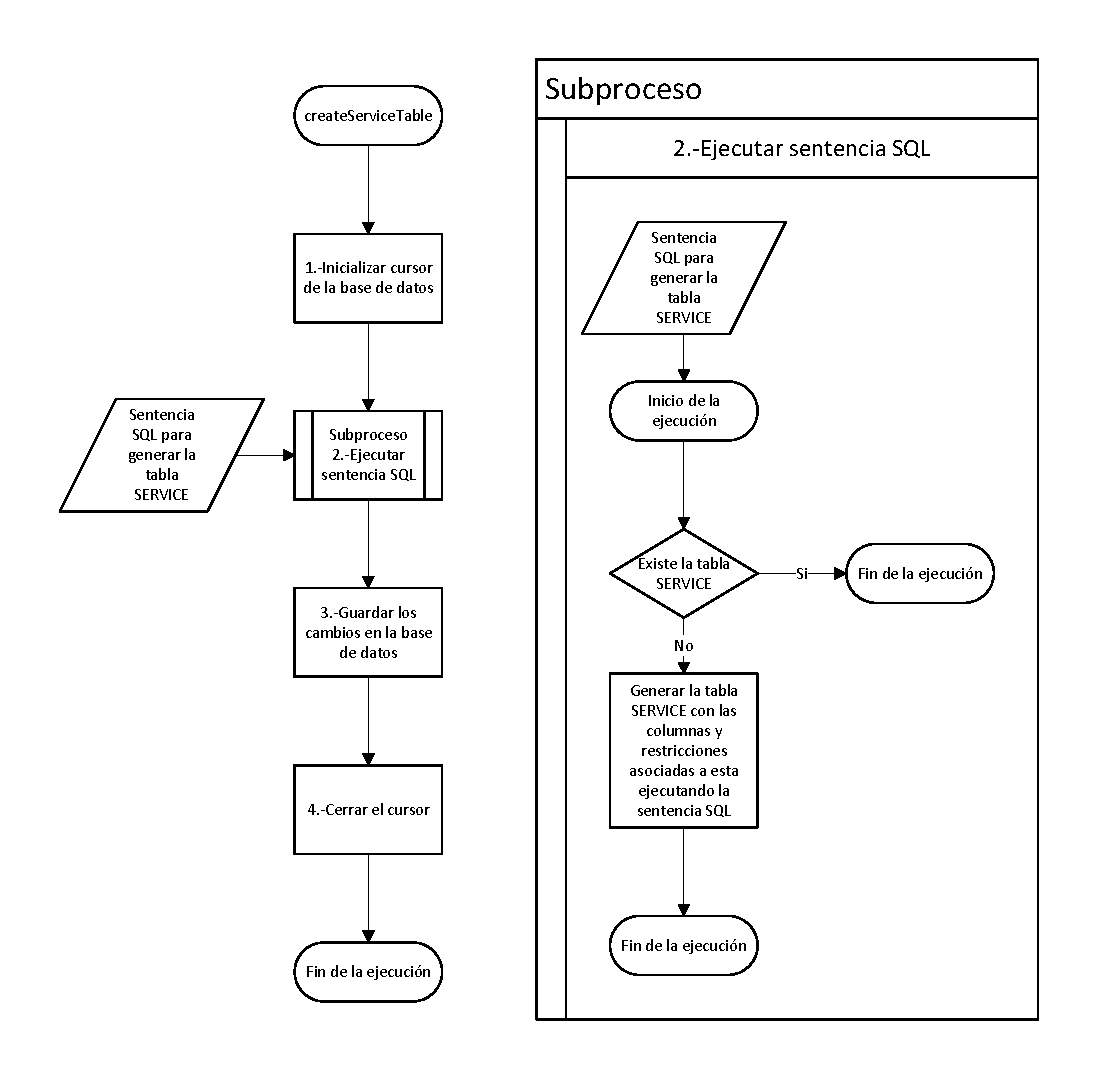
\includegraphics[width=.9\textwidth]{fig/Diagramas de flujo/createServiceTable.pdf}
\caption{Diagrama de flujo para la creación de la tabla \texttt{SERVICE}.}
\label{fig:DiagramaFlujoCreateServiceTable}
\end{figure}

\begin{lstlisting}[language=Python,
                   style=python,
                   frame=none,
                   numbers=none,
                   basicstyle=\ttfamily\normalsize,
                   caption={Función \texttt{createServiceTable}},
                   label=src:functionCreateServiceTable,
                   inputencoding=utf8]                   
def createServiceTable(self):
    """
    Genera la tabla SERVICE en la base de datos, si no existe
    :return:
    """
    self.initCursor()
    try:
        query = """CREATE TABLE IF NOT EXISTS SERVICE (
                    ID                        TEXT PRIMARY KEY,
            
                    DATE                      DATE,
                    
                    LINE                      TEXT REFERENCES LINE (ID) 
                                              ON DELETE CASCADE ON UPDATE CASCADE,
                                                                        
                    TRAIN_SERVICE_PROVIDER    TEXT REFERENCES TRAIN_SERVICE_PROVIDER (ID) 
                                              ON DELETE CASCADE ON UPDATE CASCADE,
                                                                                          
                    TIME_SLOT                 TEXT REFERENCES TIME_SLOT (ID) 
                                              ON DELETE CASCADE ON UPDATE CASCADE,
                                                                             
                    ROLLING_STOCK             TEXT REFERENCES ROLLING_STOCK (ID) 
                                              ON DELETE CASCADE ON UPDATE CASCADE,
                                                                                 
                    UNIQUE(ID,DATE,LINE,TRAIN_SERVICE_PROVIDER,TIME_SLOT,ROLLING_STOCK)
                    );"""
        self.cursor.execute(query)
        self.conector.commit()
    except sqlite3.Error as e:
        print(e)
    except Exception as e:
        print(e)
    except sqlite3.ProgrammingError as e:
        print(e)
    finally:
        self.cursor.close()
\end{lstlisting}

Las demás subfunciones tienen un comportamiento similar, variando en cada caso la sentencia \acrshort{SQL} para generar cada una de las tablas que componen la base de datos para los archivos de configuración de la oferta.

Dentro de la clase \texttt{SqlSupply} también se encuentran las funciones encargadas de insertar los datos en cada una de las tablas. Cada una de estas funciones ejecuta una sentencia \acrshort{SQL} para introducir los datos, pasados como parámetro a la función, a la tabla para la que esté diseñada dicha función. Estos datos deben ser una lista de listas, donde cada una de las listas corresponde a una fila dentro de la tabla, por lo que la sentencia se ejecuta tantas veces como elementos tenga la lista de listas en una misma transacción con la base de datos. Esto acelera el proceso de introducir los datos, ya que se realiza una única transacción, evitando que las sentencias se ejecuten de una en una. En caso de que exista un problema a la hora de procesar la transacción, se deshacen todos los cambios realizados en la tabla producidos durante la transacción. Un ejemplo de una de estas funciones podría ser la función que introduce los datos a la tabla \texttt{SERVICE}.

La función \texttt{insertServiceData} (Listado~\ref{src:functionInsertServiceData}) es la encargada de insertar los datos, que se le pasan como parámetro, a la tabla \texttt{SERVICE}. El funcionamiento de esta función se puede observar en el diagrama de flujo de la Figura~\ref{fig:diagramaFlujoInsertServiceData}. El procedimiento seguido por la función es:
    \begin{enumerate}
        \item \textit{Inicializar el cursor:} Se inicializa el cursor de la base de datos. Este permite ejecutar las sentencias \acrshort{SQL}.
        
        \item \textit{Generar la entrada:} Se genera una lista de listas donde cada una de las sublistas contiene los 6 primeros elementos de los datos introducidos como parámetro. Estos datos corresponden con las claves \texttt{id}, \texttt{date}, \texttt{line}, \texttt{train\_service\_provider}, \texttt{time\_slot} y \texttt{rolling\_stock} bajo la clave raíz \texttt{service}. Esta lista de listas está almacenada en la variable \texttt{inputData}.
        
        \item \textit{Insertar datos:} Se ejecuta la sentencia \acrshort{SQL} para introducir los datos de \texttt{inputData} en la tabla \texttt{SERVICE} de la base de datos de los archivos de entrada de datos de la oferta. La sentencia \acrshort{SQL} se ejecuta tantas veces como sublistas existan dentro de la lista de listas almacenada en \texttt{inputData}. Esto inserta una fila en la tabla cada vez que se ejecuta la sentencia \acrshort{SQL} dentro de la transacción.

        \item \textit{Confirmar cambios:} Se confirman los cambios realizados en la tabla \texttt{SERVICE}, en este caso, la inserción de los datos pasados como parámetros a la función.
        
        \item \textit{Cerrar el cursor:} Por último se cierra el cursor de la base de datos.
    \end{enumerate}

\begin{figure}[H]
\centering
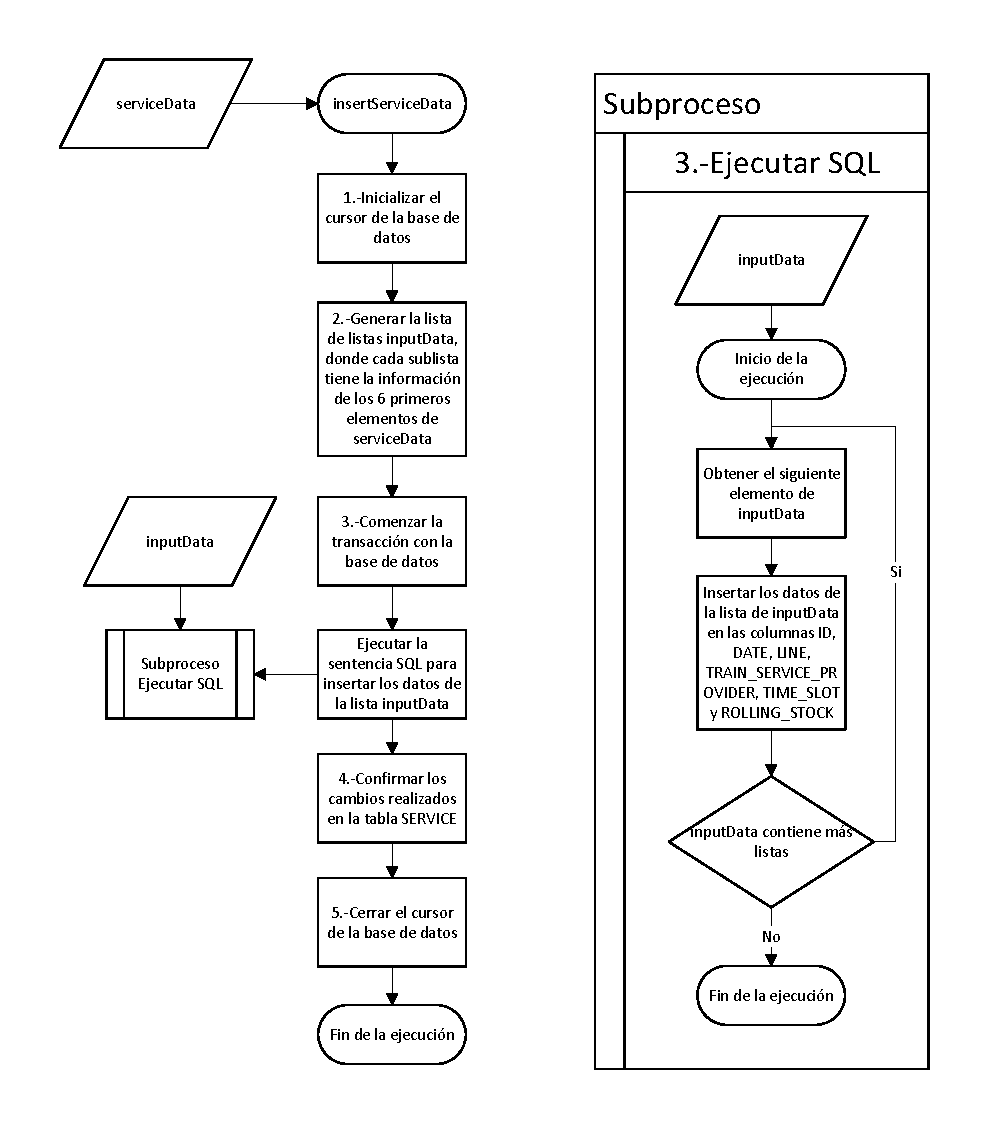
\includegraphics[width=.9\textwidth]{fig/Diagramas de flujo/insertServiceData.pdf}
\caption{Diagrama de flujo de la función \texttt{insertServiceData} }
\label{fig:diagramaFlujoInsertServiceData}
\end{figure}

%La función \texttt{insertServiceData} (Listado~\ref{src:functionInsertServiceData}) es la encargada de insertar los datos en la tabla \texttt{SERVICE}. Esto se hace empleando la sentencia \acrshort{SQL} almacenada en la variable \texttt{query} dentro de la función. Esta sentencia es única para cada una de las tablas. Esto se debe a que cada tabla tiene una estructura diferente y ha de especificarse en qué columnas hay que almacenar cada uno de los elementos de la lista que compone la fila dentro de la tabla. Para comenzar la transacción, se ejecuta la sentencia \acrshort{SQL} \texttt{BEGIN TRANSACTION} y, mediante la función \texttt{self.cursor.executemany(query, inputData)} se ejecuta la sentencia almacenada en la variable \texttt{query} tantas veces como elementos tenga la variable \texttt{inputData}. Después, para que los cambios sean registrados en la tabla, se hace uso de \texttt{self.conector.commit()} que manda la orden a la base de datos para que haga efectivos los cambios realizados en la última transacción. Si en algún punto del proceso descrito hubiera algún error, la base de datos desharía los cambios realizados en la última transacción empleando \texttt{self.conector.rollback()}. Por último, se cierra el cursor de la base de datos. Este comportamiento puede observarse en el diagrama de flujo de la Figura~\ref{fig:diagramaFlujoInsertServiceData}

\begin{lstlisting}[language=Python,
                   style=python,
                   frame=none,
                   numbers=none,
                   basicstyle=\ttfamily\normalsize,
                   caption={Función \texttt{insertServiceData}},
                   label=src:functionInsertServiceData,
                   inputencoding=utf8]                   
def insertServiceData(self, serviceData):
    """
    Inserta los datos de los servicios en la tabla SERVICE
    :param serviceData: Datos de los servicios
    :return:
    """
    self.initCursor()
    try:
        inputData = [service[:6]
                     for service in serviceData]
        query = "INSERT OR IGNORE INTO SERVICE (ID,DATE,LINE,TRAIN_SERVICE_PROVIDER,TIME_SLOT,ROLLING_STOCK) VALUES (?,?,?,?,?,?)"
        self.cursor.execute("BEGIN TRANSACTION")
        self.cursor.executemany(query, inputData)
        self.conector.commit()
    except sqlite3.Error as e:
        print("Service Sqlite Error SERVICE: "+str(e))
        self.conector.rollback()
    except Exception as e:
        print("Service Error: "+str(e))
        self.conector.rollback()
    except sqlite3.ProgrammingError as e:
        print("Service Sqlite programming Error: "+str(e))
        self.conector.rollback()
    finally:
        self.cursor.close()
\end{lstlisting}

Las otras funciones encargadas de insertar la información en las tablas de la base de datos siguen la misma dinámica que \texttt{insertServiceData}, pero cada una tiene una sentencia \acrshort{SQL} similar, variando en cada caso la tabla en la que se quiere introducir la información y las columnas que van a almacenar dicha información.

En la clase \texttt{SqlSupply}, también se pueden encontrar las funciones encargadas de borrar los archivos y los datos asociados a estos. Empleando la función \texttt{deleteTestEntry} (Listado~\ref{src:functionDeleteTestEntry}) se eliminan los archivos de una lista pasada como parámetro a la función. Además, esta función ejecuta una serie de subfunciones para eliminar la información que pueda permanecer en las tablas de la base de datos y que ya no tenga ningún test asociado, apoyándose en las tablas auxiliares para tal fin.

%Una de las funciones encargadas de eliminar elementos que ya no tengan ningún test asociado es, por ejemplo, \texttt{deleteUnusedServiceData} (Listado~\ref{src:functionDeleteUnusedServiceData}). Esta función buscará qué elementos no estén presentes en la tabla auxiliar \texttt{AUX\_SERVICE} (Figura~\ref{fig:dbSupplyAUX_SERVICE}) pero que sí se encuentren en la tabla \texttt{SERVICE} (Figura~\ref{fig:dbSupplySERVICE}) y los eliminará de la tabla \texttt{SERVICE}. Todas las tablas que contengan datos que contengan una referencia con la tabla \texttt{SERVICE} mediante una clave foránea también eliminarán las entradas que contengan los datos que hagan referencia a las entradas que se han eliminado. De esta manera, las tablas \texttt{RESTRICTIONS} y \texttt{ORIGIN\_DESTINATION\_TUPLES} eliminarán cualquier fila que comparta en las columnas \texttt{SERVICE\_ID} los mismos identificadores que se hayan eliminado de la tabla \texttt{SERVICE}. Este comportamiento sigue el diagrama de flujo de la Figura~\ref{fig:diagramaFlujoDeleteUnusedServiceData}

Una de las funciones encargadas de eliminar elementos que ya no tengan ningún archivo asociado es, por ejemplo, \texttt{deleteUnusedServiceData} (Listado~\ref{src:functionDeleteUnusedServiceData}). Esta función ejecuta una sentencia \acrshort{SQL} que busca y elimina elementos huérfanos dentro de la base de datos destinada a archivos de entrada de datos de la oferta. El comportamiento de la función puede verse en el diagrama de flujo de la Figura~\ref{fig:diagramaFlujoDeleteUnusedServiceData}. El proceso que sigue esta función es el siguiente:
    \begin{enumerate}
        \item \textit{Ejecución de la sentencia \acrshort{SQL}:} La función comienza la ejecución de la sentencia \acrshort{SQL}.
        \item \textit{Selección de los servicios:} La base de datos busca todos los identificadores pertenecientes a los servicios dentro de la tabla \texttt{SERVICE}.
        \item \textit{Comprobar pertenencia:} Se comprueba que los identificadores recopilados en el paso anterior tengan asociados uno o más archivos. Esto se hace buscando en la tabla auxiliar \texttt{AUX\_SERVICE} que todos los identificadores de los servicios recopilados anteriormente se encuentren presentes, ya que si se encuentran en dicha tabla, significa que tienen asociado mínimo un archivo. En caso de que existan elementos dentro de la tabla \texttt{SERVICE} que no tengan asociado un archivo, es decir, que no aparezcan en la tabla \texttt{AUX\_SERVICE}, estos se eliminan de la tabla \texttt{SERVICE}. En el caso contrario, el programa para la ejecución sin realizar ningún cambio en la tabla \texttt{SERVICE}.
    \end{enumerate}

\begin{figure}[H]
\centering
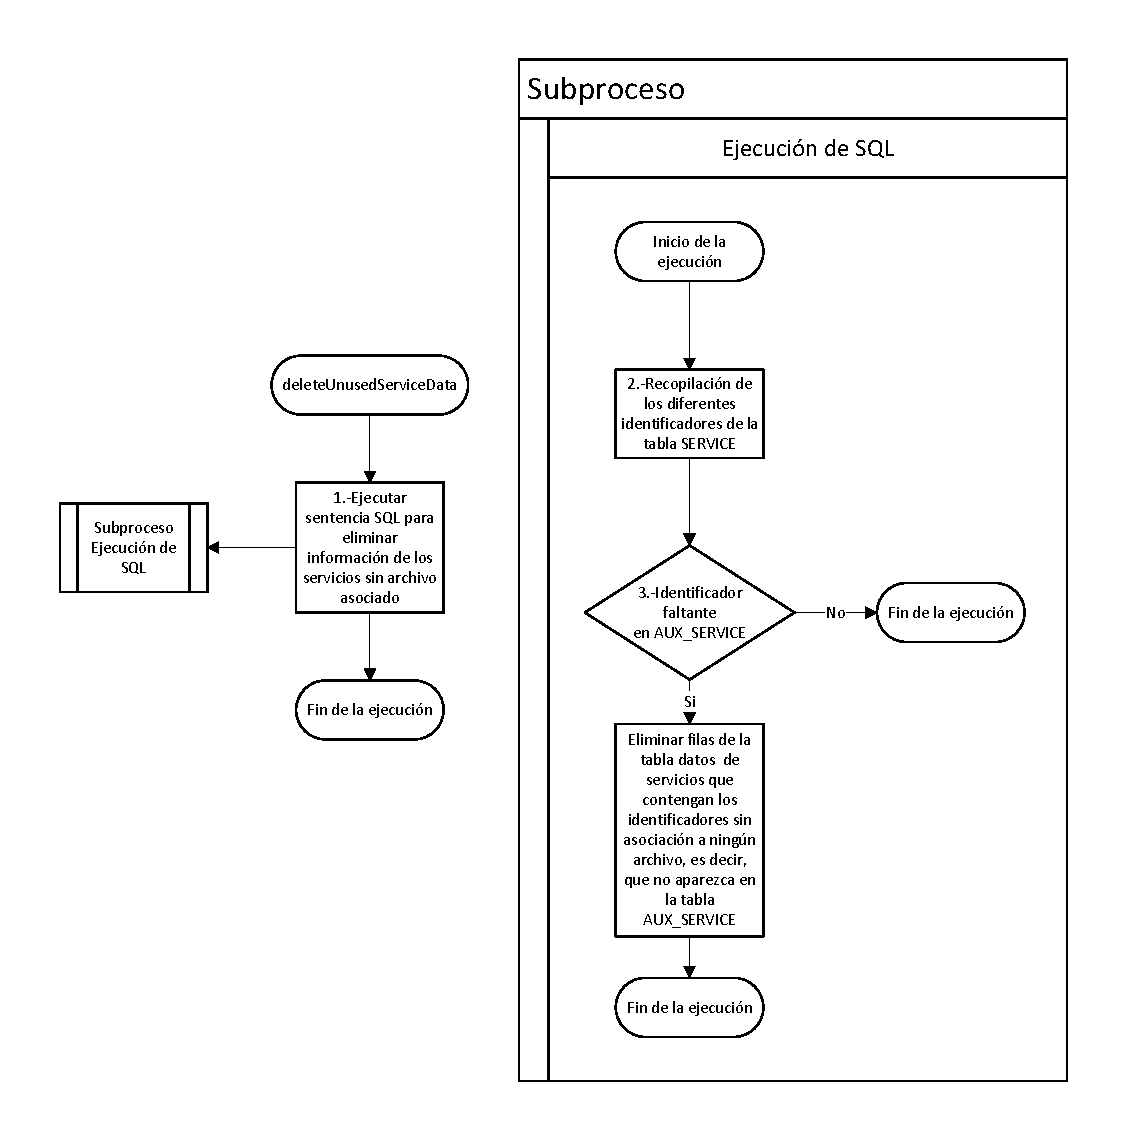
\includegraphics[width=.9\textwidth]{fig/Diagramas de flujo/deleteUnusedServiceData.pdf}
\caption{Diagrama de flujo de la función \texttt{deleteUnusedServiceData} }
\label{fig:diagramaFlujoDeleteUnusedServiceData}
\end{figure}

\begin{lstlisting}[language=Python,
                   style=python,
                   frame=none,
                   numbers=none,
                   basicstyle=\ttfamily\normalsize,
                   caption={Función \texttt{deleteTestEntry}},
                   label=src:functionDeleteTestEntry,
                   inputencoding=utf8]                   
def deleteTestEntry(self, testList):
    """
    Borra un test elegido por el usuario y todos los datos relacionados con este. Si los datos son comunes a otros
    tests, estos datos no se eliminarán.
    :return:
    """
    try:
        self.initCursor()
        for testName in testList:
            query = f"""DELETE FROM TESTS WHERE TESTS.NAME = '{testName}'"""
            self.cursor.execute(query)

        self.conector.commit()

        self.deleteUnusedSeatData()
        self.deleteUnusedServiceData()
        self.deleteUnusedCorridorData()
        self.deleteUnusedStationsData()
        self.deleteUnusedTrainServiceProviderData()
        self.deleteUnusedTimeSlotData()
        self.deleteUnusedRollingStockData()

    except sqlite3.Error as e:
        print("Sqlite Error: " + str(e))
    except EmptyTestData as e:
        print(e)
    except Exception as e:
        print(e)
    except sqlite3.ProgrammingError as e:
        print(e)
    finally:
        self.cursor.close()
\end{lstlisting}

\begin{lstlisting}[language=Python,
                   style=python,
                   frame=none,
                   numbers=none,
                   basicstyle=\ttfamily\normalsize,
                   caption={Función \texttt{deleteUnusedServiceData}},
                   label=src:functionDeleteUnusedServiceData,
                   inputencoding=utf8]                   
def deleteUnusedServiceData(self):
    """
    Borra todos los datos que no se estén utilizando por ningún test en la tabla SERVICE
    :return:
    """
    try:
        query = f"""DELETE FROM SERVICE
                    WHERE SERVICE.ID NOT IN (
                    SELECT AUX_SERVICE.SERVICE_ID FROM AUX_SERVICE)"""
        self.cursor.execute(query)
        self.conector.commit()

    except sqlite3.Error as e:
        print("Sqlite Error: " + str(e))
    except Exception as e:
        print(e)
    except sqlite3.ProgrammingError as e:
        print(e)
\end{lstlisting}

La clase \texttt{SqlSupply} también posee funciones que extraen los datos de la base de datos para, posteriormente, reconstruir el archivo de entrada de datos de la oferta. Estas funciones convierten los datos extraídos al mismo formato que adoptan los archivos \acrshort{Yaml} al ser cargados en Python mediante la librería PyYaml~\cite{PyYaml}, es decir, un diccionario.  

La función principal para la extracción de los datos y posterior construcción del diccionario para recrear el archivo \acrshort{Yaml} es \texttt{getDataForDumpYaml} (Listado~\ref{src:functionGetDataForDumpYaml}), que toma como parámetro el nombre del archivo que se va a reconstruir. Este nombre se emplea posteriormente por las subfunciones encargadas de reconstruir la información de cada una de las claves raíz que aparecen en los archivos de configuración de la oferta para extraer los datos que correspondan a ese test.

\begin{lstlisting}[language=Python,
                   style=python,
                   frame=none,
                   numbers=none,
                   basicstyle=\ttfamily\normalsize,
                   caption={Función \texttt{getDataForDumpYaml}},
                   label=src:functionGetDataForDumpYaml,
                   inputencoding=utf8]                   
def getDataForDumpYaml(self,testName):
    """
    Genera la estructra necesaria para reconstruir el archivo de oferta mediante subfunciones para cada
    uno de los apartados dentro del archivo yaml.
    :return: testName, data
    """
    data = {}
    try:
        self.initCursor()

        data.update(self.getDataForStations(testName))
        data.update(self.getDataForSeat(testName))
        data.update(self.getDataForCorridor(testName))
        data.update(self.getDataForLine(testName))
        data.update(self.getDataForRollingStock(testName))
        data.update(self.getDataForTrainServiceProvider(testName))
        data.update(self.getDataForTimeSlot(testName))
        data.update(self.getDataForService(testName))

    except sqlite3.Error as e:
        print("Sqlite Error: " + str(e))
    except Exception as e:
        print(e)
    except sqlite3.ProgrammingError as e:
        print(e)
    finally:
        self.cursor.close()
        return data
\end{lstlisting}

Una de las subfunciones encargadas de reconstruir la información de las claves raíz es la función \texttt{getDataForTimeSlot} (Listado~\ref{src:functionGetDataForTimeSlot}). El comportamiento de esta función se muestra en el diagrama de flujo de la Figura~\ref{fig:diagramaFlujoGetDataForTimeSlot}. El procedimiento seguido por la función es:
    \begin{enumerate}
        \item \textit{Ejecución de sentencia \acrshort{SQL}:} Se ejecuta la sentencia que, teniendo el nombre del archivo del archivo que se quiere regenerar, obtiene todos los datos asociados a este mediante la tabla auxiliar \texttt{AUX\_TIME\_SLOT}. Con esta tabla, se obtienen los identificadores de los datos de la tabla \texttt{TIME\_SLOT} que pertenecen al archivo. Se extraen las filas que contengan dichos identificadores y se ordenan de manera ascendente por el valor del identificador.
        \item \textit{Recolección de datos:} Se recogen los datos seleccionados por la base de datos en el paso anterior. Estos datos están almacenados en una lista de tuplas, donde cada tupla corresponde con una fila de los datos seleccionados con la sentencia \acrshort{SQL}.
        \item \textit{Construcción de salida:} Con los datos obtenidos, se construye una lista de diccionarios donde cada diccionario posee las claves \texttt{id}, \texttt{start} y \texttt{end}, corresponden con los elementos 0, 1 y 2 de cada una de las tuplas que conforman la lista de tuplas con los datos extraidos de la base de datos. Posteriormente, esta lista de diccionarios se añade a un diccionario bajo la clave \texttt{timeSlot}, que es una de las claves raíz del archivo de entrada de datos de la oferta.
        \item \textit{Retorno de salida con formato:} Una vez construido el diccionario con los datos solicitados a la base de datos, este se devuelve y, por ende, finaliza la ejecución de la función.
    \end{enumerate}


%Esta función emplea una sentencia \acrshort{SQL} para seleccionar los datos de la tabla \texttt{TIME\_SLOT} que pertenecen al archivo, cuyo nombre se ha pasado como argumento de la función. Esta sentencia emplea las relaciones entre las tablas \texttt{TESTS} (Figura~\ref{fig:dbSupplyTESTS}) y \texttt{AUX\_TIME\_SLOT} (Figura~\ref{fig:dbSupplyAUX_TIME_SLOT}) para extraer todos los identificadores de los intervalos de tiempo de llegada y salida de los trenes de una estación. Los identificadores se emplean para seleccionar la información de la tabla \texttt{TIME\_SLOT} que contenga dichos identificadores en su columna \texttt{ID}. Esta sentencia devuelve una lista de tuplas, donde cada una de estas tuplas representa una fila de la tabla \texttt{TIME\_SLOT}. Haciendo uso de esta lista de tuplas, se reconstruye la estructura que tiene la información en el archivo \acrshort{Yaml}, es decir, una lista de diccionarios donde cada diccionario posee las claves \texttt{id}, \texttt{start} y \texttt{end} siendo los valores de estas claves los correspondientes a los elementos con índice 0, 1 y 2 en la tupla que contiene los datos de una fila. Por último, esta lista de diccionarios se añade a un diccionario que contiene la clave raíz \texttt{timeSlot} el cual se devuelve. Este diccionario se emplea por la función \texttt{getDataForDumpYaml} para reconstruir el diccionario que contiene toda la información del archivo de entrada de datos de la oferta al que pertenezcan esos datos. El funcionamiento de la función puede verse en la Figura~\ref{fig:diagramaFlujoGetDataForTimeSlot}.

\begin{figure}[H]
\centering
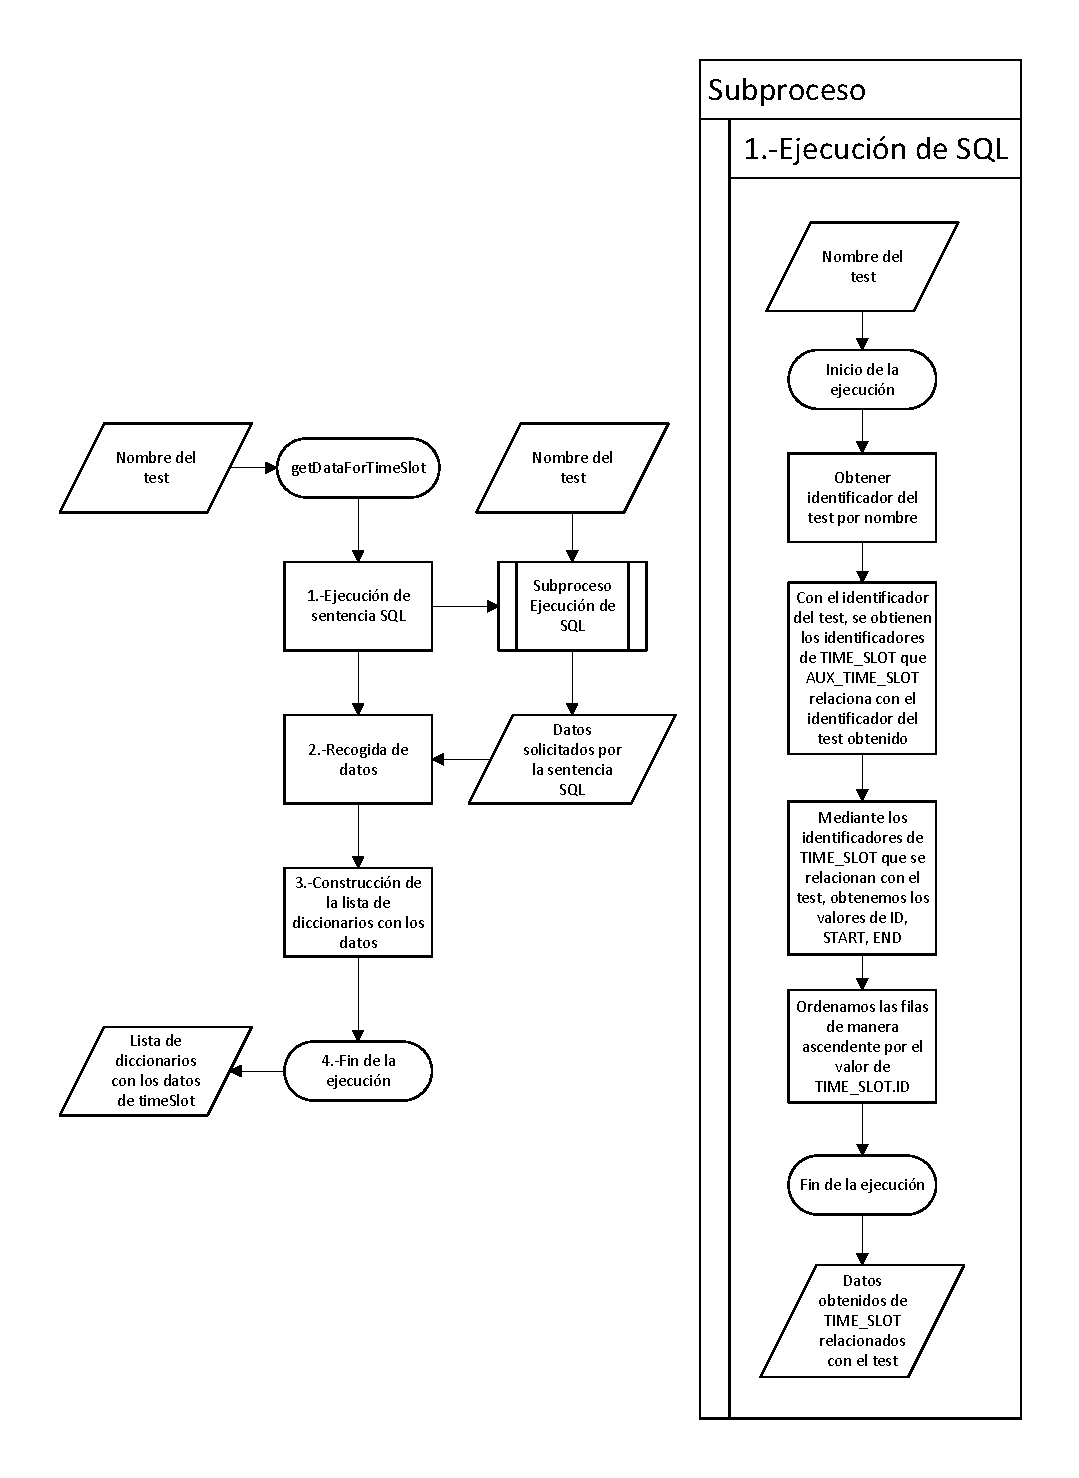
\includegraphics[width=.85\textwidth]{fig/Diagramas de flujo/getDataForTimeSlot.pdf}
\caption{Diagrama de flujo de la función \texttt{getDataForTimeSlot}}
\label{fig:diagramaFlujoGetDataForTimeSlot}
\end{figure}

\begin{lstlisting}[language=Python,
                   style=python,
                   frame=none,
                   numbers=none,
                   basicstyle=\ttfamily\normalsize,
                   caption={Función \texttt{getDataForTimeSlot}},
                   label=src:functionGetDataForTimeSlot,
                   inputencoding=utf8]                   
def getDataForTimeSlot(self, testName):
    """
    Obtiene los datos de los slots de tiempo y los formatea para que sigan la estructra de timeSlot dentro del archivo
    yaml de la oferta
    :param testName: Nombre del test que se está extrayendo
    :return:
    """
    try:
        query = f"""SELECT 
                        TIME_SLOT.ID,
                        TIME_SLOT.START,
                        TIME_SLOT.END                            
                    FROM 
                        TIME_SLOT
                    WHERE TIME_SLOT.ID IN (
                        SELECT AUX_TIME_SLOT.TIME_SLOT_ID FROM AUX_TIME_SLOT
                        INNER JOIN TESTS ON TESTS.ID = AUX_TIME_SLOT.TEST_ID
                        WHERE TESTS.NAME = '{testName}')
                    ORDER BY TIME_SLOT.START ASC"""

        self.cursor.execute(query)
        data = self.cursor.fetchall()
        formatedData = [{"id": element[0],"start": element[1],"end": element[2]}
                        for element in data]
        outputData = {"timeSlot": formatedData}
        return outputData
    except sqlite3.Error as e:
        print("Sqlite Error: " + str(e))
    except Exception as e:
        print(e)
    except sqlite3.ProgrammingError as e:
        print(e)
\end{lstlisting}

En esta clase \texttt{SqlSupply} también se encuentra la función \texttt{executeQuery} (Listado~\ref{src:functionExecuteQuery}) encargada de ejecutar las sentencias, que se pasan como parámetro, en la base de datos para los archivos de la oferta. Esta función puede ejecutar cualquier sentencia válida en la base de datos. Si esta sentencia selecciona datos empleando el comando \texttt{SELECT}, la función devuelve los nombres de las columnas que han sido seleccionadas, así como la información contenida que cumpla con las especificaciones introducidas en la sentencia. Un ejemplo de esto puede ser el uso de la sentencia \texttt{SELECT ID, NAME FROM STATIONS}. Esta sentencia devuelve el identificador y el nombre de cada una de las estaciones que se encuentren en la tabla \texttt{STATIONS} (Figura~\ref{fig:dbSupplySTATIONS}) por lo que el valor de la variable \texttt{cols} es una lista con los nombres \texttt{ID} y \texttt{NAME}, que corresponden a los nombres de las columnas de las que se quieren obtener datos, mientras que la variable \texttt{result} contiene una lista de tuplas donde cada una de las tuplas sería una fila de la base de datos con dos elementos: el identificador de la estación y el nombre que recibe la misma.

\begin{lstlisting}[language=Python,
                   style=python,
                   frame=none,
                   numbers=none,
                   basicstyle=\ttfamily\normalsize,
                   caption={Función \texttt{executeQuery}},
                   label=src:functionExecuteQuery,
                   inputencoding=utf8]                   
def executeQuery(self,query):
    try:
        self.initCursor()
        self.cursor.execute(query)
        self.conector.commit()

        strippedQuery = query.strip().upper()

        if strippedQuery.startswith("SELECT"):
            cols = [item[0] for item in self.cursor.description]
            result = self.cursor.fetchall()
            return cols,result

    except sqlite3.Error as e:
        print(e)
        return -1
    except Exception as e:
        print(e)
        return -1
    except sqlite3.ProgrammingError as e:
        print(e)
        return -1
    finally:
        self.cursor.close()
\end{lstlisting}

En cuanto a las clases \texttt{SqlDemand} y \texttt{SqlResults}, estas contienen funciones que realizan las mismas tareas que las descritas en la clase \texttt{SqlSupply}, es decir, crear las tablas que conforman las bases de datos para los archivos de entrada de datos de la demanda y para los archivos de resultados de las simulaciones, insertar datos en dichas tablas, eliminar archivos de las bases de datos y ejecutar sentencias \acrshort{SQL} en sus respectivas bases de datos. Dichas funciones están adaptadas a cada base de datos, en el caso de las funciones dentro de la clase \texttt{SqlDemand}, están adaptadas para funcionar con la base de datos que almacena los datos de los archivos de entrada de datos de la demanda y en el caso de las funciones dentro de la clase \texttt{SqlResults}, están adaptadas para funcionar con la base de datos cuyo propósito es el de almacenar los resultados de las diferentes simulaciones que se realicen con el simulador. 

Por último, la clase \texttt{SqlTools} (Listado~\ref{src:classSqlTools}) posee funciones cuyo cometido es el de validar las sentencias antes de que se ejecuten en las bases de datos, evitando la ejecución de aquellas que contengan errores. Esta clase contiene dos funciones:
\begin{itemize}
    \item La función \texttt{validateSyntaxQuery} está destinada a validar la sintaxis de la sentencia utilizando el comando SQL \texttt{EXPLAIN}, el cual permite obtener el plan de ejecución sin ejecutar realmente los comandos, en una base de datos temporal en memoria que se encuentra vacía.
    \item La función \texttt{validateQueryOnDb} se encarga de validar la sentencia en la base de datos donde se va a ejecutar, con el fin de evitar errores que no sean de sintaxis, como por ejemplo, que una de las columnas mencionadas en la sentencia no existe. Esta función también emplea el comando \texttt{EXPLAIN} para llevar a cabo la validación.
\end{itemize}


\begin{lstlisting}[language=Python,
                   style=python,
                   frame=none,
                   numbers=none,
                   basicstyle=\ttfamily\normalsize,
                   caption={Clase \texttt{SqlTools}},
                   label=src:classSqlTools,
                   inputencoding=utf8]                   
class SqlTools:
    def __init__(self):
        self.connector = sqlite3.connect(":memory:")

    def validateSyntaxQuery(self,query):
        try:
            self.connector.execute(f"EXPLAIN QUERY PLAN {query}")
            return True

        except sqlite3.OperationalError as e:
            if "no such table" in str(e):
                return True
            else:
                print(e)
                return False
        except sqlite3.Error as e:
            print(f"Query invalida: {e}")
            return False

    def validateQueryOnDb(self,query,conn):
        try:
            conn.execute(f"EXPLAIN QUERY PLAN {query}")
            return True, ""

        except sqlite3.OperationalError as e:
            print(f"Query invalida: {e}")
            return False, str(e)
        except sqlite3.Error as e:
            print(f"Query invalida: {e}")
            return False , str(e)
\end{lstlisting}

\subsubsection{Módulo de introducción de datos}

El módulo \texttt{dataLoger} está enfocado a introducir los datos de los diferentes archivos dentro de la base de datos, empleando para ello las funciones de los módulos \texttt{yamlParser} y \texttt{SQLHandler}. Este módulo contiene una clase dedicada a introducir la información dentro de cada base de datos manejada por la aplicación, una para la base de datos de los archivos de entrada de datos de la oferta, otra para la base de datos de los archivos de entrada de datos de la demanda y otra para la base de datos de los archivos de resultados arrojados por el simulador.

Cada una de las clases que componen este módulo posee una función principal desde la cual se ejecutan todas las demás funciones encargadas de añadir la información a las bases de datos. Estas subfunciones emplean funciones del módulo encargado de la comunicación con las bases de datos para insertar los datos de cada uno de los archivos en su correspondiente tabla dentro de la base de datos diseñada para ese archivo.

Un ejemplo de estas subfunciones es la función \texttt{logStationData}. Esta función primero extrae los datos de la clave raíz \texttt{stations} empleando la función \texttt{getStationsData} perteneciente a la clase \texttt{Parser} del módulo \texttt{yamlParser}. 

Una vez obtenidos los datos de la clave raíz \texttt{stations} se emplean las funciones destinadas a introducir los datos en la base de datos, en este caso, en la tabla \texttt{STATIONS} de la base de datos de los archivos de entrada de datos de la oferta, que se encuentran en la clase \texttt{SqlSupply} dentro del módulo \texttt{SQLHandler}. 

\begin{lstlisting}[language=Python,
                   style=python,
                   frame=none,
                   numbers=none,
                   basicstyle=\ttfamily\normalsize,
                   caption={Función \texttt{logStationData}},
                   label=src:functionLogStationData,
                   inputencoding=utf8]                   
def logStationsData(self):
    """
    Introduce los datos de las estaciones a la base de datos de la oferta
    :return:
    """ 
    
    data = self.yml.getStationsData()
    self.sqlSupply.insertStationsData(data)
    self.sqlSupply.insertAuxStationsData(data, self.testID)
\end{lstlisting}

\subsubsection{Módulo de configuración}

El módulo \texttt{configManager} se encarga de gestionar la configuración del programa, concretamente, de las sentencias \acrshort{SQL} almacenadas para su uso posterior. Estas sentencias se guardan en un archivo \acrshort{JSON}. 

El archivo de configuración se genera en la carpeta \texttt{config}, ubicada dentro del directorio de trabajo del programa, con el nombre \texttt{config.json}. Tanto el directorio como el archivo se crean automáticamente al iniciar la aplicación por primera vez o si, al arrancarla, el archivo no existe. Este comportamiento se define en la generación de la clase \texttt{Config} dentro del módulo \texttt{configManager}.

Por defecto, el archivo de configuración se genera con un conjunto de sentencias diseñado para mostrar los archivos almacenados en cada base de datos. Estas sentencias se guardan bajo la clave \texttt{SQL\_Querys} dentro de una lista de diccionarios. Las claves de estos diccionarios corresponden al nombre asignado a cada sentencia en el archivo de configuración, y su valor es otro diccionario que contiene dos claves: \texttt{db} y \texttt{query}, las cuales indican la base de datos en la que se ejecutará la sentencia y la propia sentencia a ejecutar, respectivamente.

Esto se realiza mediante la función \texttt{generateDefaultConfig} (Listado~\ref{src:functionGenerateDefaultConfig}).

\begin{lstlisting}[language=Python,
                   style=python,
                   frame=none,
                   numbers=none,
                   basicstyle=\ttfamily\normalsize,
                   caption={Función \texttt{generateDefaultConfig}},
                   label=src:functionGenerateDefaultConfig,
                   inputencoding=utf8]                   
def generateDefaultConfig(self):
    """
    Esta funcion genera la configuracion inicial para la aplicacion, la cual contiene querys de SQL utiles
    y bastante usadas en las bases de datos que maneja el programa.
    :return: None
    """
    try:
        data = {
            'SQL_Querys':{
                "Mostrar test de oferta":{"db":"oferta","query":"SELECT * FROM TESTS"},
                "Mostrar test de demanda": {"db": "demanda", "query": "SELECT * FROM TESTS"},
                "Mostrar test de resultados": {"db": "resultados", "query": "SELECT * FROM TESTS"}
            }
        }
        self.configData = deepcopy(data)
        with open(self.configFilePath,'w') as configFile:
            json.dump(data,configFile,indent=4)
    except Exception as e:
        print(e)
\end{lstlisting}

Mediante el uso de \texttt{addSQLQuery} (Listado~\ref{src:functionAddSqlQuery}) se pueden agregar sentencias al archivo de configuración. Esta función tomará como parámetros el nombre que recibe la sentencia \acrshort{SQL}, que servirá como clave dentro del diccionario que almacena las sentencias, la base de datos en la que se ejecutará la sentencia y la sentencia \acrshort{SQL} en sí. Con estos parámetros se genera una entrada dentro del diccionario y se introduce una clave nueva, que corresponde con el nombre que se ha pasado como argumento y, bajo esta clave, se genera otro diccionario con las claves "db" y "query", donde se guardan la base de datos donde se va a ejecutar la sentencia y la sentencia \acrshort{SQL} respectivamente.

\begin{lstlisting}[language=Python,
                   style=python,
                   frame=none,
                   numbers=none,
                   basicstyle=\ttfamily\normalsize,
                   caption={Función \texttt{addSQLQuery}},
                   label=src:functionAddSqlQuery,
                   inputencoding=utf8]                   
def addSQLQuery(self,name,db,query):
    """
    Esta funcion se encarga de agregar querys de SQL a la lista almacenada en el archivo de configuracion
    :return: None
    """
    try:
        self.configData["SQL_Querys"].update({str(name):{"db":str(db),"query":str(query)}})
        self.saveConfig()
    except Exception as e: print(e)
\end{lstlisting}

De igual modo, usando la función \texttt{removeSQLQuery} (Listado~\ref{src:functionRemoveSqlQuery}) se eliminan sentencias \acrshort{SQL} que se encuentran ya almacenadas en el archivo de configuración. Para ello, esta función se vale del nombre que se le ha asignado a la sentencia \acrshort{SQL} para eliminar la entrada que contiene la sentencia \acrshort{SQL} dentro del archivo de configuración.

\begin{lstlisting}[language=Python,
                   style=python,
                   frame=none,
                   numbers=none,
                   basicstyle=\ttfamily\normalsize,
                   caption={Función \texttt{removeSQLQuery}},
                   label=src:functionRemoveSqlQuery,
                   inputencoding=utf8]                   
def removeSQLQuery(self,name):
    """
    Esta funcion se encarga de eliminar querys de SQL a la lista almacenada en el archivo de configuracion
    :return: None
    """
    try:
        self.configData["SQL_Querys"].pop(name)
        self.saveConfig()
    except Exception as e: print(e)
\end{lstlisting}

\subsection{Interfaz gráfica}

Para construir la interfaz gráfica del programa se ha empleado el paquete Tkinter~\cite{Tkinter} incluido en Python. Este paquete actúa como una envoltura sobre la biblioteca Tcl/Tk, escrita en C, permitiendo a Python comunicarse con el intérprete \acrfull{Tcl} mediante el módulo interno \texttt{\_tkinter}. Cuando se emplea Tkinter, lo que realmente ocurre es que Python genera una cadena de comandos \acrshort{Tcl}, que mediante el intérprete de Tcl, invoca a las funciones del sistema gráfico a través de Tk o Ttk. Estos gestionan directamente los elementos de la interfaz a través del sistema gráfico del sistema operativo.

Tkinter es multiplataforma, es decir, puede funcionar en varios sistemas operativos sin necesidad de cambiar el código, en la mayoría de las ocasiones, ya que se encuentra implementado sobre \acrfull{API} nativas de cada sistema operativo, \acrfull{GDI} y USER32 para sistemas con Windows, Cocoa o Quartz para sistemas con MacOS y X11 para sistemas Linux/Unix.

A continuación, se desarrollará una explicación de algunos de los elementos de Tkinter empleados en la construcción de la interfaz para la aplicación que gestiona el flujo de datos entre los archivos y las bases de datos que componen este \acrshort{TFG}, apoyándose en un programa de ejemplo que contiene un contador y un generador de ventanas de mensajes. Esto se ha decidido así debido a que el entorno tiene muchos más elementos que complicarían la explicación, mientras que con un ejemplo más sencillo se puede entender el funcionamiento de Tkinter y cómo se insertan y manejan los diferentes elementos.

\subsubsection{Ejemplo de uso de Tkinter}

El ejemplo se compone de una clase llamada \texttt{UI} que se encarga de la gestión de la presentación de la ventana, así como del comportamiento del programa y en la que se encuentran todas las funciones que hacen que el programa tenga el funcionamiento esperado.

La construcción de la interfaz comienza con la declaración de la clase \texttt{UI}, mediante su invocación en el script. Esta invocación hace que la clase \texttt{UI} ejecute su constructor, definido en la función \texttt{\_\_init\_\_} (Listado~\ref{src:ejemploTinkerInit}).

\begin{lstlisting}[language=Python,
                   style=python,
                   frame=none,
                   numbers=none,
                   basicstyle=\ttfamily\normalsize,
                   caption={Función \texttt{\_\_init\_\_} del ejemplo de Tkinter},
                   label=src:ejemploTinkerInit,
                   inputencoding=utf8]                   
def __init__(self):
    self.counter = 0
    self.root = tk.Tk()
    self.root.withdraw()
    self.root.title("Ejemplo Tkinter")
    self.root.resizable(False, False)  # Restriccion del redimensionamiento de la ventana principal
    self.root.protocol("WM_DELETE_WINDOW",
                       self.onCloseEvent)
    self.init_ui()  # Inicializacion de la interfaz
    self.root.deiconify()
    self.root.mainloop()
\end{lstlisting}

En este constructor se definen todas las variables de la clase y se generan los elementos que componen la ventana del programa, como el nombre de la ventana, dimensiones de la ventana, el comportamiento de la ventana al cerrarla, etc. El elemento principal de la interfaz se encuentra en la variable \texttt{self.root} y de este dependen todos los elementos de la interfaz. Empleando el elemento principal de la interfaz, en el caso de este ejemplo, se define el título de la ventana, empleando el método \texttt{title}, el ajuste que desactiva la posibilidad de modificar el tamaño de la ventana, ya sea en altura o en anchura. También está definido el comportamiento de la ventana al usar el botón para cerrar la ventana, usando el método \texttt{protocol} pasando a dicho método el nombre del evento, en este caso \texttt{WM\_DELETE\_WINDOW}, al que se quiera asociar una función, en este caso \texttt{onCLoseEvent} (Listado~\ref{src:onCloseEventExample}), que se ejecuta al cerrar la ventana. Esta función destruye el elemento principal, lo que cierra la ventana y detiene la ejecución  del programa.

\begin{lstlisting}[language=Python,
                   style=python,
                   frame=none,
                   numbers=none,
                   basicstyle=\ttfamily\normalsize,
                   caption={Función \texttt{onCloseEvent} del ejemplo de Tkinter},
                   label=src:onCloseEventExample,
                   inputencoding=utf8]                   
def onCloseEvent(self):
    self.root.destroy()
\end{lstlisting}

La función \texttt{init\_ui} (Listado~\ref{src:initUiExample}) tiene como cometido construir todos los elementos que componen la interfaz, como botones, contenedores, entradas de texto, etc. En este caso concreto, se define el contenedor principal, sobre el que se construyen los demás elementos, los marcos con etiqueta que contienen los elementos para el contador y para el generador de ventanas de información. El contenedor del contador alberga una etiqueta, que es la que muestra el valor del contador, y tres botones: uno para sumar 1 al valor del contador, otro para restar 1 al valor del contador y, por último, un botón para reiniciar el contador a 0. Por otra parte, el contenedor del generador de ventanas de información contiene: una entrada de texto de una sola línea para el título de la ventana, con su correspondiente etiqueta para indicar que es la entrada del título, una entrada de texto para el mensaje que se mostrará en la ventana que, además, cuenta con su etiqueta correspondiente que indica que se trata del cuerpo del mensaje, y, por último, el botón que genera la ventana al presionar dicho botón.

\begin{lstlisting}[language=Python,
                   style=python,
                   frame=none,
                   numbers=none,
                   basicstyle=\ttfamily\normalsize,
                   caption={Función \texttt{init\_ui} del ejemplo de Tkinter},
                   label=src:initUiExample,
                   inputencoding=utf8]                   
def init_ui(self):
    # Contenedor principal
    self.mainFrame = tk.Frame(self.root)
    self.mainFrame.grid(row=0, column=0, padx=5, pady=5, sticky="nsew")

    # Contenedor para el contador
    self.counterFrame = tk.LabelFrame(self.mainFrame, text="Contador")
    self.counterFrame.grid(row=0, column=0, padx=5, pady=5, sticky="nsew")

    # Contenedor para para mostrar el valor del contador
    self.labelForCounter = tk.Label(self.counterFrame,text=f"Valor del contador: {self.counter}")
    self.labelForCounter.grid(row=0,column=0, padx=5, pady=5)

    self.addButton = tk.Button(self.counterFrame, text="Añadir 1", command= lambda: self.addOneToCounter())
    self.addButton.grid(row=0, column=1, padx=5, pady=5, sticky="nsw")

    self.diffButton = tk.Button(self.counterFrame, text="Restar 1", command= lambda: self.diffOneToCounter())
    self.diffButton.grid(row=0, column=2, padx=5, pady=5, sticky="nsw")

    self.resetButton = tk.Button(self.counterFrame, text="Reiniciar contador", command= lambda: self.resetCounter())
    self.resetButton.grid(row=0, column=3, padx=5, pady=5, sticky="nsw")

    # Contenedor para el generador de ventanas de mensaje
    self.messageFrame = tk.LabelFrame(self.mainFrame, text="Generar ventana de informacion")
    self.messageFrame.grid(row=1, column=0, padx=5, pady=5, sticky="nsew")

    self.titleLabel = tk.Label(self.messageFrame, text="Titulo del mensaje:")
    self.titleLabel.grid(row=0, column=0, padx=5, pady=5, sticky="nsw")

    # Entrada de línea de texto para el título de la ventana
    self.titleEntry = tk.Entry(self.messageFrame, width=66)
    self.titleEntry.grid(row=1, column=0, padx=5, pady=5)

    self.textLabel = tk.Label(self.messageFrame, text="Cuerpo del mensaje:")
    self.textLabel.grid(row=2, column=0, padx=5, pady=5, sticky="nsw")

    # Entrada de texto para el cuerpo del mensaje de la ventana
    self.messageText = tk.Text(self.messageFrame,width=50, height=8)
    self.messageText.grid(row=3, column=0, padx=5, pady=5)

    self.showButton = tk.Button(self.messageFrame, text="Generar ventana", command=
    lambda:self.generateMsgInfoWinodw())
    self.showButton.grid(row=4, column=0, padx=5, pady=5, sticky="nsew")

    self.root.update_idletasks()
    width = self.root.winfo_reqwidth()
    height = self.root.winfo_reqheight()
    screenHeight = self.root.winfo_screenheight()
    screenWidth = self.root.winfo_screenwidth()
    posX = (screenWidth - width) // 2
    posY = (screenHeight - height) // 2
    self.root.geometry(f"{width}x{height}+{posX}+{posY}")
\end{lstlisting}

El contenedor principal, que depende del elemento principal de la interfaz, está almacenado en la variable \texttt{self.mainFrame} y para crearlo se emplea el método \texttt{Frame} de Tkinter. Esto genera un espacio en el que se pueden colocar los demás elementos que componen la interfaz, ya sean botones, entradas de texto, etiquetas o incluso otros contenedores. Después, para colocarlo en su posición correspondiente dentro de la ventana, se ha usado el método \texttt{grid}, tanto en este ejemplo como en la interfaz del programa objeto de este \acrshort{TFG} de la que se hablará más adelante. Este permite colocar los elementos en una estructura de filas y columnas, como si de una tabla se tratara.

Además del método \texttt{grid}, existen otros métodos, como \texttt{pack}, que organiza los elementos de forma automática dentro del contenedor, o como \texttt{place}, que coloca los elementos en una posición específica empleando sus coordenadas exactas dentro del contenedor o ventana.

El contenedor principal se ha colocado en la primera columna (\texttt{column=0}) de la primera fila (\texttt{row=0}) de la ventana, con una separación de los bordes en el eje horizontal de 5 píxeles (\texttt{padx=5}) y una separación de los bordes en el eje vertical de 5 píxeles (\texttt{pady=5}) y se encuentra centrado dentro de la celda en la que se ubica (\texttt{sticky="nsew"}).

El contenedor con etiqueta en el que se encuentra el contador se define mediante el método \texttt{LabelFrame}. Esto genera, como en el caso de \texttt{Frame}, un espacio en el que colocar los elementos de la interfaz, pero en este caso además, incluye una etiqueta y un borde que indican a qué se destina dicho contenedor, en este caso,  al contador y los botones que lo controlan. Este contenedor con etiqueta depende del contador principal. Al igual que el contenedor principal, este elemento se ha ubicado en su posición usando el método \texttt{grid} y ha sido ubicado en la primera columna de la primera fila, con una separación en los ejes horizontal y vertical de 5 píxeles y se encuentra centrado en dicha celda. 

Dentro de este contenedor se encuentra la etiqueta que sirve para mostrar qué valor posee el contador en cada momento. Esta etiqueta se define mediante el método \texttt{Label}, en el que se indica a qué contenedor pertenece, en este caso al contenedor del contador (\texttt{self.counterFrame}), y qué texto tiene que mostrar. La etiqueta se encuentra en la primera columna de la primera fila, separada en los ejes horizontal y vertical 5 píxeles y centrada en el eje vertical, pero se encuentra alineada a la izquierda en el eje horizontal.

También, dentro de este contenedor, se encuentran los botones que controlan el contador, los cuales se definen usando \texttt{Button}, en el que se indica el contenedor al que pertenece, el texto que aparece en el botón y, por último, la función que se ejecuta al presionar el botón, en el caso del botón que suma 1 al contador, \texttt{addOneToCounter}, en el caso del botón que resta 1 al contador, \texttt{diffOneToCounter}, y en el caso del botón que reinicia el contador a 0, \texttt{resetCounter}.

El contenedor con etiqueta en el que aparecen las entradas de texto, las etiquetas para las entradas de texto y el botón con los que se generará la ventana de información se encuentra definido también con \texttt{LabelFrame}. Este también depende del contenedor principal, al igual que el del contador, pero en la etiqueta aparece el texto "Generar ventana de información".

La entrada de texto para el título de la ventana se define mediante el método \texttt{Entry} en el que se especifican el contenedor al que pertenece y la anchura de la entrada de texto.

La entrada de texto para el cuerpo del mensaje se define mediante el método \texttt{Text} en el que se especifican el contenedor del que depende, la anchura y la altura del área de entrada de texto.

Por último, el botón que genera la ventana ejecuta la función \texttt{generateMsgInfoWinodw} (Listado~\ref{src:generateMsgInfoWindowExample}) al ser presionado.

Finalmente, la última parte de la función \texttt{init\_ui} se encarga de redimensionar la ventana y centrarla en la pantalla, de modo que la aplicación tenga el tamaño adecuado para mostrar todos los elementos. Para ello, se comienza llamando al método \texttt{update\_idletasks} de \texttt{self.root}, lo que permite actualizar todas las tareas pendientes y obtener las dimensiones reales que requieren los elementos dispuestos en la ventana (medidas con \texttt{winfo\_reqwidth} y \texttt{winfo\_reqheight}). Posteriormente, se extraen las dimensiones totales de la pantalla mediante \texttt{winfo\_screenwidth} y \texttt{winfo\_screenheight}, lo que posibilita calcular las coordenadas (\texttt{posX} y \texttt{posY}) necesarias para centrar la ventana. Finalmente, con el método \texttt{geometry}, se asigna tanto el tamaño final como la posición exacta de la ventana, garantizando que ésta se ajuste perfectamente a su contenido y se visualice centrada.

La Figura~\ref{fig:principalWindowExample} muestra la interfaz resultante de la ejecución del método \texttt{init\_ui} de la clase \texttt{UI}. Tal como se ha explicado en los párrafos anteriores, en esta interfaz se aprecian dos contenedores principales. En primer lugar, el contenedor del contador, que agrupa la etiqueta destinada a mostrar el valor actual del contador y los botones para sumar, restar o reiniciar su valor, dispuestos con márgenes de 5 píxeles en ambos ejes y con la alineación especificada en cada uno de ellos.

En segundo lugar, se encuentra el contenedor que contiene las entradas de texto y los botones para generar la ventana de información. En este contenedor se definen la entrada para el título (usando \texttt{Entry}), el área de texto para el cuerpo del mensaje (definida con \texttt{Text}) y, además, un botón que activa la función \texttt{generateMsgInfoWinodw}.

\begin{figure}[H]
    \centering
    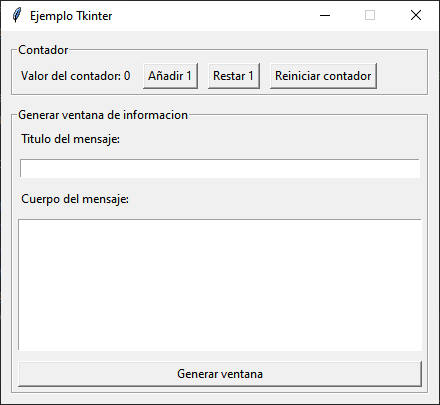
\includegraphics[width=0.6\linewidth]{fig/Ejemplo Tkinter/ventana principal.png}
    \caption{Ventana de la aplicación de ejemplo}
    \label{fig:principalWindowExample}
\end{figure}

Teniendo la interfaz de la aplicación de ejemplo, ya se puede comprobar que el funcionamiento sea el esperado, es decir, que todos los botones invoquen correctamente las funciones asociadas a ellos.

Primero se prueba que el botón del contador que añade unidades a este, invoque correctamente a la función que tiene asociada, es decir, la función \texttt{addOneToCounter} (Listado~\ref{src:addOneToCounterExample}) y que sume 1 al contador cada vez que este botón se pulse.

La función \texttt{addOneToCounter} primero suma 1 al valor del contador en el momento de su invocación. Tras esto, actualiza el texto de la etiqueta que muestra el valor del contador y, por último, actualiza toda la interfaz para que los cambios realizados sean visibles para el usuario.

\begin{lstlisting}[language=Python,
                   style=python,
                   frame=none,
                   numbers=none,
                   basicstyle=\ttfamily\normalsize,
                   caption={Función \texttt{addOneToCounter} del ejemplo de Tkinter},
                   label=src:addOneToCounterExample,
                   inputencoding=utf8]                   
def addOneToCounter(self):
    self.counter+=1
    self.labelForCounter.config(text=f"Valor del contador: {self.counter}")
    self.root.update_idletasks()
\end{lstlisting}

Para la prueba se ha pulsado 5 veces el botón "Añadir 1" en la interfaz, cuyo resultado puede apreciarse en la Figura~\ref{fig:counterFiveExample}.

\begin{figure}[H]
    \centering
    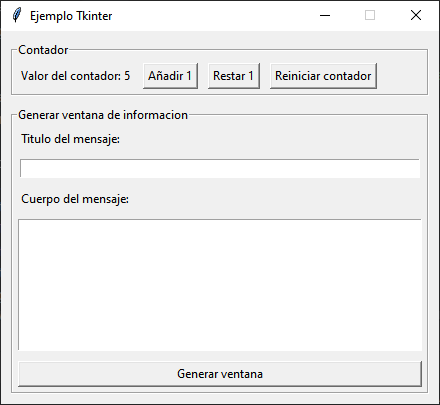
\includegraphics[width=0.6\linewidth]{fig/Ejemplo Tkinter/contador 5.png}
    \caption{Prueba del botón "Añadir 1"}
    \label{fig:counterFiveExample}
\end{figure}

Después, se ha comprobado que el botón "Resta 1" llame correctamente a la función que tiene asociada, en este caso \texttt{diffOneToCounter} (Listado~\ref{src:diffOneToCounterExample}). Esta función funciona de forma similar a la anterior, pero en lugar de sumar 1 al valor del contador que posea en el momento en el que se pulsa el botón, esta función resta 1 al valor actual del contador, cambia el texto que aparece en la etiqueta y actualiza toda la interfaz para que se reflejen los cambios.

\begin{lstlisting}[language=Python,
                   style=python,
                   frame=none,
                   numbers=none,
                   basicstyle=\ttfamily\normalsize,
                   caption={Función \texttt{diffOneToCounter} del ejemplo de Tkinter},
                   label=src:diffOneToCounterExample,
                   inputencoding=utf8]                   
def diffOneToCounter(self):
    self.counter-=1
    self.labelForCounter.config(text=f"Valor del contador: {self.counter}")
    self.root.update_idletasks()
\end{lstlisting}

Para comprobar que funciona, se ha pulsado una vez el botón que resta 1 al contador cuando el contador tenía un valor de 5, como se muestra en la Figura~\ref{fig:counterFiveExample}. Después de haber presionado el botón, el valor del contador baja a 4, como se puede ver en la Figura~\ref{fig:counterFourExample}

\begin{figure}[H]
    \centering
    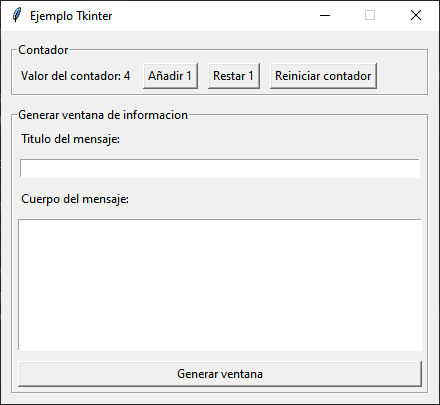
\includegraphics[width=0.6\linewidth]{fig/Ejemplo Tkinter/contador 4.png}
    \caption{Prueba del botón "Restar 1"}
    \label{fig:counterFourExample}
\end{figure}

Tras esto, se ha comprobado el funcionamiento del botón que reinicia el contador y lo pone a 0. Este botón lanza la función \texttt{resetCounter} (Listado~\ref{src:resetCounterExample}), que establece el valor de la variable que almacena el valor del contador a 0, actualiza la etiqueta que muestra el valor del contador y actualiza la ventana para que se reflejen todos los cambios realizados.

\begin{lstlisting}[language=Python,
                   style=python,
                   frame=none,
                   numbers=none,
                   basicstyle=\ttfamily\normalsize,
                   caption={Función \texttt{resetCounter} del ejemplo de Tkinter},
                   label=src:resetCounterExample,
                   inputencoding=utf8]                   
def resetCounter(self):
    self.counter = 0
    self.labelForCounter.config(text=f"Valor del contador: {self.counter}")
    self.root.update_idletasks()
\end{lstlisting}

Una vez pulsado el botón "Reiniciar contador" el contador pasa de tener un valor de 4 a tener un valor de 0, quedando la ventana como en la Figura~\ref{fig:principalWindowExample}, donde se veía el programa recién iniciado.

Por último, se prueba el funcionamiento del generador de ventanas de mensaje, escribiendo para ello un título para dicha ventana y un texto que aparecerá como mensaje en la ventana. Tanto el título como el cuerpo del mensaje se pueden ver en la Figura~\ref{fig:messagePrincipalWindowExample}.

\begin{figure}[H]
    \centering
    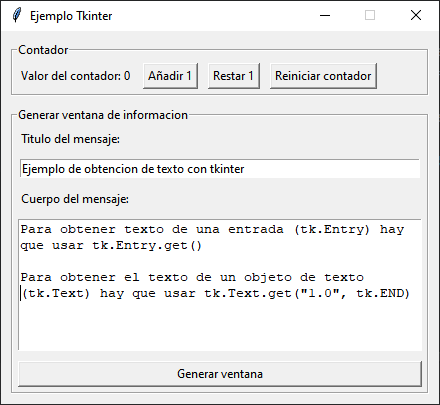
\includegraphics[width=0.6\linewidth]{fig/Ejemplo Tkinter/ventana principal con mensaje escrito.png}
    \caption{Ventana principal con los campos de título y cuerpo del mensaje rellenos}
    \label{fig:messagePrincipalWindowExample}
\end{figure}

Una vez obtenidos el título y el cuerpo del mensaje escritos, se presiona el botón "Generar ventana". Esto ejecuta la función \texttt{generateMsgInfoWinodw} (Listado~\ref{src:generateMsgInfoWindowExample}), encargada de generar la ventana de mensaje con los datos introducidos en la interfaz.

\begin{lstlisting}[language=Python,
                   style=python,
                   frame=none,
                   numbers=none,
                   basicstyle=\ttfamily\normalsize,
                   caption={Función \texttt{generateMsgInfoWinodw} del ejemplo de Tkinter},
                   label=src:generateMsgInfoWindowExample,
                   inputencoding=utf8]                   
def generateMsgInfoWinodw(self):
    title = self.titleEntry.get()
    message = self.messageText.get("1.0", tk.END)
    messagebox.showinfo(title=title, message=message)
\end{lstlisting}

La ventana generada, con los datos que aparecen en la Figura~\ref{fig:messagePrincipalWindowExample}, se muestra en la Figura \ref{fig:messageWindowExample}. 

\begin{figure}[H]
    \centering
    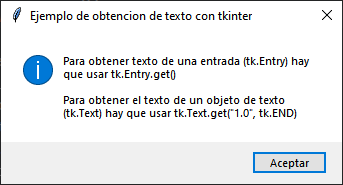
\includegraphics[width=0.5\linewidth]{fig/Ejemplo Tkinter/ventana generada con mensaje.png}
    \caption{Ventana de mensaje generada}
    \label{fig:messageWindowExample}
\end{figure}

\subsubsection{Interfaz del programa principal}

La interfaz del programa objeto de este \acrshort{TFG} se encuentra definida en el módulo \texttt{UI.py}. Al igual que en el ejemplo anterior, esta interfaz cuenta con una clase denominada \texttt{UI}, encargada de generar y gestionar todos los aspectos relacionados con la presentación y el funcionamiento de la aplicación. El constructor (Listado~\ref{src:uiClassConstructor}) de dicha clase no solo incluye lo necesario para construir la interfaz, como el título de la ventana, el protocolo para su cierre y el ícono que se muestra en la esquina superior izquierda, sino que también establece las referencias y crea instancias de los distintos módulos que componen la aplicación. De este modo, la interfaz puede acceder a cada uno de ellos, facilitando la interacción y la coordinación entre la lógica de la interfaz y el resto de los módulos.

\begin{lstlisting}[language=Python,
                   style=python,
                   frame=none,
                   numbers=none,
                   basicstyle=\ttfamily\normalsize,
                   caption={Constructor de la clase \texttt{UI}},
                   label=src:uiClassConstructor,
                   inputencoding=utf8]                   
def __init__(self):
    self.root = tk.Tk()  # Inicializacion de la ventana
    self.root.withdraw()
    self.root.title("TFG - Gestor de base de datos")  # Establecimiento del nombre de la ventana
    icon = tk.PhotoImage(file=os.path.join(getattr(sys, '_MEIPASS', os.path.dirname(os.path.abspath(__file__))),"icon.png"))
    self.root.iconphoto(False,icon)
    self.root.columnconfigure(0, weight=1)  # Activacion del autoajuste de la columna 0
    self.root.resizable(False, False)  # Restriccion del redimensionamiento de la ventana principal
    self.root.protocol("WM_DELETE_WINDOW",
                       self.onCloseEvent)  # Registro de la función a ejecutar al cerrar la aplicacion
    self.supplyLoger = SupplyLoger  # Inicializacion del objeto SupplyLoger
    self.demandLoger = DemandLoger  # Inicializacion del objeto DemandLoger
    self.resultsLoger = ResultsLoger  # Inicializacion del objeto ResultsLoger
    self.ymlParser = Parser()  # Inicializacion del módulo yamlParser
    self.ymlWriter = Writer()  # Inicializacion del módulo yamlWriter
    self.sqlSupply = SqlSupply()  # Inicializacion del objeto SqlSupply del módulo SQLHandler
    self.sqlDemand = SqlDemand()  # Inicializacion del objeto SqlDemand del módulo SQLHandler
    self.sqlResults = SqlResults()  # Inicializacion del objeto SqlResults del módulo SQLHandler
    self.config = Config()  # Inicializacion del módulo configManager
    self.csvReader = csvReader()  # Inicializacion del objeto csvReader del módulo csvHandler
    self.csvWriter = csvWriter  # Inicializacion del objeto csvWriter del módulo csvHandler
    self.init_ui()  # Inicializacion de la interfaz
    self.root.deiconify()
\end{lstlisting}

La distribución de la interfaz del programa se muestra en la Figura~\ref{fig:mainWindow}. En ella se pueden apreciar, por ejemplo, los botones destinados a la importación de los datos de los archivos en cada una de las bases de datos, los botones para la exportación de datos a un archivo desde las bases de datos, así como los que permiten eliminar los datos asociados a un archivo específico. También se encuentra un apartado dedicado a la interacción con las bases de datos mediante sentencias \acrshort{SQL}, en el que se pueden ejecutar sentencias previamente almacenadas, cargar un archivo con extensión \texttt{.sql} que contenga la sentencia \acrshort{SQL} o, alternativamente, escribir la sentencia directamente en la zona de texto destinada para ello. 

\begin{figure}[H]
    \centering
    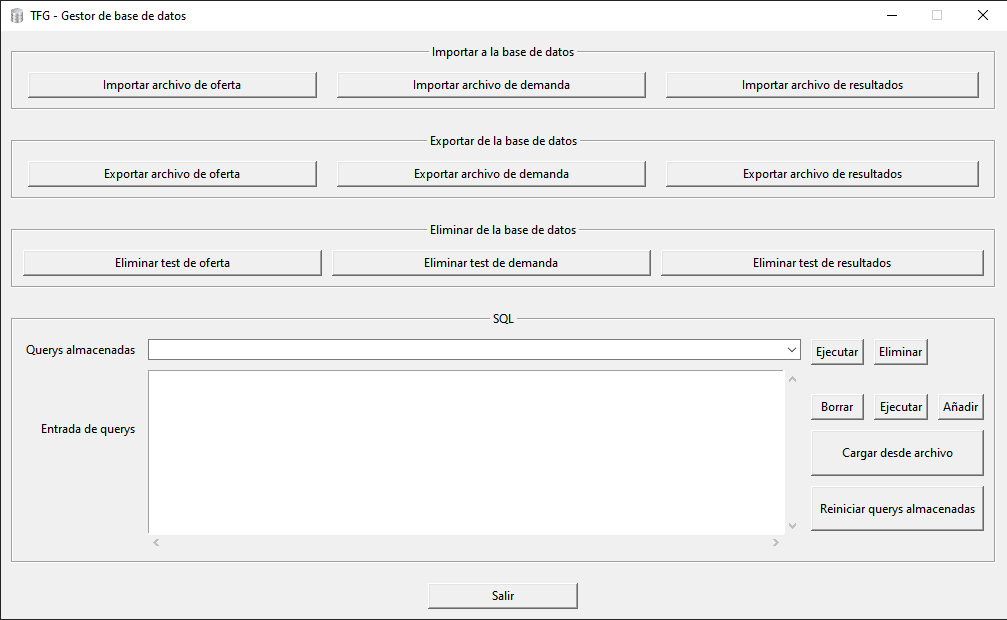
\includegraphics[width=1\linewidth]{fig/Interfaz de la aplicación/ventana principal.png}
    \caption{Ventana principal de la aplicación}
    \label{fig:mainWindow}
\end{figure}

Las sentencias que son cargadas desde un archivo o escritas directamente en la interfaz se someten a un proceso de validación antes de ser ejecutadas. Esto evita que se ejecuten sentencias en la base de datos que presenten errores, como por ejemplo, errores sintácticos. Si se detecta algún error durante la validación, se notificará al usuario mediante una ventana emergente el error presente en la sentencia. En las Figuras \ref{fig:queryWithColumnError} y \ref{fig:messageQueryWithColumnError} se puede apreciar una sentencia con un error; en este caso, la columna "campoInexistente" no existe dentro de la base de datos de los archivos de la oferta, y su correspondiente mensaje indicando que la columna requerida por el usuario no existe en la base de datos.

\begin{figure}[H]
    \centering
    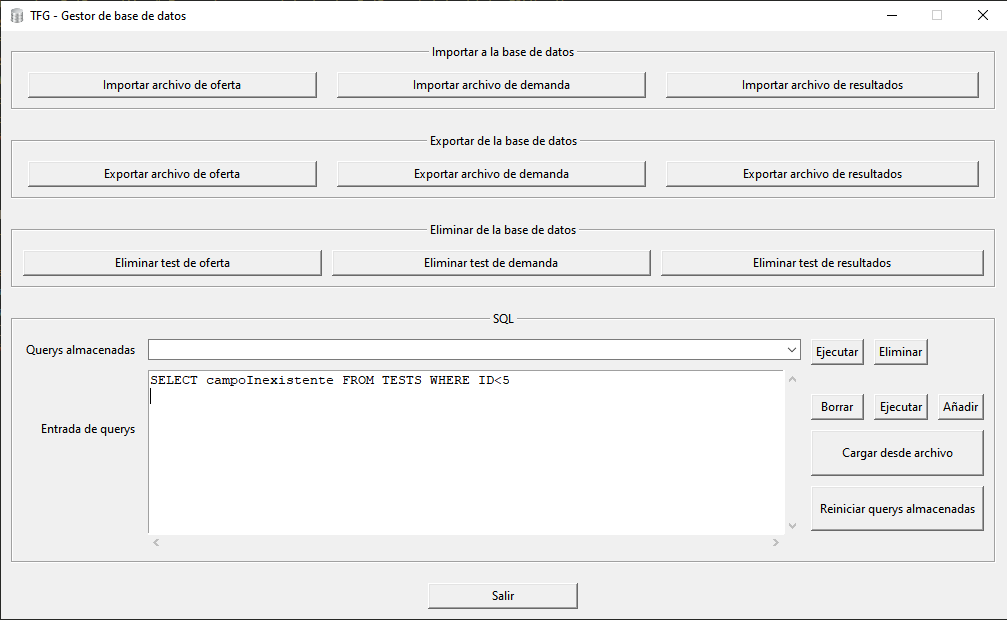
\includegraphics[width=1\linewidth]{"fig/Interfaz de la aplicación/consulta con error.png"}
    \caption{sentencia con error de columna faltante}
    \label{fig:queryWithColumnError}
\end{figure}


\begin{figure}[H]
    \centering
    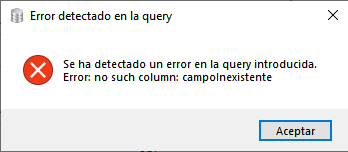
\includegraphics[width=0.5\linewidth]{fig/Interfaz de la aplicación/resultados de la consulta con error.png}
    \caption{Mensaje de error al ejecutar la sentencia con error de la Figura~\ref{fig:queryWithColumnError}}
    \label{fig:messageQueryWithColumnError}
\end{figure}


